\PassOptionsToPackage{unicode=true}{hyperref} % options for packages loaded elsewhere
\PassOptionsToPackage{hyphens}{url}
%
\documentclass[]{article}
\usepackage{lmodern}
\usepackage{amssymb,amsmath}
\usepackage{ifxetex,ifluatex}
\usepackage{fixltx2e} % provides \textsubscript
\ifnum 0\ifxetex 1\fi\ifluatex 1\fi=0 % if pdftex
  \usepackage[T1]{fontenc}
  \usepackage[utf8]{inputenc}
  \usepackage{textcomp} % provides euro and other symbols
\else % if luatex or xelatex
  \usepackage{unicode-math}
  \defaultfontfeatures{Ligatures=TeX,Scale=MatchLowercase}
\fi
% use upquote if available, for straight quotes in verbatim environments
\IfFileExists{upquote.sty}{\usepackage{upquote}}{}
% use microtype if available
\IfFileExists{microtype.sty}{%
\usepackage[]{microtype}
\UseMicrotypeSet[protrusion]{basicmath} % disable protrusion for tt fonts
}{}
\IfFileExists{parskip.sty}{%
\usepackage{parskip}
}{% else
\setlength{\parindent}{0pt}
\setlength{\parskip}{6pt plus 2pt minus 1pt}
}
\usepackage{hyperref}
\hypersetup{
            pdftitle={Sex and Power: Sexual dimorphism in trait variability and its eco-evolutionary and statistical implications},
            pdfauthor={Susanne Zajitschek, Felix Zajitschek, Russell Bonduriansky, Robert Brooks, Will Cornwell, Daniel Falster, Malgorzata Lagisz, Jeremy Mason, Alistair Senior, Daniel Noble, \& Shinichi Nakagawa},
            pdfborder={0 0 0},
            breaklinks=true}
\urlstyle{same}  % don't use monospace font for urls
\usepackage[margin=1in]{geometry}
\usepackage{color}
\usepackage{fancyvrb}
\newcommand{\VerbBar}{|}
\newcommand{\VERB}{\Verb[commandchars=\\\{\}]}
\DefineVerbatimEnvironment{Highlighting}{Verbatim}{commandchars=\\\{\}}
% Add ',fontsize=\small' for more characters per line
\usepackage{framed}
\definecolor{shadecolor}{RGB}{248,248,248}
\newenvironment{Shaded}{\begin{snugshade}}{\end{snugshade}}
\newcommand{\AlertTok}[1]{\textcolor[rgb]{0.94,0.16,0.16}{#1}}
\newcommand{\AnnotationTok}[1]{\textcolor[rgb]{0.56,0.35,0.01}{\textbf{\textit{#1}}}}
\newcommand{\AttributeTok}[1]{\textcolor[rgb]{0.77,0.63,0.00}{#1}}
\newcommand{\BaseNTok}[1]{\textcolor[rgb]{0.00,0.00,0.81}{#1}}
\newcommand{\BuiltInTok}[1]{#1}
\newcommand{\CharTok}[1]{\textcolor[rgb]{0.31,0.60,0.02}{#1}}
\newcommand{\CommentTok}[1]{\textcolor[rgb]{0.56,0.35,0.01}{\textit{#1}}}
\newcommand{\CommentVarTok}[1]{\textcolor[rgb]{0.56,0.35,0.01}{\textbf{\textit{#1}}}}
\newcommand{\ConstantTok}[1]{\textcolor[rgb]{0.00,0.00,0.00}{#1}}
\newcommand{\ControlFlowTok}[1]{\textcolor[rgb]{0.13,0.29,0.53}{\textbf{#1}}}
\newcommand{\DataTypeTok}[1]{\textcolor[rgb]{0.13,0.29,0.53}{#1}}
\newcommand{\DecValTok}[1]{\textcolor[rgb]{0.00,0.00,0.81}{#1}}
\newcommand{\DocumentationTok}[1]{\textcolor[rgb]{0.56,0.35,0.01}{\textbf{\textit{#1}}}}
\newcommand{\ErrorTok}[1]{\textcolor[rgb]{0.64,0.00,0.00}{\textbf{#1}}}
\newcommand{\ExtensionTok}[1]{#1}
\newcommand{\FloatTok}[1]{\textcolor[rgb]{0.00,0.00,0.81}{#1}}
\newcommand{\FunctionTok}[1]{\textcolor[rgb]{0.00,0.00,0.00}{#1}}
\newcommand{\ImportTok}[1]{#1}
\newcommand{\InformationTok}[1]{\textcolor[rgb]{0.56,0.35,0.01}{\textbf{\textit{#1}}}}
\newcommand{\KeywordTok}[1]{\textcolor[rgb]{0.13,0.29,0.53}{\textbf{#1}}}
\newcommand{\NormalTok}[1]{#1}
\newcommand{\OperatorTok}[1]{\textcolor[rgb]{0.81,0.36,0.00}{\textbf{#1}}}
\newcommand{\OtherTok}[1]{\textcolor[rgb]{0.56,0.35,0.01}{#1}}
\newcommand{\PreprocessorTok}[1]{\textcolor[rgb]{0.56,0.35,0.01}{\textit{#1}}}
\newcommand{\RegionMarkerTok}[1]{#1}
\newcommand{\SpecialCharTok}[1]{\textcolor[rgb]{0.00,0.00,0.00}{#1}}
\newcommand{\SpecialStringTok}[1]{\textcolor[rgb]{0.31,0.60,0.02}{#1}}
\newcommand{\StringTok}[1]{\textcolor[rgb]{0.31,0.60,0.02}{#1}}
\newcommand{\VariableTok}[1]{\textcolor[rgb]{0.00,0.00,0.00}{#1}}
\newcommand{\VerbatimStringTok}[1]{\textcolor[rgb]{0.31,0.60,0.02}{#1}}
\newcommand{\WarningTok}[1]{\textcolor[rgb]{0.56,0.35,0.01}{\textbf{\textit{#1}}}}
\usepackage{graphicx,grffile}
\makeatletter
\def\maxwidth{\ifdim\Gin@nat@width>\linewidth\linewidth\else\Gin@nat@width\fi}
\def\maxheight{\ifdim\Gin@nat@height>\textheight\textheight\else\Gin@nat@height\fi}
\makeatother
% Scale images if necessary, so that they will not overflow the page
% margins by default, and it is still possible to overwrite the defaults
% using explicit options in \includegraphics[width, height, ...]{}
\setkeys{Gin}{width=\maxwidth,height=\maxheight,keepaspectratio}
\setlength{\emergencystretch}{3em}  % prevent overfull lines
\providecommand{\tightlist}{%
  \setlength{\itemsep}{0pt}\setlength{\parskip}{0pt}}
\setcounter{secnumdepth}{0}
% Redefines (sub)paragraphs to behave more like sections
\ifx\paragraph\undefined\else
\let\oldparagraph\paragraph
\renewcommand{\paragraph}[1]{\oldparagraph{#1}\mbox{}}
\fi
\ifx\subparagraph\undefined\else
\let\oldsubparagraph\subparagraph
\renewcommand{\subparagraph}[1]{\oldsubparagraph{#1}\mbox{}}
\fi

% set default figure placement to htbp
\makeatletter
\def\fps@figure{htbp}
\makeatother

\usepackage{etoolbox}
\makeatletter
\providecommand{\subtitle}[1]{% add subtitle to \maketitle
  \apptocmd{\@title}{\par {\large #1 \par}}{}{}
}
\makeatother
\usepackage{booktabs}
\usepackage{longtable}
\usepackage{array}
\usepackage{multirow}
\usepackage{wrapfig}
\usepackage{float}
\usepackage{colortbl}
\usepackage{pdflscape}
\usepackage{tabu}
\usepackage{threeparttable}
\usepackage{threeparttablex}
\usepackage[normalem]{ulem}
\usepackage{makecell}
\usepackage{xcolor}

\title{Sex and Power: Sexual dimorphism in trait variability and its
eco-evolutionary and statistical implications}
\providecommand{\subtitle}[1]{}
\subtitle{Electronic Supplementary Material}
\author{Susanne Zajitschek, Felix Zajitschek, Russell Bonduriansky, Robert
Brooks, Will Cornwell, Daniel Falster, Malgorzata Lagisz, Jeremy Mason,
Alistair Senior, Daniel Noble, \& Shinichi Nakagawa}
\date{2020-05-19}

\begin{document}
\maketitle

{
\setcounter{tocdepth}{4}
\tableofcontents
}
\hypertarget{general-introduction}{%
\section{General Introduction}\label{general-introduction}}

This supplementary material follows the general structure described in
our methods and is outlined here in Figure @ref(fig:FigG1). Generally
speaking, the first few sections describe the processes by which the
data were cleaned and re-organised for analysis. This iss followed by
how the first order and second order meta-analsyes were conducted.
Supplemental tables and figures that are referenecd within the main
manuscript can be found at the end of the document. Various parts of the
workflow can be conviently referenecd using the side table of contents
panel. We will refer back to this figure as we describe the various
aspects of the code and data processing in relevant places.

\begin{Shaded}
\begin{Highlighting}[]
\KeywordTok{include_graphics}\NormalTok{(}\KeywordTok{here}\NormalTok{(}\StringTok{"images"}\NormalTok{, }\StringTok{"workflow.png"}\NormalTok{))}
\end{Highlighting}
\end{Shaded}

\begin{figure}
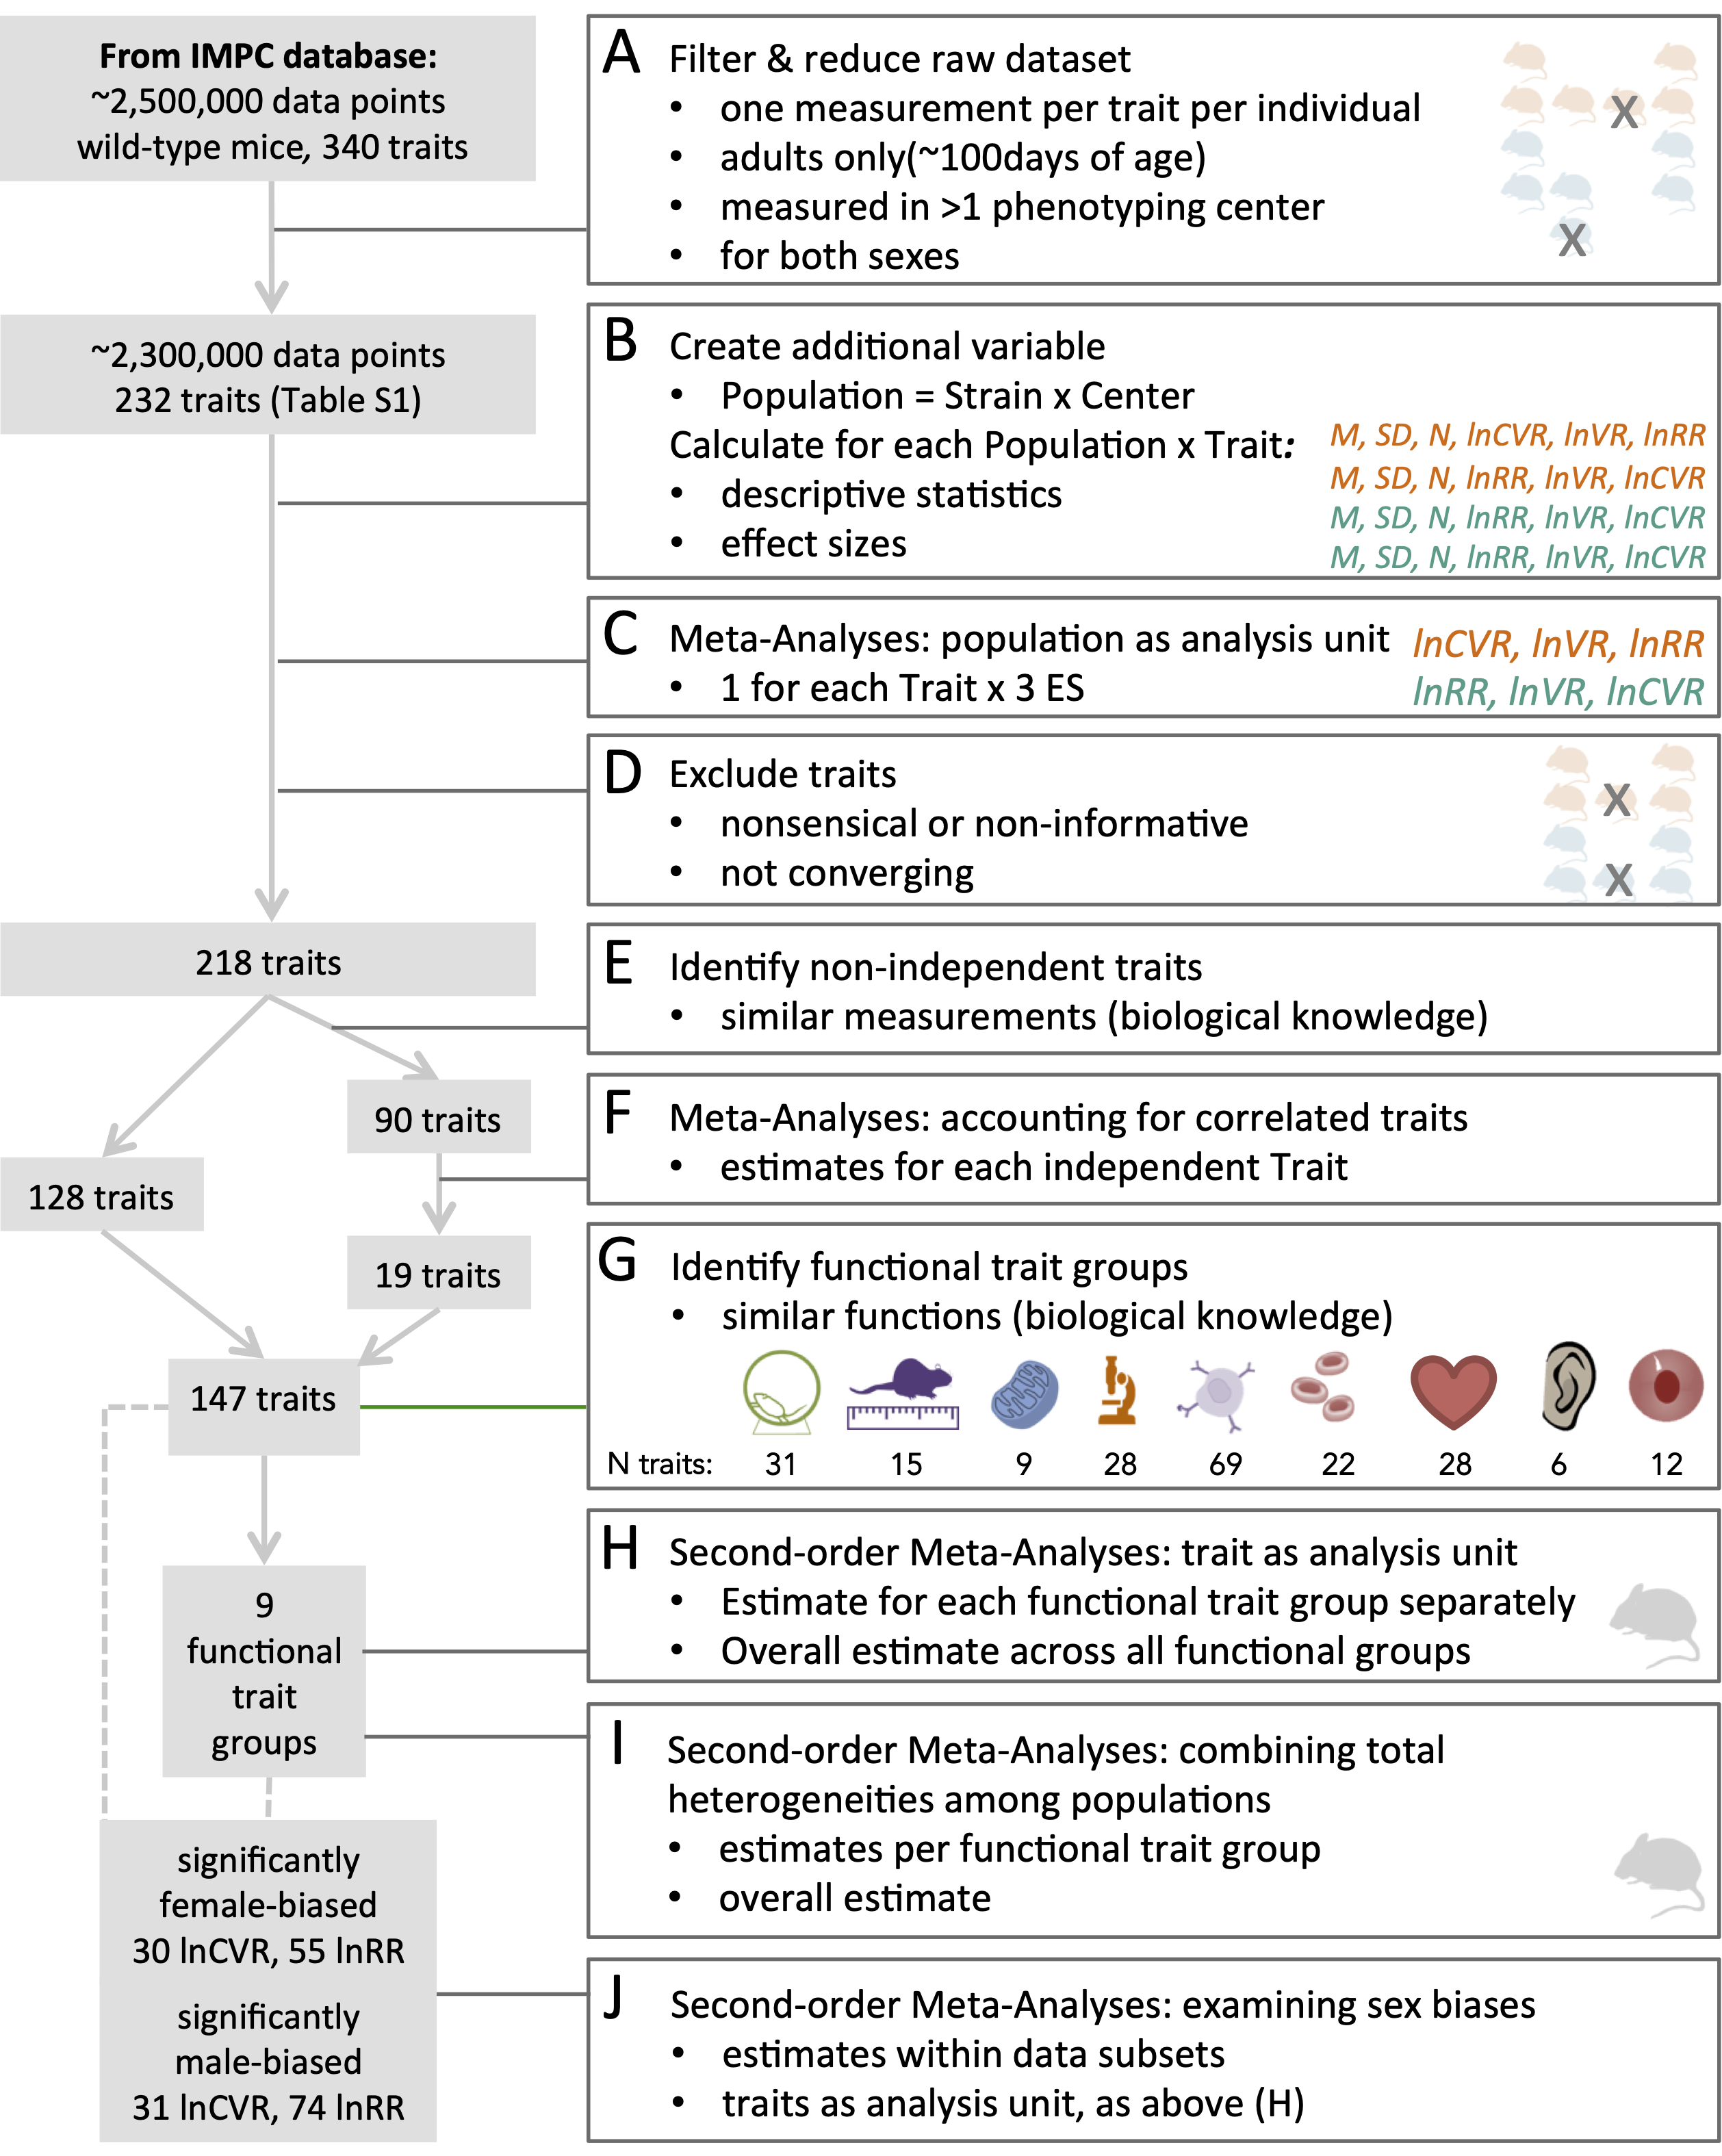
\includegraphics[width=34.94in]{/Users/danielnoble/Dropbox/1_Research/1_Manuscripts/In_Preparation/mice_sex_diff/images/workflow} \caption{Workflow of data process and meta-analysis}\label{fig:FigG1}
\end{figure}

\hypertarget{set-up}{%
\section{Set-up}\label{set-up}}

\hypertarget{packages}{%
\subsection{Packages}\label{packages}}

\begin{Shaded}
\begin{Highlighting}[]
\KeywordTok{library}\NormalTok{(pacman)}
\NormalTok{pacman}\OperatorTok{::}\KeywordTok{p_load}\NormalTok{(readr, dplyr, metafor, devtools, purrr, tidyverse, tidyr, tibble, }
\NormalTok{    kableExtra, robumeta, ggpubr, ggplot2, png, grid, here, pander)}
\end{Highlighting}
\end{Shaded}

\hypertarget{functions}{%
\subsection{Functions}\label{functions}}

Functions needed for preparing the data for meta analyses

\hypertarget{loading-and-cleaning-data}{%
\subsubsection{Loading and cleaning
data}\label{loading-and-cleaning-data}}

These functions will load the raw and and do some cleaning to make it
ready for further processing and analysis.

\begin{Shaded}
\begin{Highlighting}[]
\CommentTok{# loads the raw data, setting some default types for various columns}

\NormalTok{load_raw <-}\StringTok{ }\ControlFlowTok{function}\NormalTok{(filename) \{}
    \KeywordTok{read_csv}\NormalTok{(filename, }\DataTypeTok{col_types =} \KeywordTok{cols}\NormalTok{(}\DataTypeTok{.default =} \KeywordTok{col_character}\NormalTok{(), }\DataTypeTok{project_id =} \KeywordTok{col_character}\NormalTok{(), }
        \DataTypeTok{id =} \KeywordTok{col_character}\NormalTok{(), }\DataTypeTok{parameter_id =} \KeywordTok{col_character}\NormalTok{(), }\DataTypeTok{age_in_days =} \KeywordTok{col_integer}\NormalTok{(), }
        \DataTypeTok{date_of_experiment =} \KeywordTok{col_datetime}\NormalTok{(}\DataTypeTok{format =} \StringTok{""}\NormalTok{), }\DataTypeTok{weight =} \KeywordTok{col_double}\NormalTok{(), }\DataTypeTok{phenotyping_center_id =} \KeywordTok{col_character}\NormalTok{(), }
        \DataTypeTok{production_center_id =} \KeywordTok{col_character}\NormalTok{(), }\DataTypeTok{weight_date =} \KeywordTok{col_datetime}\NormalTok{(}\DataTypeTok{format =} \StringTok{""}\NormalTok{), }
        \DataTypeTok{date_of_birth =} \KeywordTok{col_datetime}\NormalTok{(}\DataTypeTok{format =} \StringTok{""}\NormalTok{), }\DataTypeTok{procedure_id =} \KeywordTok{col_character}\NormalTok{(), }
        \DataTypeTok{pipeline_id =} \KeywordTok{col_character}\NormalTok{(), }\DataTypeTok{biological_sample_id =} \KeywordTok{col_character}\NormalTok{(), }\DataTypeTok{biological_model_id =} \KeywordTok{col_character}\NormalTok{(), }
        \DataTypeTok{weight_days_old =} \KeywordTok{col_integer}\NormalTok{(), }\DataTypeTok{datasource_id =} \KeywordTok{col_character}\NormalTok{(), }\DataTypeTok{experiment_id =} \KeywordTok{col_character}\NormalTok{(), }
        \DataTypeTok{data_point =} \KeywordTok{col_double}\NormalTok{(), }\DataTypeTok{age_in_weeks =} \KeywordTok{col_integer}\NormalTok{(), }\StringTok{`}\DataTypeTok{_version_}\StringTok{`}\NormalTok{ =}\StringTok{ }\KeywordTok{col_character}\NormalTok{()))}
\NormalTok{\}}

\CommentTok{# Apply some standard cleaning to the data}
\NormalTok{clean_raw_data <-}\StringTok{ }\ControlFlowTok{function}\NormalTok{(mydata) \{}
    
\NormalTok{    group <-}\StringTok{ }\KeywordTok{read_csv}\NormalTok{(}\KeywordTok{here}\NormalTok{(}\StringTok{"data"}\NormalTok{, }\StringTok{"ParameterGrouping.csv"}\NormalTok{))}
    
\NormalTok{    tmp <-}\StringTok{ }\NormalTok{mydata }\OperatorTok\StringTok{ }
\StringTok{    }\CommentTok{# Filter to IMPC source (recommend by Jeremey in email to Susi on 20 Aug 2018)}
\StringTok{    }\KeywordTok{filter}\NormalTok{(datasource_name }\OperatorTok{==}\StringTok{ "IMPC"}\NormalTok{) }\OperatorTok\StringTok{ }
\StringTok{    }\CommentTok{# standardise trait names}
\StringTok{    }\KeywordTok{mutate}\NormalTok{(}\DataTypeTok{parameter_name =} \KeywordTok{tolower}\NormalTok{(parameter_name)) }\OperatorTok\StringTok{ }
\StringTok{    }\CommentTok{# remove extreme ages}
\StringTok{    }\KeywordTok{filter}\NormalTok{(age_in_days }\OperatorTok{>}\StringTok{ }\DecValTok{0} \OperatorTok{&}\StringTok{ }\NormalTok{age_in_days }\OperatorTok{<}\StringTok{ }\DecValTok{500}\NormalTok{) }\OperatorTok\StringTok{ }
\StringTok{    }\CommentTok{# remove NAs}
\StringTok{    }\KeywordTok{filter}\NormalTok{(}\OperatorTok{!}\KeywordTok{is.na}\NormalTok{(data_point)) }\OperatorTok\StringTok{ }
\StringTok{    }\CommentTok{# subset to reasonable set of variables, date_of_experiment used as an indicator}
\StringTok{    }\CommentTok{# of batch-level effects}
\StringTok{    }\KeywordTok{select}\NormalTok{(production_center, strain_name, strain_accession_id, biological_sample_id, }
\NormalTok{        pipeline_stable_id, procedure_group, procedure_name, sex, date_of_experiment, }
\NormalTok{        age_in_days, weight, parameter_name, data_point) }\OperatorTok\StringTok{ }
\StringTok{    }\CommentTok{# sort}
\StringTok{    }\KeywordTok{arrange}\NormalTok{(production_center, biological_sample_id, age_in_days)}
    
    \CommentTok{# filter to groups with > 1 centre}
    \KeywordTok{merge}\NormalTok{(tmp, tmp }\OperatorTok\StringTok{ }\KeywordTok{group_by}\NormalTok{(parameter_name) }\OperatorTok\StringTok{ }\KeywordTok{summarise}\NormalTok{(}\DataTypeTok{center_per_trait =} \KeywordTok{length}\NormalTok{(}\KeywordTok{unique}\NormalTok{(production_center, }
        \DataTypeTok{na.rm =} \OtherTok{TRUE}\NormalTok{)))) }\OperatorTok\StringTok{ }\KeywordTok{filter}\NormalTok{(center_per_trait }\OperatorTok{>=}\StringTok{ }\DecValTok{2}\NormalTok{) }\OperatorTok\StringTok{ }
\StringTok{    }\CommentTok{# Define population variable}
\StringTok{    }\KeywordTok{mutate}\NormalTok{(}\DataTypeTok{population =} \KeywordTok{sprintf}\NormalTok{(}\StringTok{"%s-%s"}\NormalTok{, production_center, strain_name)) }\OperatorTok\StringTok{ }
\StringTok{    }\CommentTok{# add grouping variable: these were decided based on functional groups and}
\StringTok{    }\CommentTok{# procedures}
\StringTok{    }\KeywordTok{mutate}\NormalTok{(}\DataTypeTok{parameter_group =}\NormalTok{ group}\OperatorTok{$}\NormalTok{parameter[}\KeywordTok{match}\NormalTok{(parameter_name, group}\OperatorTok{$}\NormalTok{parameter_name)]) }\OperatorTok\StringTok{ }
\StringTok{        }
\StringTok{    }\CommentTok{# Assign unique IDs (per trait) each unique parameter_name (=trait,use trait}
\StringTok{    }\CommentTok{# variable) gets a unique number ('id')}
\StringTok{    }
\StringTok{    }\CommentTok{# We add a new variable, where redundant traits are combined [note however, at}
\StringTok{    }\CommentTok{# this stage the dataset still contains nonsensical traits, i.e. traits that may}
\StringTok{    }\CommentTok{# not contain any information on variance]}
\StringTok{    }\KeywordTok{mutate}\NormalTok{(}\DataTypeTok{id =} \KeywordTok{match}\NormalTok{(parameter_name, }\KeywordTok{unique}\NormalTok{(parameter_name))) }\OperatorTok\StringTok{ }\KeywordTok{as_tibble}\NormalTok{()}
\NormalTok{\}}
\end{Highlighting}
\end{Shaded}

\hypertarget{sub-setting-data}{%
\subsubsection{Sub-setting data}\label{sub-setting-data}}

Create a function for sub-setting the data to choose only one data point
per individual per trait:
``data\_subset\_parameterid\_individual\_by\_age''

\begin{Shaded}
\begin{Highlighting}[]
\NormalTok{data_subset_parameterid_individual_by_age <-}\StringTok{ }\ControlFlowTok{function}\NormalTok{(mydata, parameter, }\DataTypeTok{age_min =} \DecValTok{0}\NormalTok{, }
    \DataTypeTok{age_center =} \DecValTok{100}\NormalTok{) \{}
\NormalTok{    tmp <-}\StringTok{ }\NormalTok{mydata }\OperatorTok\StringTok{ }\KeywordTok{filter}\NormalTok{(age_in_days }\OperatorTok{>=}\StringTok{ }\NormalTok{age_min, id }\OperatorTok{==}\StringTok{ }\NormalTok{parameter) }\OperatorTok\StringTok{ }\CommentTok{# Take results for single individual closest to age_center}
\StringTok{    }\KeywordTok{mutate}\NormalTok{(}\DataTypeTok{age_diff =} \KeywordTok{abs}\NormalTok{(age_center }\OperatorTok{-}\StringTok{ }\NormalTok{age_in_days)) }\OperatorTok\StringTok{ }\KeywordTok{group_by}\NormalTok{(biological_sample_id) }\OperatorTok\StringTok{ }
\StringTok{        }\KeywordTok{filter}\NormalTok{(age_diff }\OperatorTok{==}\StringTok{ }\KeywordTok{min}\NormalTok{(age_diff)) }\OperatorTok\StringTok{ }\KeywordTok{select}\NormalTok{(}\OperatorTok{-}\NormalTok{age_diff)}
    
    \CommentTok{# Still some individuals with multiple records (because same individual appears}
    \CommentTok{# under different procedures, so filter to one record)}
\NormalTok{    j <-}\StringTok{ }\KeywordTok{match}\NormalTok{(}\KeywordTok{unique}\NormalTok{(tmp}\OperatorTok{$}\NormalTok{biological_sample_id), tmp}\OperatorTok{$}\NormalTok{biological_sample_id)}
\NormalTok{    tmp[j, ]}
\NormalTok{\}}
\end{Highlighting}
\end{Shaded}

\hypertarget{population-statistics}{%
\subsubsection{Population statistics}\label{population-statistics}}

Create a function called: ``calculate\_population\_stats'' This function
groups animals from the same strain and institution together. This is
done for each trait separately, and only for traits that have been
measured in both sexes. Any group containing fewer than 6 individuals is
excluded.

\begin{Shaded}
\begin{Highlighting}[]
\CommentTok{# Function re-organises the data so that the male and female data are side-by-side as columns to make effect size calculations easier.}
\NormalTok{multi_spread <-}\StringTok{ }\ControlFlowTok{function}\NormalTok{(df, key, value) \{}
    \CommentTok{# quote key}
\NormalTok{      keyq <-}\StringTok{ }\NormalTok{rlang}\OperatorTok{::}\KeywordTok{enquo}\NormalTok{(key)}
    \CommentTok{# break value vector into quotes}
\NormalTok{    valueq <-}\StringTok{ }\NormalTok{rlang}\OperatorTok{::}\KeywordTok{enquo}\NormalTok{(value)}
\NormalTok{         s <-}\StringTok{ }\NormalTok{rlang}\OperatorTok{::}\KeywordTok{quos}\NormalTok{(}\OperatorTok{!!}\NormalTok{valueq)}
        
\NormalTok{         df                           }\OperatorTok\StringTok{ }
\StringTok{        }\KeywordTok{gather}\NormalTok{(variable, value, }\OperatorTok{!!!}\NormalTok{s) }\OperatorTok
\StringTok{        }\KeywordTok{unite}\NormalTok{(temp, }\OperatorTok{!!}\NormalTok{keyq, variable) }\OperatorTok
\StringTok{        }\KeywordTok{spread}\NormalTok{(temp, value)}
\NormalTok{\}}


\CommentTok{# Function will calculate population stats and exclude data that is irrelevant and not useful, it will also just convert the data straight away to wide format making it ready for effect size calculations}

\NormalTok{calculate_population_stats <-}\StringTok{ }\ControlFlowTok{function}\NormalTok{(mydata, }\DataTypeTok{min_individuals =} \DecValTok{5}\NormalTok{)\{}
\NormalTok{    mydata }\OperatorTok\StringTok{ }
\StringTok{    }\KeywordTok{group_by}\NormalTok{(population,}
\NormalTok{             production_center,  }
\NormalTok{             strain_name,  }
\NormalTok{             sex) }\OperatorTok
\StringTok{    }\KeywordTok{summarise}\NormalTok{(}\DataTypeTok{trait  =}\NormalTok{ parameter_name[}\DecValTok{1}\NormalTok{],}
              \DataTypeTok{x_bar  =} \KeywordTok{mean}\NormalTok{(data_point, }\DataTypeTok{na.rm =} \OtherTok{TRUE}\NormalTok{),}
              \DataTypeTok{x_sd   =}   \KeywordTok{sd}\NormalTok{(data_point, }\DataTypeTok{na.rm =} \OtherTok{TRUE}\NormalTok{),}
              \DataTypeTok{n_ind  =} \KeywordTok{n}\NormalTok{()) }\OperatorTok
\StringTok{    }\KeywordTok{ungroup}\NormalTok{() }\OperatorTok
\StringTok{    }\KeywordTok{filter}\NormalTok{(n_ind }\OperatorTok{>}\StringTok{ }\NormalTok{min_individuals) }\OperatorTok\StringTok{   }\CommentTok{# }\AlertTok{NOTE}\CommentTok{ here that you are excluding data with 5 exactly....}
\StringTok{    }\KeywordTok{group_by}\NormalTok{(population) }\OperatorTok
\StringTok{    }\KeywordTok{filter}\NormalTok{(}\KeywordTok{all}\NormalTok{(}\KeywordTok{c}\NormalTok{(}\StringTok{"male"}\NormalTok{, }\StringTok{"female"}\NormalTok{) }\OperatorTok\StringTok{ }\NormalTok{sex)) }\OperatorTok\StringTok{ }\CommentTok{# Removes any entries where only 1 sex is present}
\StringTok{    }\KeywordTok{multi_spread}\NormalTok{(sex, }\KeywordTok{c}\NormalTok{(x_bar, x_sd, n_ind))      }\CommentTok{# Spreads the data out into wide format, so sexes are beside each other which is more typical of meta-analytic data}
\NormalTok{\}}
\end{Highlighting}
\end{Shaded}

\hypertarget{calculate-effect-sizes-and-sample-variances}{%
\subsubsection{Calculate effect sizes and sample
variances}\label{calculate-effect-sizes-and-sample-variances}}

Function: ``create\_meta\_analysis\_effect\_sizes''

\begin{Shaded}
\begin{Highlighting}[]
\CommentTok{# This function takes the data and computes lnCVR, lnVR and ROM (lnRR) using male}
\CommentTok{# and female data to generate effect size statistics for meta-analyses}
\NormalTok{create_meta_analysis_effect_sizes <-}\StringTok{ }\ControlFlowTok{function}\NormalTok{(mydata, }\DataTypeTok{measure =} \KeywordTok{c}\NormalTok{(}\StringTok{"CVR"}\NormalTok{, }\StringTok{"VR"}\NormalTok{, }\StringTok{"ROM"}\NormalTok{)) \{}
    \ControlFlowTok{for}\NormalTok{ (i }\ControlFlowTok{in} \DecValTok{1}\OperatorTok{:}\KeywordTok{length}\NormalTok{(measure)) \{}
\NormalTok{        mydata <-}\StringTok{ }\NormalTok{metafor}\OperatorTok{::}\KeywordTok{escalc}\NormalTok{(}\DataTypeTok{m1i =}\NormalTok{ male_x_bar, }\DataTypeTok{m2i =}\NormalTok{ female_x_bar, }\DataTypeTok{sd1i =}\NormalTok{ male_x_sd, }
            \DataTypeTok{sd2i =}\NormalTok{ female_x_sd, }\DataTypeTok{n1i =}\NormalTok{ male_n_ind, }\DataTypeTok{n2i =}\NormalTok{ female_n_ind, }\DataTypeTok{data =}\NormalTok{ mydata, }
            \DataTypeTok{measure =}\NormalTok{ measure[i], }\DataTypeTok{var.names =} \KeywordTok{c}\NormalTok{(}\KeywordTok{paste0}\NormalTok{(}\StringTok{"effect_size_"}\NormalTok{, measure[i]), }
                \KeywordTok{paste0}\NormalTok{(}\StringTok{"sample_variance_"}\NormalTok{, measure[i])), }\DataTypeTok{append =} \OtherTok{TRUE}\NormalTok{)}
\NormalTok{    \}}
    \KeywordTok{return}\NormalTok{(mydata)}
\NormalTok{\}}
\end{Highlighting}
\end{Shaded}

\hypertarget{load-clean-data}{%
\subsection{Load \& clean data}\label{load-clean-data}}

We have already done this step and provide a cleaned up file which is
less computationally intensive to deal with. The file has been saved in
a folder called \texttt{export}. However, the \texttt{.csv} is provided
in case this is preferred and can be imported and processed using
following the steps below: {[}This code is currently excluded from
showing in this \texttt{.html} file, but can be viewed and enabled / run
in the down-loadable .rmd file. However, it requires the .gz file
containing the raw data in the ``export'' folder. Unfortunately, that
file can not be provided via Github, as it is too large (274MB).
However, it is freely accessible and uploaded to zenodo.org
(\url{https://zenodo.org/deposit/3759701})

\begin{Shaded}
\begin{Highlighting}[]
\CommentTok{# Load raw data - save cleaned dataset as RDS for reuse}
\NormalTok{data_raw <-}\StringTok{ }\KeywordTok{load_raw}\NormalTok{(}\KeywordTok{here}\NormalTok{(}\StringTok{"data"}\NormalTok{, }\StringTok{"dr7.0_all_control_data.csv.gz"}\NormalTok{))}
\KeywordTok{dir.create}\NormalTok{(}\StringTok{"export"}\NormalTok{, F, F)}

\NormalTok{data <-}\StringTok{ }\NormalTok{data_raw }\OperatorTok\StringTok{ }\KeywordTok{clean_raw_data}\NormalTok{()}
\KeywordTok{saveRDS}\NormalTok{(data, }\StringTok{"export/data_clean.rds"}\NormalTok{)}
\end{Highlighting}
\end{Shaded}

For analysis we load the RDS created above and other datasets

\begin{Shaded}
\begin{Highlighting}[]
\NormalTok{data <-}\StringTok{ }\KeywordTok{readRDS}\NormalTok{(}\KeywordTok{here}\NormalTok{(}\StringTok{"export"}\NormalTok{, }\StringTok{"data_clean.rds"}\NormalTok{))}

\NormalTok{procedures <-}\StringTok{ }\KeywordTok{read_csv}\NormalTok{(}\KeywordTok{here}\NormalTok{(}\StringTok{"data"}\NormalTok{, }\StringTok{"procedures.csv"}\NormalTok{))}
\end{Highlighting}
\end{Shaded}

\hypertarget{meta-analyses}{%
\section{Meta-analyses}\label{meta-analyses}}

\hypertarget{population-as-analysis-unit}{%
\subsection{Population as analysis
unit}\label{population-as-analysis-unit}}

In this section, we cover the workflow described in Figure
@ref(fig:FigG1) C and D.

\hypertarget{loop-through-meta-analyses-on-all-traits}{%
\subsubsection{Loop through meta-analyses on all
traits}\label{loop-through-meta-analyses-on-all-traits}}

This section covers Figure @ref(fig:FigG1) C, by conducting a
meta-analsyis for all traits and producing the meta-analysed effect
sizes (lnVR, lnCVR and lnRR).

\begin{itemize}
\tightlist
\item
  The loop combines the functions mentioned above and fills the data
  matrix with results from our meta analysis.
\item
  Error messages indicate traits that either did not reach convergence,
  or that did not return meaningful results in the meta-analysis, due to
  absence of variance. Those traits will be removed in later steps,
  outlined below.
\end{itemize}

\begin{Shaded}
\begin{Highlighting}[]
\NormalTok{n <-}\StringTok{ }\KeywordTok{length}\NormalTok{(}\KeywordTok{unique}\NormalTok{(data}\OperatorTok{$}\NormalTok{id))}

\CommentTok{# Create dataframe to store results}
\NormalTok{results_alltraits_grouping <-}\StringTok{ }\KeywordTok{data.frame}\NormalTok{(}\KeywordTok{tibble}\NormalTok{(}\DataTypeTok{id =} \DecValTok{1}\OperatorTok{:}\NormalTok{n, }\DataTypeTok{lnCVR =} \DecValTok{0}\NormalTok{, }\DataTypeTok{lnCVR_lower =} \DecValTok{0}\NormalTok{, }
    \DataTypeTok{lnCVR_upper =} \DecValTok{0}\NormalTok{, }\DataTypeTok{lnCVR_se =} \DecValTok{0}\NormalTok{, }\DataTypeTok{lnVR =} \DecValTok{0}\NormalTok{, }\DataTypeTok{lnVR_lower =} \DecValTok{0}\NormalTok{, }\DataTypeTok{lnVR_upper =} \DecValTok{0}\NormalTok{, }\DataTypeTok{lnVR_se =} \DecValTok{0}\NormalTok{, }
    \DataTypeTok{lnRR =} \DecValTok{0}\NormalTok{, }\DataTypeTok{lnRR_lower =} \DecValTok{0}\NormalTok{, }\DataTypeTok{lnRR_upper =} \DecValTok{0}\NormalTok{, }\DataTypeTok{lnRR_se =} \DecValTok{0}\NormalTok{, }\DataTypeTok{sampleSize =} \DecValTok{0}\NormalTok{, }\DataTypeTok{trait =} \DecValTok{0}\NormalTok{))}

\ControlFlowTok{for}\NormalTok{ (t }\ControlFlowTok{in} \DecValTok{1}\OperatorTok{:}\NormalTok{n) \{}
    \KeywordTok{tryCatch}\NormalTok{(\{}
        
\NormalTok{        results <-}\StringTok{ }\NormalTok{data }\OperatorTok\StringTok{ }\KeywordTok{data_subset_parameterid_individual_by_age}\NormalTok{(t) }\OperatorTok\StringTok{ }\KeywordTok{calculate_population_stats}\NormalTok{() }\OperatorTok\StringTok{ }
\StringTok{            }\KeywordTok{create_meta_analysis_effect_sizes}\NormalTok{() }\OperatorTok\StringTok{ }\KeywordTok{mutate}\NormalTok{(}\DataTypeTok{err =} \KeywordTok{seq_len}\NormalTok{(}\KeywordTok{n}\NormalTok{()))}
        
        \CommentTok{# lnCVR, log repsonse-ratio of the coefficient of variance}
\NormalTok{        cvr <-}\StringTok{ }\NormalTok{metafor}\OperatorTok{::}\KeywordTok{rma.mv}\NormalTok{(}\DataTypeTok{yi =}\NormalTok{ effect_size_CVR, }\DataTypeTok{V =}\NormalTok{ sample_variance_CVR, }\DataTypeTok{random =} \KeywordTok{list}\NormalTok{(}\OperatorTok{~}\DecValTok{1} \OperatorTok{|}\StringTok{ }
\StringTok{            }\NormalTok{strain_name, }\OperatorTok{~}\DecValTok{1} \OperatorTok{|}\StringTok{ }\NormalTok{production_center, }\OperatorTok{~}\DecValTok{1} \OperatorTok{|}\StringTok{ }\NormalTok{err), }\DataTypeTok{control =} \KeywordTok{list}\NormalTok{(}\DataTypeTok{optimizer =} \StringTok{"optim"}\NormalTok{, }
            \DataTypeTok{optmethod =} \StringTok{"Nelder-Mead"}\NormalTok{, }\DataTypeTok{maxit =} \DecValTok{1000}\NormalTok{), }\DataTypeTok{verbose =}\NormalTok{ F, }\DataTypeTok{data =}\NormalTok{ results)}
        
        \CommentTok{# lnVR, comparison of standard deviations}
\NormalTok{        cv <-}\StringTok{ }\NormalTok{metafor}\OperatorTok{::}\KeywordTok{rma.mv}\NormalTok{(}\DataTypeTok{yi =}\NormalTok{ effect_size_VR, }\DataTypeTok{V =}\NormalTok{ sample_variance_VR, }\DataTypeTok{random =} \KeywordTok{list}\NormalTok{(}\OperatorTok{~}\DecValTok{1} \OperatorTok{|}\StringTok{ }
\StringTok{            }\NormalTok{strain_name, }\OperatorTok{~}\DecValTok{1} \OperatorTok{|}\StringTok{ }\NormalTok{production_center, }\OperatorTok{~}\DecValTok{1} \OperatorTok{|}\StringTok{ }\NormalTok{err), }\DataTypeTok{control =} \KeywordTok{list}\NormalTok{(}\DataTypeTok{optimizer =} \StringTok{"optim"}\NormalTok{, }
            \DataTypeTok{optmethod =} \StringTok{"Nelder-Mead"}\NormalTok{, }\DataTypeTok{maxit =} \DecValTok{1000}\NormalTok{), }\DataTypeTok{verbose =}\NormalTok{ F, }\DataTypeTok{data =}\NormalTok{ results)}
        
        \CommentTok{# for means, lnRR}
\NormalTok{        means <-}\StringTok{ }\NormalTok{metafor}\OperatorTok{::}\KeywordTok{rma.mv}\NormalTok{(}\DataTypeTok{yi =}\NormalTok{ effect_size_ROM, }\DataTypeTok{V =}\NormalTok{ sample_variance_ROM, }\DataTypeTok{random =} \KeywordTok{list}\NormalTok{(}\OperatorTok{~}\DecValTok{1} \OperatorTok{|}\StringTok{ }
\StringTok{            }\NormalTok{strain_name, }\OperatorTok{~}\DecValTok{1} \OperatorTok{|}\StringTok{ }\NormalTok{production_center, }\OperatorTok{~}\DecValTok{1} \OperatorTok{|}\StringTok{ }\NormalTok{err), }\DataTypeTok{control =} \KeywordTok{list}\NormalTok{(}\DataTypeTok{optimizer =} \StringTok{"optim"}\NormalTok{, }
            \DataTypeTok{optmethod =} \StringTok{"Nelder-Mead"}\NormalTok{, }\DataTypeTok{maxit =} \DecValTok{1000}\NormalTok{), }\DataTypeTok{verbose =}\NormalTok{ F, }\DataTypeTok{data =}\NormalTok{ results)}
        
\NormalTok{        f <-}\StringTok{ }\ControlFlowTok{function}\NormalTok{(x) }\KeywordTok{unlist}\NormalTok{(x[}\KeywordTok{c}\NormalTok{(}\StringTok{"b"}\NormalTok{, }\StringTok{"ci.lb"}\NormalTok{, }\StringTok{"ci.ub"}\NormalTok{, }\StringTok{"se"}\NormalTok{)])}
        
\NormalTok{        results_alltraits_grouping[t, }\DecValTok{2}\OperatorTok{:}\DecValTok{14}\NormalTok{] <-}\StringTok{ }\KeywordTok{c}\NormalTok{(}\KeywordTok{f}\NormalTok{(cvr), }\KeywordTok{f}\NormalTok{(cv), }\KeywordTok{f}\NormalTok{(means), }\DataTypeTok{k =}\NormalTok{ means}\OperatorTok{$}\NormalTok{k)}
\NormalTok{        results_alltraits_grouping[t, }\DecValTok{15}\NormalTok{] <-}\StringTok{ }\KeywordTok{unique}\NormalTok{(results}\OperatorTok{$}\NormalTok{trait)}
\NormalTok{    \}, }\DataTypeTok{error =} \ControlFlowTok{function}\NormalTok{(e) \{}
        \KeywordTok{cat}\NormalTok{(}\StringTok{"ERROR :"}\NormalTok{, t, }\KeywordTok{conditionMessage}\NormalTok{(e), }\StringTok{"}\CharTok{\textbackslash{}n}\StringTok{"}\NormalTok{)}
\NormalTok{    \})}
\NormalTok{\}}
\end{Highlighting}
\end{Shaded}

\begin{verbatim}
## ERROR : 84 Optimizer (optim) did not achieve convergence (convergence = 10). 
## ERROR : 160 Processing terminated since k <= 1. 
## ERROR : 168 Processing terminated since k <= 1.
\end{verbatim}

In the above function, we use `tryCatch' and `conditionMessage' to
prevent the loop from aborting when the first error at row 84 is
produced. As convergence in the two listed non-converging cases can't be
achieved by sensibly tweaking (other optim etc.), and we only learn
about non-convergence in the loop, it is not possible to exclude the
traits (N = 2) beforehand.Similarly, there are 8 traits with very low
variation, which can not be excluded prior to running the loop.

Any produced ``Warnings'' indicate cases where variance components are
set to zero during likelihood optimization.

\hypertarget{merging-datasets-removal-of-non-converged-traits}{%
\subsubsection{Merging datasets \& removal of non-converged
traits}\label{merging-datasets-removal-of-non-converged-traits}}

Here we cover Figure @ref(fig:FigG1) D, removing non-coverging model
results and non-informative traits.Procedure names, grouping variables
and trait names (``parameter\_names'') are the merged back together with
the results from the metafor analysis above.

\begin{Shaded}
\begin{Highlighting}[]
\NormalTok{results_alltraits_grouping2 <-}\StringTok{ }\NormalTok{results_alltraits_grouping }\OperatorTok\StringTok{ }
\CommentTok{# Join data with results_alltraits_grouping. We filter duplicated id's to get}
\CommentTok{# only one unique row per id (and there is one id per parameter_name)}
\KeywordTok{left_join}\NormalTok{(}\DataTypeTok{by =} \StringTok{"id"}\NormalTok{, data }\OperatorTok\StringTok{ }\KeywordTok{select}\NormalTok{(id, parameter_group, }\DataTypeTok{procedure =}\NormalTok{ procedure_name, }
\NormalTok{    procedure_name, parameter_name) }\OperatorTok\StringTok{ }\KeywordTok{filter}\NormalTok{(}\OperatorTok{!}\KeywordTok{duplicated}\NormalTok{(id))) }\OperatorTok\StringTok{ }
\CommentTok{# Below we add 'procedure' (from the previously loaded 'procedures.csv') as a}
\CommentTok{# variable; n <- length(unique(results_alltraits_grouping2$parameter_name)))}
\CommentTok{# should equal 232}
\KeywordTok{left_join}\NormalTok{(}\DataTypeTok{by =} \StringTok{"procedure"}\NormalTok{, procedures }\OperatorTok\StringTok{ }\KeywordTok{distinct}\NormalTok{())}

\CommentTok{# We exclude 14 parameter names for which metafor models didn't converge ('dp t}
\CommentTok{# cells', 'mzb (cd21/35 high)'), and of parameters that don't harbour enough}
\CommentTok{# variation}
\NormalTok{meta_clean <-}\StringTok{ }\NormalTok{results_alltraits_grouping2 }\OperatorTok\StringTok{ }\KeywordTok{filter}\NormalTok{(}\OperatorTok{!}\NormalTok{parameter_name }\OperatorTok\StringTok{ }\KeywordTok{c}\NormalTok{(}\StringTok{"dp t cells"}\NormalTok{, }
    \StringTok{"mzb (cd21/35 high)"}\NormalTok{, }\StringTok{"number of caudal vertebrae"}\NormalTok{, }\StringTok{"number of cervical vertebrae"}\NormalTok{, }
    \StringTok{"number of digits"}\NormalTok{, }\StringTok{"number of lumbar vertebrae"}\NormalTok{, }\StringTok{"number of pelvic vertebrae"}\NormalTok{, }
    \StringTok{"number of ribs left"}\NormalTok{, }\StringTok{"number of ribs right"}\NormalTok{, }\StringTok{"number of signals"}\NormalTok{, }\StringTok{"number of thoracic vertebrae"}\NormalTok{, }
    \StringTok{"total number of acquired events in panel a"}\NormalTok{, }\StringTok{"total number of acquired events in panel b"}\NormalTok{, }
    \StringTok{"whole arena permanence"}\NormalTok{))}
\end{Highlighting}
\end{Shaded}

A total of 14 traits from the original 232 that had been included are
removed because they either did not achieve convergence or are
nonsensical for analysis of variance (such as traits that show no
variation, see list below).

The traits where models did not converge include: ``dp t cells'', ``mzb
(cd21/35 high)''

The traits where there was not enough variation include: ``number of
caudal vertebrae'', ``number of cervical vertebrae'', ``number of
digits'', ``number of lumbar vertebrae'', ``number of pelvic
vertebrae'', ``number of ribs left'',``number of ribs right'', ``number
of signals'', ``number of thoracic vertebrae'', ``total number of
acquired events in panel a'',``total number of acquired events in panel
b'', ``whole arena permanence''.

\hypertarget{meta-analysis-condensing-non-independent-traits}{%
\subsection{Meta-analysis: condensing non-independent
traits}\label{meta-analysis-condensing-non-independent-traits}}

This dataset contained a number of highly correlated traits, such as
different kinds of cell counts (for example hierarchical
parameterization within immunological assays). As those data-points are
not independent of each other, we conducted meta analyses on these
correlated parameters to collapse the number of levels. This section
describes the workflow depicted in Figure @ref(fig:FigG1) E \& F.

\hypertarget{collapsing-and-merging-correlated-parameters-preparation-for-table-s2}{%
\subsubsection{Collapsing and merging correlated parameters, preparation
for Table
S2}\label{collapsing-and-merging-correlated-parameters-preparation-for-table-s2}}

Count the number of parameter names (correlated sub-traits) in each
parameter group (par\_group\_size). This serves to identify and separate
the traits that are correlated from the full dataset that can be
processed as is. If the sample size (n) for a given ``parameter group''
equals 1, the trait is unique and uncorrelated. All instances, where
there are 2 or more traits associated with the same parameter group (90
cases), are selected for a ``mini-meta analysis'', which removes the
issue of correlation. The workflow here relates to Figure
@ref(fig:FigG1) E.

\begin{Shaded}
\begin{Highlighting}[]
\CommentTok{# Here we double check numbers of trait parameters in the dataset}
\NormalTok{meta1 <-}\StringTok{ }\NormalTok{meta_clean}
\CommentTok{# length(unique(meta1$procedure)) #18 length(unique(meta1$GroupingTerm)) #9}
\CommentTok{# length(unique(meta1$parameter_group)) # 148 levels. To be used as grouping}
\CommentTok{# factor for meta-meta-analysis / collapsing down based on things that are}
\CommentTok{# classified identically in 'parameter_group' but have different 'parameter_name'}
\CommentTok{# length(unique(meta1$parameter_name)) #218 and prepare the dataset for}
\CommentTok{# second-order meta-analysis}
\NormalTok{meta1_sub <-}\StringTok{ }\NormalTok{meta1 }\OperatorTok\StringTok{ }\CommentTok{# Add summary of number of parameter names in each parameter group}
\KeywordTok{group_by}\NormalTok{(parameter_group) }\OperatorTok\StringTok{ }\KeywordTok{mutate}\NormalTok{(}\DataTypeTok{par_group_size =} \KeywordTok{length}\NormalTok{(}\KeywordTok{unique}\NormalTok{(parameter_name)), }
    \DataTypeTok{sampleSize =} \KeywordTok{as.numeric}\NormalTok{(sampleSize)) }\OperatorTok\StringTok{ }\KeywordTok{ungroup}\NormalTok{() }\OperatorTok\StringTok{ }\CommentTok{# Create subsets with > 1 count (par_group_size > 1)}
\KeywordTok{filter}\NormalTok{(par_group_size }\OperatorTok{>}\StringTok{ }\DecValTok{1}\NormalTok{)  }\CommentTok{# 90 observations}
\end{Highlighting}
\end{Shaded}

\hypertarget{meta-analyses-on-correlated-sub-traits-using-robumeta}{%
\subsubsection{\texorpdfstring{Meta-analyses on correlated (sub-)traits,
using
\texttt{robumeta}}{Meta-analyses on correlated (sub-)traits, using robumeta}}\label{meta-analyses-on-correlated-sub-traits-using-robumeta}}

Here we pepare the subset of the data (using nest()), and in this first
step the model of the meta-analysis effect sizes are calculated. This
section specifically undertakes the workflow described in Figure
@ref(fig:FigG1) F.

\begin{Shaded}
\begin{Highlighting}[]
\CommentTok{# Create summary of number of parameter names in each parameter group, and merge}
\CommentTok{# back together}

\NormalTok{meta1b <-}\StringTok{ }\NormalTok{meta1 }\OperatorTok\StringTok{ }\KeywordTok{group_by}\NormalTok{(parameter_group) }\OperatorTok\StringTok{ }\KeywordTok{summarize}\NormalTok{(}\DataTypeTok{par_group_size =} \KeywordTok{length}\NormalTok{(}\KeywordTok{unique}\NormalTok{(parameter_name, }
    \DataTypeTok{na.rm =} \OtherTok{TRUE}\NormalTok{)))}

\NormalTok{meta1}\OperatorTok{$}\NormalTok{par_group_size <-}\StringTok{ }\NormalTok{meta1b}\OperatorTok{$}\NormalTok{par_group_size[}\KeywordTok{match}\NormalTok{(meta1}\OperatorTok{$}\NormalTok{parameter_group, meta1b}\OperatorTok{$}\NormalTok{parameter_group)]}

\CommentTok{# Create subsets with > 1 count (par_group_size > 1)}

\NormalTok{meta1_sub <-}\StringTok{ }\KeywordTok{subset}\NormalTok{(meta1, par_group_size }\OperatorTok{>}\StringTok{ }\DecValTok{1}\NormalTok{)  }\CommentTok{# 90 observations   }
\NormalTok{meta1_sub}\OperatorTok{$}\NormalTok{sampleSize <-}\StringTok{ }\KeywordTok{as.numeric}\NormalTok{(meta1_sub}\OperatorTok{$}\NormalTok{sampleSize)}

\CommentTok{# Nesting and meta-analyses on correlated traits, using robumeta}

\NormalTok{n_count <-}\StringTok{ }\NormalTok{meta1_sub }\OperatorTok\StringTok{ }\KeywordTok{group_by}\NormalTok{(parameter_group) }\OperatorTok\StringTok{ }\KeywordTok{mutate}\NormalTok{(}\DataTypeTok{raw_N =} \KeywordTok{sum}\NormalTok{(sampleSize)) }\OperatorTok\StringTok{ }
\StringTok{    }\KeywordTok{nest}\NormalTok{() }\OperatorTok\StringTok{ }\KeywordTok{ungroup}\NormalTok{()}

\NormalTok{model_count <-}\StringTok{ }\NormalTok{n_count }\OperatorTok\StringTok{ }\KeywordTok{mutate}\NormalTok{(}\DataTypeTok{model_lnRR =} \KeywordTok{map}\NormalTok{(data, }\OperatorTok{~}\KeywordTok{robu}\NormalTok{(.x}\OperatorTok{$}\NormalTok{lnRR }\OperatorTok{~}\StringTok{ }\DecValTok{1}\NormalTok{, }\DataTypeTok{data =}\NormalTok{ .x, }
    \DataTypeTok{studynum =}\NormalTok{ .x}\OperatorTok{$}\NormalTok{id, }\DataTypeTok{modelweights =} \KeywordTok{c}\NormalTok{(}\StringTok{"CORR"}\NormalTok{), }\DataTypeTok{rho =} \FloatTok{0.8}\NormalTok{, }\DataTypeTok{small =} \OtherTok{TRUE}\NormalTok{, }\DataTypeTok{var.eff.size =}\NormalTok{ (.x}\OperatorTok{$}\NormalTok{lnRR_se)}\OperatorTok{^}\DecValTok{2}\NormalTok{)), }
    \DataTypeTok{model_lnVR =} \KeywordTok{map}\NormalTok{(data, }\OperatorTok{~}\KeywordTok{robu}\NormalTok{(.x}\OperatorTok{$}\NormalTok{lnVR }\OperatorTok{~}\StringTok{ }\DecValTok{1}\NormalTok{, }\DataTypeTok{data =}\NormalTok{ .x, }\DataTypeTok{studynum =}\NormalTok{ .x}\OperatorTok{$}\NormalTok{id, }\DataTypeTok{modelweights =} \KeywordTok{c}\NormalTok{(}\StringTok{"CORR"}\NormalTok{), }
        \DataTypeTok{rho =} \FloatTok{0.8}\NormalTok{, }\DataTypeTok{small =} \OtherTok{TRUE}\NormalTok{, }\DataTypeTok{var.eff.size =}\NormalTok{ (.x}\OperatorTok{$}\NormalTok{lnVR_se)}\OperatorTok{^}\DecValTok{2}\NormalTok{)), }\DataTypeTok{model_lnCVR =} \KeywordTok{map}\NormalTok{(data, }
        \OperatorTok{~}\KeywordTok{robu}\NormalTok{(.x}\OperatorTok{$}\NormalTok{lnCVR }\OperatorTok{~}\StringTok{ }\DecValTok{1}\NormalTok{, }\DataTypeTok{data =}\NormalTok{ .x, }\DataTypeTok{studynum =}\NormalTok{ .x}\OperatorTok{$}\NormalTok{id, }\DataTypeTok{modelweights =} \KeywordTok{c}\NormalTok{(}\StringTok{"CORR"}\NormalTok{), }
            \DataTypeTok{rho =} \FloatTok{0.8}\NormalTok{, }\DataTypeTok{small =} \OtherTok{TRUE}\NormalTok{, }\DataTypeTok{var.eff.size =}\NormalTok{ (.x}\OperatorTok{$}\NormalTok{lnCVR_se)}\OperatorTok{^}\DecValTok{2}\NormalTok{)))}


\CommentTok{#### Extracting and save parameter estimates Here we apply an additional function to}
\CommentTok{#### collect the outcomes of the 'mini-meta-analysis' that has condensed our}
\CommentTok{#### non-independent traits. Values from our second-order meta-analysis using}
\CommentTok{#### robu-meta are then extracted}

\NormalTok{count_fun <-}\StringTok{ }\ControlFlowTok{function}\NormalTok{(mod_sub) \{}
    \KeywordTok{return}\NormalTok{(}\KeywordTok{c}\NormalTok{(mod_sub}\OperatorTok{$}\NormalTok{reg_table}\OperatorTok{$}\NormalTok{b.r, mod_sub}\OperatorTok{$}\NormalTok{reg_table}\OperatorTok{$}\NormalTok{CI.L, mod_sub}\OperatorTok{$}\NormalTok{reg_table}\OperatorTok{$}\NormalTok{CI.U, }
\NormalTok{        mod_sub}\OperatorTok{$}\NormalTok{reg_table}\OperatorTok{$}\NormalTok{SE))}
\NormalTok{\}  }\CommentTok{# estimate, lower ci, upper ci, SE}

\CommentTok{# Extraction of values created during meta-analyses using robumeta}

\NormalTok{robusub_RR <-}\StringTok{ }\NormalTok{model_count }\OperatorTok\StringTok{ }\KeywordTok{transmute}\NormalTok{(parameter_group, }\DataTypeTok{estimatelnRR =} \KeywordTok{map}\NormalTok{(model_lnRR, }
\NormalTok{    count_fun)) }\OperatorTok\StringTok{ }\KeywordTok{mutate}\NormalTok{(}\DataTypeTok{r =} \KeywordTok{map}\NormalTok{(estimatelnRR, }\OperatorTok{~}\KeywordTok{data.frame}\NormalTok{(}\KeywordTok{t}\NormalTok{(.)))) }\OperatorTok\StringTok{ }\KeywordTok{unnest}\NormalTok{(r) }\OperatorTok\StringTok{ }
\StringTok{    }\KeywordTok{select}\NormalTok{(}\OperatorTok{-}\NormalTok{estimatelnRR) }\OperatorTok\StringTok{ }\NormalTok{purrr}\OperatorTok{::}\KeywordTok{set_names}\NormalTok{(}\KeywordTok{c}\NormalTok{(}\StringTok{"parameter_group"}\NormalTok{, }\StringTok{"lnRR"}\NormalTok{, }\StringTok{"lnRR_lower"}\NormalTok{, }
    \StringTok{"lnRR_upper"}\NormalTok{, }\StringTok{"lnRR_se"}\NormalTok{))}

\NormalTok{robusub_CVR <-}\StringTok{ }\NormalTok{model_count }\OperatorTok\StringTok{ }\KeywordTok{transmute}\NormalTok{(parameter_group, }\DataTypeTok{estimatelnCVR =} \KeywordTok{map}\NormalTok{(model_lnCVR, }
\NormalTok{    count_fun)) }\OperatorTok\StringTok{ }\KeywordTok{mutate}\NormalTok{(}\DataTypeTok{r =} \KeywordTok{map}\NormalTok{(estimatelnCVR, }\OperatorTok{~}\KeywordTok{data.frame}\NormalTok{(}\KeywordTok{t}\NormalTok{(.)))) }\OperatorTok\StringTok{ }\KeywordTok{unnest}\NormalTok{(r) }\OperatorTok\StringTok{ }
\StringTok{    }\KeywordTok{select}\NormalTok{(}\OperatorTok{-}\NormalTok{estimatelnCVR) }\OperatorTok\StringTok{ }\NormalTok{purrr}\OperatorTok{::}\KeywordTok{set_names}\NormalTok{(}\KeywordTok{c}\NormalTok{(}\StringTok{"parameter_group"}\NormalTok{, }\StringTok{"lnCVR"}\NormalTok{, }\StringTok{"lnCVR_lower"}\NormalTok{, }
    \StringTok{"lnCVR_upper"}\NormalTok{, }\StringTok{"lnCVR_se"}\NormalTok{))}

\NormalTok{robusub_VR <-}\StringTok{ }\NormalTok{model_count }\OperatorTok\StringTok{ }\KeywordTok{transmute}\NormalTok{(parameter_group, }\DataTypeTok{estimatelnVR =} \KeywordTok{map}\NormalTok{(model_lnVR, }
\NormalTok{    count_fun)) }\OperatorTok\StringTok{ }\KeywordTok{mutate}\NormalTok{(}\DataTypeTok{r =} \KeywordTok{map}\NormalTok{(estimatelnVR, }\OperatorTok{~}\KeywordTok{data.frame}\NormalTok{(}\KeywordTok{t}\NormalTok{(.)))) }\OperatorTok\StringTok{ }\KeywordTok{unnest}\NormalTok{(r) }\OperatorTok\StringTok{ }
\StringTok{    }\KeywordTok{select}\NormalTok{(}\OperatorTok{-}\NormalTok{estimatelnVR) }\OperatorTok\StringTok{ }\NormalTok{purrr}\OperatorTok{::}\KeywordTok{set_names}\NormalTok{(}\KeywordTok{c}\NormalTok{(}\StringTok{"parameter_group"}\NormalTok{, }\StringTok{"lnVR"}\NormalTok{, }\StringTok{"lnVR_lower"}\NormalTok{, }
    \StringTok{"lnVR_upper"}\NormalTok{, }\StringTok{"lnVR_se"}\NormalTok{))}

\NormalTok{robu_all <-}\StringTok{ }\KeywordTok{full_join}\NormalTok{(robusub_CVR, robusub_VR) }\OperatorTok\StringTok{ }\KeywordTok{full_join}\NormalTok{(., robusub_RR)}

\CommentTok{#### Combining data Merge the two data sets (the new [robu_all] and the initial}
\CommentTok{#### [uncorrelated sub-traits with count = 1])}
\NormalTok{meta_all <-}\StringTok{ }\NormalTok{meta1 }\OperatorTok\StringTok{ }\KeywordTok{filter}\NormalTok{(par_group_size }\OperatorTok{==}\StringTok{ }\DecValTok{1}\NormalTok{) }\OperatorTok\StringTok{ }\KeywordTok{as_tibble}\NormalTok{()}
\CommentTok{# glimpse(meta_all) glimpse(robu_all)}

\CommentTok{# Step 1: Columns are matched by name (in our case, 'parameter_group'), and any}
\CommentTok{# missing columns will be filled with NA}
\NormalTok{combinedmeta <-}\StringTok{ }\KeywordTok{bind_rows}\NormalTok{(robu_all, meta_all)}
\CommentTok{# glimpse(combinedmeta)}

\CommentTok{# Steps 2&3: Add information about number of traits in a parameter group,}
\CommentTok{# procedure, and grouping term}
\NormalTok{metacombo <-}\StringTok{ }\NormalTok{combinedmeta}
\NormalTok{metacombo}\OperatorTok{$}\NormalTok{counts <-}\StringTok{ }\NormalTok{meta1}\OperatorTok{$}\NormalTok{par_group_size[}\KeywordTok{match}\NormalTok{(metacombo}\OperatorTok{$}\NormalTok{parameter_group, meta1}\OperatorTok{$}\NormalTok{parameter_group)]}
\NormalTok{metacombo}\OperatorTok{$}\NormalTok{procedure2 <-}\StringTok{ }\NormalTok{meta1}\OperatorTok{$}\NormalTok{procedure[}\KeywordTok{match}\NormalTok{(metacombo}\OperatorTok{$}\NormalTok{parameter_group, meta1}\OperatorTok{$}\NormalTok{parameter_group)]}
\NormalTok{metacombo}\OperatorTok{$}\NormalTok{GroupingTerm2 <-}\StringTok{ }\NormalTok{meta1}\OperatorTok{$}\NormalTok{GroupingTerm[}\KeywordTok{match}\NormalTok{(metacombo}\OperatorTok{$}\NormalTok{parameter_group, meta1}\OperatorTok{$}\NormalTok{parameter_group)]}

\CommentTok{# Clean-up, reorder, and rename}

\NormalTok{metacombo <-}\StringTok{ }\NormalTok{metacombo[}\KeywordTok{c}\NormalTok{(}\StringTok{"parameter_group"}\NormalTok{, }\StringTok{"counts"}\NormalTok{, }\StringTok{"procedure2"}\NormalTok{, }\StringTok{"GroupingTerm2"}\NormalTok{, }
    \StringTok{"lnCVR"}\NormalTok{, }\StringTok{"lnCVR_lower"}\NormalTok{, }\StringTok{"lnCVR_upper"}\NormalTok{, }\StringTok{"lnCVR_se"}\NormalTok{, }\StringTok{"lnVR"}\NormalTok{, }\StringTok{"lnVR_lower"}\NormalTok{, }\StringTok{"lnVR_upper"}\NormalTok{, }
    \StringTok{"lnVR_se"}\NormalTok{, }\StringTok{"lnRR"}\NormalTok{, }\StringTok{"lnRR_lower"}\NormalTok{, }\StringTok{"lnRR_upper"}\NormalTok{, }\StringTok{"lnRR_se"}\NormalTok{)]}

\KeywordTok{names}\NormalTok{(metacombo)[}\KeywordTok{names}\NormalTok{(metacombo) }\OperatorTok{==}\StringTok{ "procedure2"}\NormalTok{] <-}\StringTok{ "procedure"}
\KeywordTok{names}\NormalTok{(metacombo)[}\KeywordTok{names}\NormalTok{(metacombo) }\OperatorTok{==}\StringTok{ "GroupingTerm2"}\NormalTok{] <-}\StringTok{ "GroupingTerm"}
\end{Highlighting}
\end{Shaded}

\hypertarget{second-order-meta-analysis-for-functional-groups}{%
\subsection{Second-order meta-analysis for functional
groups}\label{second-order-meta-analysis-for-functional-groups}}

Here, we describe the workflow depicted in Figure @ref(fig:FigG1) H. We
now use our uncorrelated traits from our first order meta-analysis to
conduct a secondary meta-analysis by analysing the 9 functional trait
groups. We esatimte an overall mean lnCVR, lnVR and lnRR for each
functional trait group.

\hypertarget{preparing-the-data}{%
\subsubsection{Preparing the data}\label{preparing-the-data}}

Nesting, calculating the number of parameters within each grouping term,
and running the meta-analyses.

\begin{Shaded}
\begin{Highlighting}[]
\NormalTok{metacombo_final <-}\StringTok{ }\NormalTok{metacombo }\OperatorTok\StringTok{ }\KeywordTok{group_by}\NormalTok{(GroupingTerm) }\OperatorTok\StringTok{ }\KeywordTok{nest}\NormalTok{()}

\CommentTok{# **Calculate number of parameters per grouping term}

\NormalTok{metacombo_final <-}\StringTok{ }\NormalTok{metacombo_final }\OperatorTok\StringTok{ }\KeywordTok{mutate}\NormalTok{(}\DataTypeTok{para_per_GroupingTerm =} \KeywordTok{map_dbl}\NormalTok{(data, }
\NormalTok{    nrow))}

\CommentTok{# For all grouping terms}
\NormalTok{metacombo_final_all <-}\StringTok{ }\NormalTok{metacombo }\OperatorTok\StringTok{ }\KeywordTok{nest}\NormalTok{(}\DataTypeTok{data =} \KeywordTok{everything}\NormalTok{())}


\CommentTok{# Final fixed effects meta-analyses within grouping terms, with SE of the}
\CommentTok{# estimate}

\NormalTok{overall1 <-}\StringTok{ }\NormalTok{metacombo_final }\OperatorTok\StringTok{ }
\KeywordTok{mutate}\NormalTok{(}\DataTypeTok{model_lnCVR =} \KeywordTok{map}\NormalTok{(data, }\OperatorTok{~}\NormalTok{metafor}\OperatorTok{::}\KeywordTok{rma.uni}\NormalTok{(}\DataTypeTok{yi =}\NormalTok{ .x}\OperatorTok{$}\NormalTok{lnCVR, }\DataTypeTok{sei =}\NormalTok{ (.x}\OperatorTok{$}\NormalTok{lnCVR_upper }\OperatorTok{-}\StringTok{ }
\StringTok{    }\NormalTok{.x}\OperatorTok{$}\NormalTok{lnCVR_lower)}\OperatorTok{/}\NormalTok{(}\DecValTok{2} \OperatorTok{*}\StringTok{ }\FloatTok{1.96}\NormalTok{), }\DataTypeTok{control =} \KeywordTok{list}\NormalTok{(}\DataTypeTok{optimizer =} \StringTok{"optim"}\NormalTok{, }\DataTypeTok{optmethod =} \StringTok{"Nelder-Mead"}\NormalTok{, }
    \DataTypeTok{maxit =} \DecValTok{1000}\NormalTok{), }\DataTypeTok{verbose =}\NormalTok{ F)), }\DataTypeTok{model_lnVR =} \KeywordTok{map}\NormalTok{(data, }\OperatorTok{~}\NormalTok{metafor}\OperatorTok{::}\KeywordTok{rma.uni}\NormalTok{(}\DataTypeTok{yi =}\NormalTok{ .x}\OperatorTok{$}\NormalTok{lnVR, }
    \DataTypeTok{sei =}\NormalTok{ (.x}\OperatorTok{$}\NormalTok{lnVR_upper }\OperatorTok{-}\StringTok{ }\NormalTok{.x}\OperatorTok{$}\NormalTok{lnVR_lower)}\OperatorTok{/}\NormalTok{(}\DecValTok{2} \OperatorTok{*}\StringTok{ }\FloatTok{1.96}\NormalTok{), }\DataTypeTok{control =} \KeywordTok{list}\NormalTok{(}\DataTypeTok{optimizer =} \StringTok{"optim"}\NormalTok{, }
        \DataTypeTok{optmethod =} \StringTok{"Nelder-Mead"}\NormalTok{, }\DataTypeTok{maxit =} \DecValTok{1000}\NormalTok{), }\DataTypeTok{verbose =}\NormalTok{ F)), }\DataTypeTok{model_lnRR =} \KeywordTok{map}\NormalTok{(data, }
    \OperatorTok{~}\NormalTok{metafor}\OperatorTok{::}\KeywordTok{rma.uni}\NormalTok{(}\DataTypeTok{yi =}\NormalTok{ .x}\OperatorTok{$}\NormalTok{lnRR, }\DataTypeTok{sei =}\NormalTok{ (.x}\OperatorTok{$}\NormalTok{lnRR_upper }\OperatorTok{-}\StringTok{ }\NormalTok{.x}\OperatorTok{$}\NormalTok{lnRR_lower)}\OperatorTok{/}\NormalTok{(}\DecValTok{2} \OperatorTok{*}\StringTok{ }\FloatTok{1.96}\NormalTok{), }
        \DataTypeTok{control =} \KeywordTok{list}\NormalTok{(}\DataTypeTok{optimizer =} \StringTok{"optim"}\NormalTok{, }\DataTypeTok{optmethod =} \StringTok{"Nelder-Mead"}\NormalTok{, }\DataTypeTok{maxit =} \DecValTok{1000}\NormalTok{), }
        \DataTypeTok{verbose =}\NormalTok{ F)))}

\CommentTok{# Final fixed effects meta-analyses ACROSS grouping terms, with SE of the}
\CommentTok{# estimate}

\NormalTok{overall_all1 <-}\StringTok{ }\NormalTok{metacombo_final_all }\OperatorTok\StringTok{ }
\KeywordTok{mutate}\NormalTok{(}\DataTypeTok{model_lnCVR =} \KeywordTok{map}\NormalTok{(data, }\OperatorTok{~}\NormalTok{metafor}\OperatorTok{::}\KeywordTok{rma.uni}\NormalTok{(}\DataTypeTok{yi =}\NormalTok{ .x}\OperatorTok{$}\NormalTok{lnCVR, }\DataTypeTok{sei =}\NormalTok{ (.x}\OperatorTok{$}\NormalTok{lnCVR_upper }\OperatorTok{-}\StringTok{ }
\StringTok{    }\NormalTok{.x}\OperatorTok{$}\NormalTok{lnCVR_lower)}\OperatorTok{/}\NormalTok{(}\DecValTok{2} \OperatorTok{*}\StringTok{ }\FloatTok{1.96}\NormalTok{), }\DataTypeTok{control =} \KeywordTok{list}\NormalTok{(}\DataTypeTok{optimizer =} \StringTok{"optim"}\NormalTok{, }\DataTypeTok{optmethod =} \StringTok{"Nelder-Mead"}\NormalTok{, }
    \DataTypeTok{maxit =} \DecValTok{1000}\NormalTok{), }\DataTypeTok{verbose =}\NormalTok{ F)), }\DataTypeTok{model_lnVR =} \KeywordTok{map}\NormalTok{(data, }\OperatorTok{~}\NormalTok{metafor}\OperatorTok{::}\KeywordTok{rma.uni}\NormalTok{(}\DataTypeTok{yi =}\NormalTok{ .x}\OperatorTok{$}\NormalTok{lnVR, }
    \DataTypeTok{sei =}\NormalTok{ (.x}\OperatorTok{$}\NormalTok{lnVR_upper }\OperatorTok{-}\StringTok{ }\NormalTok{.x}\OperatorTok{$}\NormalTok{lnVR_lower)}\OperatorTok{/}\NormalTok{(}\DecValTok{2} \OperatorTok{*}\StringTok{ }\FloatTok{1.96}\NormalTok{), }\DataTypeTok{control =} \KeywordTok{list}\NormalTok{(}\DataTypeTok{optimizer =} \StringTok{"optim"}\NormalTok{, }
        \DataTypeTok{optmethod =} \StringTok{"Nelder-Mead"}\NormalTok{, }\DataTypeTok{maxit =} \DecValTok{1000}\NormalTok{), }\DataTypeTok{verbose =}\NormalTok{ F)), }\DataTypeTok{model_lnRR =} \KeywordTok{map}\NormalTok{(data, }
    \OperatorTok{~}\NormalTok{metafor}\OperatorTok{::}\KeywordTok{rma.uni}\NormalTok{(}\DataTypeTok{yi =}\NormalTok{ .x}\OperatorTok{$}\NormalTok{lnRR, }\DataTypeTok{sei =}\NormalTok{ (.x}\OperatorTok{$}\NormalTok{lnRR_upper }\OperatorTok{-}\StringTok{ }\NormalTok{.x}\OperatorTok{$}\NormalTok{lnRR_lower)}\OperatorTok{/}\NormalTok{(}\DecValTok{2} \OperatorTok{*}\StringTok{ }\FloatTok{1.96}\NormalTok{), }
        \DataTypeTok{control =} \KeywordTok{list}\NormalTok{(}\DataTypeTok{optimizer =} \StringTok{"optim"}\NormalTok{, }\DataTypeTok{optmethod =} \StringTok{"Nelder-Mead"}\NormalTok{, }\DataTypeTok{maxit =} \DecValTok{1000}\NormalTok{), }
        \DataTypeTok{verbose =}\NormalTok{ F)))}
\end{Highlighting}
\end{Shaded}

\hypertarget{re-structuring-the-data-for-each-grouping-term}{%
\subsubsection{Re-structuring the data for each grouping
term}\label{re-structuring-the-data-for-each-grouping-term}}

Here we delete unused variables, and select the respective effect sizes.
Please note - the referencing of the cells does NOT depend on previous
ordering of the data. This would only be affected if the output
structure from metafor::rma.uni changes.

\begin{Shaded}
\begin{Highlighting}[]
\CommentTok{# Function will take the averall results and extract the relevant trait of}
\CommentTok{# interest}
\NormalTok{extract_trait <-}\StringTok{ }\ControlFlowTok{function}\NormalTok{(data, trait) \{}
\NormalTok{    tmp <-}\StringTok{ }\NormalTok{data }\OperatorTok\StringTok{ }\KeywordTok{filter}\NormalTok{(., GroupingTerm }\OperatorTok{==}\StringTok{ }\NormalTok{trait) }\OperatorTok\StringTok{ }\KeywordTok{mutate}\NormalTok{(}\DataTypeTok{lnCVR =}\NormalTok{ .[[}\DecValTok{4}\NormalTok{]][[}\DecValTok{1}\NormalTok{]]}\OperatorTok{$}\NormalTok{b, }
        \DataTypeTok{lnCVR_lower =}\NormalTok{ .[[}\DecValTok{4}\NormalTok{]][[}\DecValTok{1}\NormalTok{]]}\OperatorTok{$}\NormalTok{ci.lb, }\DataTypeTok{lnCVR_upper =}\NormalTok{ .[[}\DecValTok{4}\NormalTok{]][[}\DecValTok{1}\NormalTok{]]}\OperatorTok{$}\NormalTok{ci.ub, }\DataTypeTok{lnCVR_se =}\NormalTok{ .[[}\DecValTok{4}\NormalTok{]][[}\DecValTok{1}\NormalTok{]]}\OperatorTok{$}\NormalTok{se, }
        \DataTypeTok{lnCVR_I2 =}\NormalTok{ .[[}\DecValTok{4}\NormalTok{]][[}\DecValTok{1}\NormalTok{]]}\OperatorTok{$}\NormalTok{I2, }\DataTypeTok{lnVR =}\NormalTok{ .[[}\DecValTok{5}\NormalTok{]][[}\DecValTok{1}\NormalTok{]]}\OperatorTok{$}\NormalTok{b, }\DataTypeTok{lnVR_lower =}\NormalTok{ .[[}\DecValTok{5}\NormalTok{]][[}\DecValTok{1}\NormalTok{]]}\OperatorTok{$}\NormalTok{ci.lb, }
        \DataTypeTok{lnVR_upper =}\NormalTok{ .[[}\DecValTok{5}\NormalTok{]][[}\DecValTok{1}\NormalTok{]]}\OperatorTok{$}\NormalTok{ci.ub, }\DataTypeTok{lnVR_se =}\NormalTok{ .[[}\DecValTok{5}\NormalTok{]][[}\DecValTok{1}\NormalTok{]]}\OperatorTok{$}\NormalTok{se, }\DataTypeTok{lnVR_I2 =}\NormalTok{ .[[}\DecValTok{5}\NormalTok{]][[}\DecValTok{1}\NormalTok{]]}\OperatorTok{$}\NormalTok{I2, }
        \DataTypeTok{lnRR =}\NormalTok{ .[[}\DecValTok{6}\NormalTok{]][[}\DecValTok{1}\NormalTok{]]}\OperatorTok{$}\NormalTok{b, }\DataTypeTok{lnRR_lower =}\NormalTok{ .[[}\DecValTok{6}\NormalTok{]][[}\DecValTok{1}\NormalTok{]]}\OperatorTok{$}\NormalTok{ci.lb, }\DataTypeTok{lnRR_upper =}\NormalTok{ .[[}\DecValTok{6}\NormalTok{]][[}\DecValTok{1}\NormalTok{]]}\OperatorTok{$}\NormalTok{ci.ub, }
        \DataTypeTok{lnRR_se =}\NormalTok{ .[[}\DecValTok{6}\NormalTok{]][[}\DecValTok{1}\NormalTok{]]}\OperatorTok{$}\NormalTok{se, }\DataTypeTok{lnRR_I2 =}\NormalTok{ .[[}\DecValTok{6}\NormalTok{]][[}\DecValTok{1}\NormalTok{]]}\OperatorTok{$}\NormalTok{I2) }\OperatorTok\StringTok{ }\KeywordTok{select}\NormalTok{(., GroupingTerm, }
\NormalTok{        lnCVR}\OperatorTok{:}\NormalTok{lnRR_I2)}
    
    \KeywordTok{return}\NormalTok{(tmp)}
\NormalTok{\}}

\NormalTok{All <-}\StringTok{ }\NormalTok{overall_all1 }\OperatorTok\StringTok{ }\KeywordTok{mutate}\NormalTok{(}\DataTypeTok{lnCVR =}\NormalTok{ .[[}\DecValTok{2}\NormalTok{]][[}\DecValTok{1}\NormalTok{]]}\OperatorTok{$}\NormalTok{b, }\DataTypeTok{lnCVR_lower =}\NormalTok{ .[[}\DecValTok{2}\NormalTok{]][[}\DecValTok{1}\NormalTok{]]}\OperatorTok{$}\NormalTok{ci.lb, }
    \DataTypeTok{lnCVR_upper =}\NormalTok{ .[[}\DecValTok{2}\NormalTok{]][[}\DecValTok{1}\NormalTok{]]}\OperatorTok{$}\NormalTok{ci.ub, }\DataTypeTok{lnCVR_se =}\NormalTok{ .[[}\DecValTok{2}\NormalTok{]][[}\DecValTok{1}\NormalTok{]]}\OperatorTok{$}\NormalTok{se, }\DataTypeTok{lnCVR_I2 =}\NormalTok{ .[[}\DecValTok{2}\NormalTok{]][[}\DecValTok{1}\NormalTok{]]}\OperatorTok{$}\NormalTok{I2, }
    \DataTypeTok{lnVR =}\NormalTok{ .[[}\DecValTok{3}\NormalTok{]][[}\DecValTok{1}\NormalTok{]]}\OperatorTok{$}\NormalTok{b, }\DataTypeTok{lnVR_lower =}\NormalTok{ .[[}\DecValTok{3}\NormalTok{]][[}\DecValTok{1}\NormalTok{]]}\OperatorTok{$}\NormalTok{ci.lb, }\DataTypeTok{lnVR_upper =}\NormalTok{ .[[}\DecValTok{3}\NormalTok{]][[}\DecValTok{1}\NormalTok{]]}\OperatorTok{$}\NormalTok{ci.ub, }
    \DataTypeTok{lnVR_se =}\NormalTok{ .[[}\DecValTok{3}\NormalTok{]][[}\DecValTok{1}\NormalTok{]]}\OperatorTok{$}\NormalTok{se, }\DataTypeTok{lnVR_I2 =}\NormalTok{ .[[}\DecValTok{3}\NormalTok{]][[}\DecValTok{1}\NormalTok{]]}\OperatorTok{$}\NormalTok{I2, }\DataTypeTok{lnRR =}\NormalTok{ .[[}\DecValTok{4}\NormalTok{]][[}\DecValTok{1}\NormalTok{]]}\OperatorTok{$}\NormalTok{b, }\DataTypeTok{lnRR_lower =}\NormalTok{ .[[}\DecValTok{4}\NormalTok{]][[}\DecValTok{1}\NormalTok{]]}\OperatorTok{$}\NormalTok{ci.lb, }
    \DataTypeTok{lnRR_upper =}\NormalTok{ .[[}\DecValTok{4}\NormalTok{]][[}\DecValTok{1}\NormalTok{]]}\OperatorTok{$}\NormalTok{ci.ub, }\DataTypeTok{lnRR_se =}\NormalTok{ .[[}\DecValTok{4}\NormalTok{]][[}\DecValTok{1}\NormalTok{]]}\OperatorTok{$}\NormalTok{se, }\DataTypeTok{lnRR_I2 =}\NormalTok{ .[[}\DecValTok{4}\NormalTok{]][[}\DecValTok{1}\NormalTok{]]}\OperatorTok{$}\NormalTok{I2, }
\NormalTok{    ) }\OperatorTok\StringTok{ }\KeywordTok{select}\NormalTok{(., lnCVR}\OperatorTok{:}\NormalTok{lnRR_I2)}

\NormalTok{All <-}\StringTok{ }\NormalTok{All }\OperatorTok\StringTok{ }\KeywordTok{mutate}\NormalTok{(}\DataTypeTok{GroupingTerm =} \StringTok{"All"}\NormalTok{)}

\NormalTok{overall2 <-}\StringTok{ }\KeywordTok{bind_rows}\NormalTok{(}\KeywordTok{extract_trait}\NormalTok{(overall1, }\StringTok{"Behaviour"}\NormalTok{), }\KeywordTok{extract_trait}\NormalTok{(overall1, }
    \StringTok{"Morphology"}\NormalTok{), }\KeywordTok{extract_trait}\NormalTok{(overall1, }\StringTok{"Metabolism"}\NormalTok{), }\KeywordTok{extract_trait}\NormalTok{(overall1, }
    \StringTok{"Physiology"}\NormalTok{), }\KeywordTok{extract_trait}\NormalTok{(overall1, }\StringTok{"Immunology"}\NormalTok{), }\KeywordTok{extract_trait}\NormalTok{(overall1, }
    \StringTok{"Hematology"}\NormalTok{), }\KeywordTok{extract_trait}\NormalTok{(overall1, }\StringTok{"Heart"}\NormalTok{), }\KeywordTok{extract_trait}\NormalTok{(overall1, }\StringTok{"Hearing"}\NormalTok{), }
    \KeywordTok{extract_trait}\NormalTok{(overall1, }\StringTok{"Eye"}\NormalTok{), All)}
\end{Highlighting}
\end{Shaded}

\hypertarget{second-order-meta-analysis-of-heterogenity}{%
\subsection{Second-order meta-analysis of
heterogenity}\label{second-order-meta-analysis-of-heterogenity}}

The analysis for heterogeneity follows the workflow of the above steps
for the different meta-analyses and specifically Figure @ref(fig:FigG1)
I \& J. However, in the initial meta-analysis we extract sigma\^{}2 and
errors for mouse strains and centers (Institutions). As above a Loop is
run and parameters extracted from metafor (sigma2's, s.nlevels)

\begin{Shaded}
\begin{Highlighting}[]
\CommentTok{### Preparing heterogeneity}

\CommentTok{# Create dataframe to store results}
\NormalTok{results.allhetero.grouping <-}\StringTok{ }\KeywordTok{as.data.frame}\NormalTok{(}\KeywordTok{cbind}\NormalTok{(}\KeywordTok{c}\NormalTok{(}\DecValTok{1}\OperatorTok{:}\NormalTok{n), }\KeywordTok{matrix}\NormalTok{(}\KeywordTok{rep}\NormalTok{(}\DecValTok{0}\NormalTok{, n }\OperatorTok{*}\StringTok{ }\DecValTok{30}\NormalTok{), }
    \DataTypeTok{ncol =} \DecValTok{30}\NormalTok{)))}
\KeywordTok{names}\NormalTok{(results.allhetero.grouping) <-}\StringTok{ }\KeywordTok{c}\NormalTok{(}\StringTok{"id"}\NormalTok{, }\StringTok{"sigma2_strain.CVR"}\NormalTok{, }\StringTok{"sigma2_center.CVR"}\NormalTok{, }
    \StringTok{"sigma2_error.CVR"}\NormalTok{, }\StringTok{"s.nlevels.strain.CVR"}\NormalTok{, }\StringTok{"s.nlevels.center.CVR"}\NormalTok{, }\StringTok{"s.nlevels.error.CVR"}\NormalTok{, }
    \StringTok{"sigma2_strain.VR"}\NormalTok{, }\StringTok{"sigma2_center.VR"}\NormalTok{, }\StringTok{"sigma2_error.VR"}\NormalTok{, }\StringTok{"s.nlevels.strain.VR"}\NormalTok{, }
    \StringTok{"s.nlevels.center.VR"}\NormalTok{, }\StringTok{"s.nlevels.error.VR"}\NormalTok{, }\StringTok{"sigma2_strain.RR"}\NormalTok{, }\StringTok{"sigma2_center.RR"}\NormalTok{, }
    \StringTok{"sigma2_error.RR"}\NormalTok{, }\StringTok{"s.nlevels.strain.RR"}\NormalTok{, }\StringTok{"s.nlevels.center.RR"}\NormalTok{, }\StringTok{"s.nlevels.error.RR"}\NormalTok{, }
    \StringTok{"lnCVR"}\NormalTok{, }\StringTok{"lnCVR_lower"}\NormalTok{, }\StringTok{"lnCVR_upper"}\NormalTok{, }\StringTok{"lnCVR_se"}\NormalTok{, }\StringTok{"lnVR"}\NormalTok{, }\StringTok{"lnVR_lower"}\NormalTok{, }\StringTok{"lnVR_upper"}\NormalTok{, }
    \StringTok{"lnVR_se"}\NormalTok{, }\StringTok{"lnRR"}\NormalTok{, }\StringTok{"lnRR_lower"}\NormalTok{, }\StringTok{"lnRR_upper"}\NormalTok{, }\StringTok{"lnRR_se"}\NormalTok{)}

\CommentTok{# Loop}

\ControlFlowTok{for}\NormalTok{ (t }\ControlFlowTok{in} \DecValTok{1}\OperatorTok{:}\NormalTok{n) \{}
    \KeywordTok{tryCatch}\NormalTok{(\{}
\NormalTok{        results <-}\StringTok{ }\NormalTok{data }\OperatorTok\StringTok{ }\KeywordTok{data_subset_parameterid_individual_by_age}\NormalTok{(t) }\OperatorTok\StringTok{ }\KeywordTok{calculate_population_stats}\NormalTok{() }\OperatorTok\StringTok{ }
\StringTok{            }\KeywordTok{create_meta_analysis_effect_sizes}\NormalTok{() }\OperatorTok\StringTok{ }\KeywordTok{mutate}\NormalTok{(}\DataTypeTok{err =} \KeywordTok{seq_len}\NormalTok{(}\KeywordTok{n}\NormalTok{()))}
        
        
        \CommentTok{# lnCVR, logaritm of the ratio of male and female coefficients of variance}
        
\NormalTok{        cvr. <-}\StringTok{ }\NormalTok{metafor}\OperatorTok{::}\KeywordTok{rma.mv}\NormalTok{(}\DataTypeTok{yi =}\NormalTok{ effect_size_CVR, }\DataTypeTok{V =}\NormalTok{ sample_variance_CVR, }\DataTypeTok{random =} \KeywordTok{list}\NormalTok{(}\OperatorTok{~}\DecValTok{1} \OperatorTok{|}\StringTok{ }
\StringTok{            }\NormalTok{strain_name, }\OperatorTok{~}\DecValTok{1} \OperatorTok{|}\StringTok{ }\NormalTok{production_center, }\OperatorTok{~}\DecValTok{1} \OperatorTok{|}\StringTok{ }\NormalTok{err), }\DataTypeTok{control =} \KeywordTok{list}\NormalTok{(}\DataTypeTok{optimizer =} \StringTok{"optim"}\NormalTok{, }
            \DataTypeTok{optmethod =} \StringTok{"Nelder-Mead"}\NormalTok{, }\DataTypeTok{maxit =} \DecValTok{1000}\NormalTok{), }\DataTypeTok{data =}\NormalTok{ results)}
        
\NormalTok{        results.allhetero.grouping[t, }\DecValTok{2}\NormalTok{] <-}\StringTok{ }\NormalTok{cvr.}\OperatorTok{$}\NormalTok{sigma2[}\DecValTok{1}\NormalTok{]}
\NormalTok{        results.allhetero.grouping[t, }\DecValTok{3}\NormalTok{] <-}\StringTok{ }\NormalTok{cvr.}\OperatorTok{$}\NormalTok{sigma2[}\DecValTok{2}\NormalTok{]}
\NormalTok{        results.allhetero.grouping[t, }\DecValTok{4}\NormalTok{] <-}\StringTok{ }\NormalTok{cvr.}\OperatorTok{$}\NormalTok{sigma2[}\DecValTok{3}\NormalTok{]}
\NormalTok{        results.allhetero.grouping[t, }\DecValTok{5}\NormalTok{] <-}\StringTok{ }\NormalTok{cvr.}\OperatorTok{$}\NormalTok{s.nlevels[}\DecValTok{1}\NormalTok{]}
\NormalTok{        results.allhetero.grouping[t, }\DecValTok{6}\NormalTok{] <-}\StringTok{ }\NormalTok{cvr.}\OperatorTok{$}\NormalTok{s.nlevels[}\DecValTok{2}\NormalTok{]}
\NormalTok{        results.allhetero.grouping[t, }\DecValTok{7}\NormalTok{] <-}\StringTok{ }\NormalTok{cvr.}\OperatorTok{$}\NormalTok{s.nlevels[}\DecValTok{3}\NormalTok{]}
\NormalTok{        results.allhetero.grouping[t, }\DecValTok{20}\NormalTok{] <-}\StringTok{ }\NormalTok{cvr.}\OperatorTok{$}\NormalTok{b}
\NormalTok{        results.allhetero.grouping[t, }\DecValTok{21}\NormalTok{] <-}\StringTok{ }\NormalTok{cvr.}\OperatorTok{$}\NormalTok{ci.lb}
\NormalTok{        results.allhetero.grouping[t, }\DecValTok{22}\NormalTok{] <-}\StringTok{ }\NormalTok{cvr.}\OperatorTok{$}\NormalTok{ci.ub}
\NormalTok{        results.allhetero.grouping[t, }\DecValTok{23}\NormalTok{] <-}\StringTok{ }\NormalTok{cvr.}\OperatorTok{$}\NormalTok{se}
        
        \CommentTok{# lnVR, male to female variability ratio (logarithm of male and female standard}
        \CommentTok{# deviations)}
        
\NormalTok{        vr. <-}\StringTok{ }\NormalTok{metafor}\OperatorTok{::}\KeywordTok{rma.mv}\NormalTok{(}\DataTypeTok{yi =}\NormalTok{ effect_size_VR, }\DataTypeTok{V =}\NormalTok{ sample_variance_VR, }\DataTypeTok{random =} \KeywordTok{list}\NormalTok{(}\OperatorTok{~}\DecValTok{1} \OperatorTok{|}\StringTok{ }
\StringTok{            }\NormalTok{strain_name, }\OperatorTok{~}\DecValTok{1} \OperatorTok{|}\StringTok{ }\NormalTok{production_center, }\OperatorTok{~}\DecValTok{1} \OperatorTok{|}\StringTok{ }\NormalTok{err), }\DataTypeTok{control =} \KeywordTok{list}\NormalTok{(}\DataTypeTok{optimizer =} \StringTok{"optim"}\NormalTok{, }
            \DataTypeTok{optmethod =} \StringTok{"Nelder-Mead"}\NormalTok{, }\DataTypeTok{maxit =} \DecValTok{1000}\NormalTok{), }\DataTypeTok{data =}\NormalTok{ results)}
        
\NormalTok{        results.allhetero.grouping[t, }\DecValTok{8}\NormalTok{] <-}\StringTok{ }\NormalTok{vr.}\OperatorTok{$}\NormalTok{sigma2[}\DecValTok{1}\NormalTok{]}
\NormalTok{        results.allhetero.grouping[t, }\DecValTok{9}\NormalTok{] <-}\StringTok{ }\NormalTok{vr.}\OperatorTok{$}\NormalTok{sigma2[}\DecValTok{2}\NormalTok{]}
\NormalTok{        results.allhetero.grouping[t, }\DecValTok{10}\NormalTok{] <-}\StringTok{ }\NormalTok{vr.}\OperatorTok{$}\NormalTok{sigma2[}\DecValTok{3}\NormalTok{]}
\NormalTok{        results.allhetero.grouping[t, }\DecValTok{11}\NormalTok{] <-}\StringTok{ }\NormalTok{vr.}\OperatorTok{$}\NormalTok{s.nlevels[}\DecValTok{1}\NormalTok{]}
\NormalTok{        results.allhetero.grouping[t, }\DecValTok{12}\NormalTok{] <-}\StringTok{ }\NormalTok{vr.}\OperatorTok{$}\NormalTok{s.nlevels[}\DecValTok{2}\NormalTok{]}
\NormalTok{        results.allhetero.grouping[t, }\DecValTok{13}\NormalTok{] <-}\StringTok{ }\NormalTok{vr.}\OperatorTok{$}\NormalTok{s.nlevels[}\DecValTok{3}\NormalTok{]}
\NormalTok{        results.allhetero.grouping[t, }\DecValTok{24}\NormalTok{] <-}\StringTok{ }\NormalTok{vr.}\OperatorTok{$}\NormalTok{b}
\NormalTok{        results.allhetero.grouping[t, }\DecValTok{25}\NormalTok{] <-}\StringTok{ }\NormalTok{vr.}\OperatorTok{$}\NormalTok{ci.lb}
\NormalTok{        results.allhetero.grouping[t, }\DecValTok{26}\NormalTok{] <-}\StringTok{ }\NormalTok{vr.}\OperatorTok{$}\NormalTok{ci.ub}
\NormalTok{        results.allhetero.grouping[t, }\DecValTok{27}\NormalTok{] <-}\StringTok{ }\NormalTok{vr.}\OperatorTok{$}\NormalTok{se}
        
        \CommentTok{# lnRR, response ratio (logarithm of male and female means)}
        
\NormalTok{        rr. <-}\StringTok{ }\NormalTok{metafor}\OperatorTok{::}\KeywordTok{rma.mv}\NormalTok{(}\DataTypeTok{yi =}\NormalTok{ effect_size_ROM, }\DataTypeTok{V =}\NormalTok{ sample_variance_ROM, }\DataTypeTok{random =} \KeywordTok{list}\NormalTok{(}\OperatorTok{~}\DecValTok{1} \OperatorTok{|}\StringTok{ }
\StringTok{            }\NormalTok{strain_name, }\OperatorTok{~}\DecValTok{1} \OperatorTok{|}\StringTok{ }\NormalTok{production_center, }\OperatorTok{~}\DecValTok{1} \OperatorTok{|}\StringTok{ }\NormalTok{err), }\DataTypeTok{control =} \KeywordTok{list}\NormalTok{(}\DataTypeTok{optimizer =} \StringTok{"optim"}\NormalTok{, }
            \DataTypeTok{optmethod =} \StringTok{"Nelder-Mead"}\NormalTok{, }\DataTypeTok{maxit =} \DecValTok{1000}\NormalTok{), }\DataTypeTok{data =}\NormalTok{ results)}
        
\NormalTok{        results.allhetero.grouping[t, }\DecValTok{14}\NormalTok{] <-}\StringTok{ }\NormalTok{rr.}\OperatorTok{$}\NormalTok{sigma2[}\DecValTok{1}\NormalTok{]}
\NormalTok{        results.allhetero.grouping[t, }\DecValTok{15}\NormalTok{] <-}\StringTok{ }\NormalTok{rr.}\OperatorTok{$}\NormalTok{sigma2[}\DecValTok{2}\NormalTok{]}
\NormalTok{        results.allhetero.grouping[t, }\DecValTok{16}\NormalTok{] <-}\StringTok{ }\NormalTok{rr.}\OperatorTok{$}\NormalTok{sigma2[}\DecValTok{3}\NormalTok{]}
\NormalTok{        results.allhetero.grouping[t, }\DecValTok{17}\NormalTok{] <-}\StringTok{ }\NormalTok{rr.}\OperatorTok{$}\NormalTok{s.nlevels[}\DecValTok{1}\NormalTok{]}
\NormalTok{        results.allhetero.grouping[t, }\DecValTok{18}\NormalTok{] <-}\StringTok{ }\NormalTok{rr.}\OperatorTok{$}\NormalTok{s.nlevels[}\DecValTok{2}\NormalTok{]}
\NormalTok{        results.allhetero.grouping[t, }\DecValTok{19}\NormalTok{] <-}\StringTok{ }\NormalTok{rr.}\OperatorTok{$}\NormalTok{s.nlevels[}\DecValTok{3}\NormalTok{]}
\NormalTok{        results.allhetero.grouping[t, }\DecValTok{28}\NormalTok{] <-}\StringTok{ }\NormalTok{rr.}\OperatorTok{$}\NormalTok{b}
\NormalTok{        results.allhetero.grouping[t, }\DecValTok{29}\NormalTok{] <-}\StringTok{ }\NormalTok{rr.}\OperatorTok{$}\NormalTok{ci.lb}
\NormalTok{        results.allhetero.grouping[t, }\DecValTok{30}\NormalTok{] <-}\StringTok{ }\NormalTok{rr.}\OperatorTok{$}\NormalTok{ci.ub}
\NormalTok{        results.allhetero.grouping[t, }\DecValTok{31}\NormalTok{] <-}\StringTok{ }\NormalTok{rr.}\OperatorTok{$}\NormalTok{se}
\NormalTok{    \}, }\DataTypeTok{error =} \ControlFlowTok{function}\NormalTok{(e) \{}
        \KeywordTok{cat}\NormalTok{(}\StringTok{"ERROR :"}\NormalTok{, }\KeywordTok{conditionMessage}\NormalTok{(e), }\StringTok{"}\CharTok{\textbackslash{}n}\StringTok{"}\NormalTok{)}
\NormalTok{    \})}
\NormalTok{\}}
\end{Highlighting}
\end{Shaded}

\begin{verbatim}
## ERROR : Optimizer (optim) did not achieve convergence (convergence = 10). 
## ERROR : Processing terminated since k <= 1. 
## ERROR : Processing terminated since k <= 1.
\end{verbatim}

Here we exclude traits without variation between mouse strains and merge
data sets containing metafor results with procedure etc. names. Dealing
with the correlated parameters, and running the second -order
meta-analysis for heterogeneity data (Figure @ref(fig:FigG1) I)

\begin{Shaded}
\begin{Highlighting}[]
\NormalTok{              results.allhetero.grouping2 <-}\StringTok{ }\NormalTok{results.allhetero.grouping[results.allhetero.grouping}\OperatorTok{$}\NormalTok{s.nlevels.strain.VR }\OperatorTok{!=}\StringTok{ }\DecValTok{0}\NormalTok{, ]}
\CommentTok{# nrow(results.allhetero.grouping) #232  }

\CommentTok{# Merging dataset with correct procedure names}
\CommentTok{# procedures <- read.csv(here("export", "procedures.csv"))}

\NormalTok{results.allhetero.grouping2}\OperatorTok{$}\NormalTok{parameter_group <-}\StringTok{ }\NormalTok{data}\OperatorTok{$}\NormalTok{parameter_group[}\KeywordTok{match}\NormalTok{(results.allhetero.grouping2}\OperatorTok{$}\NormalTok{id, data}\OperatorTok{$}\NormalTok{id)]}
\NormalTok{      results.allhetero.grouping2}\OperatorTok{$}\NormalTok{procedure <-}\StringTok{ }\NormalTok{data}\OperatorTok{$}\NormalTok{procedure_name[}\KeywordTok{match}\NormalTok{(results.allhetero.grouping2}\OperatorTok{$}\NormalTok{id, data}\OperatorTok{$}\NormalTok{id)]}

\NormalTok{   results.allhetero.grouping2}\OperatorTok{$}\NormalTok{GroupingTerm <-}\StringTok{ }\NormalTok{procedures}\OperatorTok{$}\NormalTok{GroupingTerm[}\KeywordTok{match}\NormalTok{(results.allhetero.grouping2}\OperatorTok{$}\NormalTok{procedure, procedures}\OperatorTok{$}\NormalTok{procedure)]}
\NormalTok{ results.allhetero.grouping2}\OperatorTok{$}\NormalTok{parameter_name <-}\StringTok{ }\NormalTok{data}\OperatorTok{$}\NormalTok{parameter_name[}\KeywordTok{match}\NormalTok{(results.allhetero.grouping2}\OperatorTok{$}\NormalTok{id, data}\OperatorTok{$}\NormalTok{id)]}

\CommentTok{#We deal with correlated parameters following the procedures described above (extraction of effects sizes).}

\NormalTok{metahetero1 <-}\StringTok{ }\NormalTok{results.allhetero.grouping2}
\CommentTok{# length(unique(metahetero1$procedure)) #19}
\CommentTok{# length(unique(metahetero1$GroupingTerm)) #9 }
\CommentTok{# length(unique(metahetero1$parameter_group)) #152}
\CommentTok{# length(unique(metahetero1$parameter_name)) #223}

\CommentTok{# Count of number of parameter names (correlated sub-traits) in each parameter group (par_group_size)}

\NormalTok{metahetero1b <-}\StringTok{ }\NormalTok{metahetero1                    }\OperatorTok
\StringTok{                }\KeywordTok{group_by}\NormalTok{(parameter_group)      }\OperatorTok
\StringTok{                }\KeywordTok{mutate}\NormalTok{(}\DataTypeTok{par_group_size =} \KeywordTok{n_distinct}\NormalTok{(parameter_name))}

\NormalTok{metahetero1}\OperatorTok{$}\NormalTok{par_group_size <-}\StringTok{ }\NormalTok{metahetero1b}\OperatorTok{$}\NormalTok{par_group_size[}\KeywordTok{match}\NormalTok{(metahetero1}\OperatorTok{$}\NormalTok{parameter_group, metahetero1b}\OperatorTok{$}\NormalTok{parameter_group)]}

\CommentTok{# Create subsets with > 1 count (par_group_size > 1)}

\NormalTok{metahetero1_sub <-}\StringTok{ }\KeywordTok{subset}\NormalTok{(metahetero1, par_group_size }\OperatorTok{>}\StringTok{ }\DecValTok{1}\NormalTok{) }\CommentTok{# 92 observations}

\CommentTok{# Nest data}

\NormalTok{n_count. <-}\StringTok{ }\NormalTok{metahetero1_sub }\OperatorTok
\StringTok{  }\KeywordTok{group_by}\NormalTok{(parameter_group) }\OperatorTok
\StringTok{  }\KeywordTok{nest}\NormalTok{()}

\CommentTok{# meta-analysis preparation}

\NormalTok{model_count. <-}\StringTok{ }\NormalTok{n_count. }\OperatorTok
\StringTok{  }\KeywordTok{mutate}\NormalTok{(}
    \DataTypeTok{model_lnRR =} \KeywordTok{map}\NormalTok{(data, }\OperatorTok{~}\StringTok{ }\KeywordTok{robu}\NormalTok{(.x}\OperatorTok{$}\NormalTok{lnRR }\OperatorTok{~}\StringTok{ }\DecValTok{1}\NormalTok{,}
      \DataTypeTok{data =}\NormalTok{ .x, }\DataTypeTok{studynum =}\NormalTok{ .x}\OperatorTok{$}\NormalTok{id, }\DataTypeTok{modelweights =} \KeywordTok{c}\NormalTok{(}\StringTok{"CORR"}\NormalTok{), }\DataTypeTok{rho =} \FloatTok{0.8}\NormalTok{,}
      \DataTypeTok{small =} \OtherTok{TRUE}\NormalTok{, }\DataTypeTok{var.eff.size =}\NormalTok{ (.x}\OperatorTok{$}\NormalTok{lnRR_se)}\OperatorTok{^}\DecValTok{2}
\NormalTok{    )),}
    \DataTypeTok{model_lnVR =} \KeywordTok{map}\NormalTok{(data, }\OperatorTok{~}\StringTok{ }\KeywordTok{robu}\NormalTok{(.x}\OperatorTok{$}\NormalTok{lnVR }\OperatorTok{~}\StringTok{ }\DecValTok{1}\NormalTok{,}
      \DataTypeTok{data =}\NormalTok{ .x, }\DataTypeTok{studynum =}\NormalTok{ .x}\OperatorTok{$}\NormalTok{id, }\DataTypeTok{modelweights =} \KeywordTok{c}\NormalTok{(}\StringTok{"CORR"}\NormalTok{), }\DataTypeTok{rho =} \FloatTok{0.8}\NormalTok{,}
      \DataTypeTok{small =} \OtherTok{TRUE}\NormalTok{, }\DataTypeTok{var.eff.size =}\NormalTok{ (.x}\OperatorTok{$}\NormalTok{lnVR_se)}\OperatorTok{^}\DecValTok{2}
\NormalTok{    )),}
    \DataTypeTok{model_lnCVR =} \KeywordTok{map}\NormalTok{(data, }\OperatorTok{~}\StringTok{ }\KeywordTok{robu}\NormalTok{(.x}\OperatorTok{$}\NormalTok{lnCVR }\OperatorTok{~}\StringTok{ }\DecValTok{1}\NormalTok{,}
      \DataTypeTok{data =}\NormalTok{ .x, }\DataTypeTok{studynum =}\NormalTok{ .x}\OperatorTok{$}\NormalTok{id, }\DataTypeTok{modelweights =} \KeywordTok{c}\NormalTok{(}\StringTok{"CORR"}\NormalTok{), }\DataTypeTok{rho =} \FloatTok{0.8}\NormalTok{,}
      \DataTypeTok{small =} \OtherTok{TRUE}\NormalTok{, }\DataTypeTok{var.eff.size =}\NormalTok{ (.x}\OperatorTok{$}\NormalTok{lnCVR_se)}\OperatorTok{^}\DecValTok{2}
\NormalTok{    ))}
\NormalTok{  )}


\CommentTok{# Robumeta object details:  str(model_count.$model_lnCVR[[1]])}

\CommentTok{# Perform meta-analyses on correlated sub-traits, using robumeta}
\CommentTok{# Extract and save parameter estimates}

\NormalTok{count_fun. <-}\StringTok{ }\ControlFlowTok{function}\NormalTok{(mod_sub) \{}
  \KeywordTok{return}\NormalTok{(}\KeywordTok{c}\NormalTok{(}\KeywordTok{as.numeric}\NormalTok{(mod_sub}\OperatorTok{$}\NormalTok{mod_info}\OperatorTok{$}\NormalTok{term1), mod_sub}\OperatorTok{$}\NormalTok{N))}
\NormalTok{\}}

\NormalTok{robusub_RR. <-}\StringTok{ }\NormalTok{model_count. }\OperatorTok
\StringTok{  }\KeywordTok{transmute}\NormalTok{(}\DataTypeTok{estimatelnRR =} \KeywordTok{map}\NormalTok{(model_lnRR, count_fun.)) }\OperatorTok\StringTok{    }
\StringTok{  }\KeywordTok{mutate}\NormalTok{(}\DataTypeTok{r =} \KeywordTok{map}\NormalTok{(estimatelnRR, }\OperatorTok{~}\StringTok{ }\KeywordTok{data.frame}\NormalTok{(}\KeywordTok{t}\NormalTok{(.)))) }\OperatorTok
\StringTok{  }\KeywordTok{unnest}\NormalTok{(r) }\OperatorTok
\StringTok{  }\KeywordTok{select}\NormalTok{(}\OperatorTok{-}\NormalTok{estimatelnRR) }\OperatorTok
\StringTok{  }\NormalTok{purrr}\OperatorTok{::}\KeywordTok{set_names}\NormalTok{(}\KeywordTok{c}\NormalTok{(}\StringTok{"parameter_group"}\NormalTok{, }\StringTok{"var.RR"}\NormalTok{, }\StringTok{"N.RR"}\NormalTok{))}

\NormalTok{robusub_CVR. <-}\StringTok{ }\NormalTok{model_count. }\OperatorTok
\StringTok{  }\KeywordTok{transmute}\NormalTok{(}\DataTypeTok{estimatelnCVR =} \KeywordTok{map}\NormalTok{(model_lnCVR, count_fun.)) }\OperatorTok
\StringTok{  }\KeywordTok{mutate}\NormalTok{(}\DataTypeTok{r =} \KeywordTok{map}\NormalTok{(estimatelnCVR, }\OperatorTok{~}\StringTok{ }\KeywordTok{data.frame}\NormalTok{(}\KeywordTok{t}\NormalTok{(.)))) }\OperatorTok
\StringTok{  }\KeywordTok{unnest}\NormalTok{(r) }\OperatorTok
\StringTok{  }\KeywordTok{select}\NormalTok{(}\OperatorTok{-}\NormalTok{estimatelnCVR) }\OperatorTok
\StringTok{  }\NormalTok{purrr}\OperatorTok{::}\KeywordTok{set_names}\NormalTok{(}\KeywordTok{c}\NormalTok{(}\StringTok{"parameter_group"}\NormalTok{, }\StringTok{"var.CVR"}\NormalTok{, }\StringTok{"N.CVR"}\NormalTok{))}

\NormalTok{robusub_VR. <-}\StringTok{ }\NormalTok{model_count. }\OperatorTok
\StringTok{  }\KeywordTok{transmute}\NormalTok{(}\DataTypeTok{estimatelnVR =} \KeywordTok{map}\NormalTok{(model_lnVR, count_fun.)) }\OperatorTok
\StringTok{  }\KeywordTok{mutate}\NormalTok{(}\DataTypeTok{r =} \KeywordTok{map}\NormalTok{(estimatelnVR, }\OperatorTok{~}\StringTok{ }\KeywordTok{data.frame}\NormalTok{(}\KeywordTok{t}\NormalTok{(.)))) }\OperatorTok
\StringTok{  }\KeywordTok{unnest}\NormalTok{(r) }\OperatorTok
\StringTok{  }\KeywordTok{select}\NormalTok{(}\OperatorTok{-}\NormalTok{estimatelnVR) }\OperatorTok
\StringTok{  }\NormalTok{purrr}\OperatorTok{::}\KeywordTok{set_names}\NormalTok{(}\KeywordTok{c}\NormalTok{(}\StringTok{"parameter_group"}\NormalTok{, }\StringTok{"var.VR"}\NormalTok{, }\StringTok{"N.VR"}\NormalTok{))}

\NormalTok{robu_all. <-}\StringTok{ }\KeywordTok{full_join}\NormalTok{(robusub_CVR., robusub_VR.) }\OperatorTok\StringTok{ }\KeywordTok{full_join}\NormalTok{(., robusub_RR.)}



\CommentTok{#Merge the two data sets (the new [robu_all.] and the initial [uncorrelated sub-traits with count = 1])}

\CommentTok{#In this step, we   1) merge the N from robumeta and the  N from metafor (s.nlevels.error) together into the same columns (N.RR, N.VR, N.CVR)}

\CommentTok{# 2) calculate the total variance for metafor models as the sum of random effect variances and the residual error, then add in the same columns together with the residual variances from robumeta }
  
  
\NormalTok{metahetero_all <-}\StringTok{ }\NormalTok{metahetero1 }\OperatorTok
\StringTok{  }\KeywordTok{filter}\NormalTok{(par_group_size }\OperatorTok{==}\StringTok{ }\DecValTok{1}\NormalTok{) }\OperatorTok
\StringTok{  }\KeywordTok{as_tibble}\NormalTok{()}
\NormalTok{metahetero_all}\OperatorTok{$}\NormalTok{N.RR <-}\StringTok{ }\NormalTok{metahetero_all}\OperatorTok{$}\NormalTok{s.nlevels.error.RR}
\NormalTok{metahetero_all}\OperatorTok{$}\NormalTok{N.CVR <-}\StringTok{ }\NormalTok{metahetero_all}\OperatorTok{$}\NormalTok{s.nlevels.error.CVR}
\NormalTok{metahetero_all}\OperatorTok{$}\NormalTok{N.VR <-}\StringTok{ }\NormalTok{metahetero_all}\OperatorTok{$}\NormalTok{s.nlevels.error.VR}
\NormalTok{metahetero_all}\OperatorTok{$}\NormalTok{var.RR <-}\StringTok{ }\KeywordTok{log}\NormalTok{(}\KeywordTok{sqrt}\NormalTok{(metahetero_all}\OperatorTok{$}\NormalTok{sigma2_strain.RR }\OperatorTok{+}\StringTok{ }\NormalTok{metahetero_all}\OperatorTok{$}\NormalTok{sigma2_center.RR }\OperatorTok{+}\StringTok{ }\NormalTok{metahetero_all}\OperatorTok{$}\NormalTok{sigma2_error.RR))}
\NormalTok{metahetero_all}\OperatorTok{$}\NormalTok{var.VR <-}\StringTok{ }\KeywordTok{log}\NormalTok{(}\KeywordTok{sqrt}\NormalTok{(metahetero_all}\OperatorTok{$}\NormalTok{sigma2_strain.VR }\OperatorTok{+}\StringTok{ }\NormalTok{metahetero_all}\OperatorTok{$}\NormalTok{sigma2_center.VR }\OperatorTok{+}\StringTok{ }\NormalTok{metahetero_all}\OperatorTok{$}\NormalTok{sigma2_error.VR))}
\NormalTok{metahetero_all}\OperatorTok{$}\NormalTok{var.CVR <-}\StringTok{ }\KeywordTok{log}\NormalTok{(}\KeywordTok{sqrt}\NormalTok{(metahetero_all}\OperatorTok{$}\NormalTok{sigma2_strain.CVR }\OperatorTok{+}\StringTok{ }\NormalTok{metahetero_all}\OperatorTok{$}\NormalTok{sigma2_center.CVR }\OperatorTok{+}\StringTok{ }\NormalTok{metahetero_all}\OperatorTok{$}\NormalTok{sigma2_error.CVR))}
\CommentTok{# str(metahetero_all)}
\CommentTok{# str(robu_all.)}

\NormalTok{metahetero_all <-}\StringTok{ }\NormalTok{metahetero_all }\OperatorTok\StringTok{ }\KeywordTok{mutate}\NormalTok{(}
  \DataTypeTok{var.RR =} \KeywordTok{if_else}\NormalTok{(var.RR }\OperatorTok{==}\StringTok{ }\OperatorTok{-}\OtherTok{Inf}\NormalTok{, }\DecValTok{-7}\NormalTok{, var.RR),   }\CommentTok{# numbers chosen as limits; based on the values in the dataset}
  \DataTypeTok{var.VR =} \KeywordTok{if_else}\NormalTok{(var.VR }\OperatorTok{==}\StringTok{ }\OperatorTok{-}\OtherTok{Inf}\NormalTok{, }\DecValTok{-5}\NormalTok{, var.VR),}
  \DataTypeTok{var.CVR =} \KeywordTok{if_else}\NormalTok{(var.CVR }\OperatorTok{==}\StringTok{ }\OperatorTok{-}\OtherTok{Inf}\NormalTok{, }\DecValTok{-6}\NormalTok{, var.CVR)}
\NormalTok{)}

\CommentTok{# Combine data}
\CommentTok{# Step1}

\NormalTok{combinedmetahetero <-}\StringTok{ }\KeywordTok{bind_rows}\NormalTok{(robu_all., metahetero_all)}
\CommentTok{# glimpse(combinedmetahetero)}

\CommentTok{# Steps 2&3}

\NormalTok{              metacombohetero <-}\StringTok{ }\NormalTok{combinedmetahetero}
\NormalTok{       metacombohetero}\OperatorTok{$}\NormalTok{counts <-}\StringTok{ }\NormalTok{metahetero1}\OperatorTok{$}\NormalTok{par_group_size[}\KeywordTok{match}\NormalTok{(metacombohetero}\OperatorTok{$}\NormalTok{parameter_group, metahetero1}\OperatorTok{$}\NormalTok{parameter_group)]}
\NormalTok{   metacombohetero}\OperatorTok{$}\NormalTok{procedure2 <-}\StringTok{ }\NormalTok{metahetero1}\OperatorTok{$}\NormalTok{procedure[}\KeywordTok{match}\NormalTok{(metacombohetero}\OperatorTok{$}\NormalTok{parameter_group, metahetero1}\OperatorTok{$}\NormalTok{parameter_group)]}
\NormalTok{metacombohetero}\OperatorTok{$}\NormalTok{GroupingTerm2 <-}\StringTok{ }\NormalTok{metahetero1}\OperatorTok{$}\NormalTok{GroupingTerm[}\KeywordTok{match}\NormalTok{(metacombohetero}\OperatorTok{$}\NormalTok{parameter_group, metahetero1}\OperatorTok{$}\NormalTok{parameter_group)]}

\CommentTok{# **Clean-up and rename}

\NormalTok{metacombohetero <-}\StringTok{ }\NormalTok{metacombohetero }\OperatorTok\StringTok{ }\KeywordTok{select}\NormalTok{(parameter_group, var.CVR, N.CVR, var.VR, N.VR, var.RR, N.RR, counts, }\DataTypeTok{procedure =}\NormalTok{ procedure2, }\DataTypeTok{GroupingTerm =}\NormalTok{ GroupingTerm2)  }

\CommentTok{# Invidual table for heterogeneity across all traits}
\CommentTok{# kable(metacombohetero,, digits = 3) %>%}
 \CommentTok{# kable_styling() %>%}
  \CommentTok{#scroll_box(width = "100%", height = "200px")}

\CommentTok{#### Meta-analysis of heterogeneity}

\CommentTok{## Perform meta-meta-analysis (3 for each of the 9 grouping terms: var.CVR, var.VR, var.RR)}

\NormalTok{metacombohetero_final <-}\StringTok{ }\NormalTok{metacombohetero }\OperatorTok
\StringTok{  }\KeywordTok{group_by}\NormalTok{(GroupingTerm) }\OperatorTok
\StringTok{  }\KeywordTok{nest}\NormalTok{()}

\CommentTok{# Final fixed effects meta-analyses within grouping terms, with SE of the estimate}

\NormalTok{heterog1 <-}\StringTok{ }\NormalTok{metacombohetero_final }\OperatorTok

\StringTok{  }\KeywordTok{mutate}\NormalTok{(}
    \DataTypeTok{model_heteroCVR =} \KeywordTok{map}\NormalTok{(data, }\OperatorTok{~}\StringTok{ }\NormalTok{metafor}\OperatorTok{::}\KeywordTok{rma.uni}\NormalTok{(}
      \DataTypeTok{yi =}\NormalTok{ .x}\OperatorTok{$}\NormalTok{var.CVR, }\DataTypeTok{sei =} \KeywordTok{sqrt}\NormalTok{(}\DecValTok{1} \OperatorTok{/}\StringTok{ }\DecValTok{2} \OperatorTok{*}\StringTok{ }\NormalTok{(.x}\OperatorTok{$}\NormalTok{N.CVR }\OperatorTok{-}\StringTok{ }\DecValTok{1}\NormalTok{)),}
      \DataTypeTok{control =} \KeywordTok{list}\NormalTok{(}\DataTypeTok{optimizer =} \StringTok{"optim"}\NormalTok{, }
                     \DataTypeTok{optmethod =} \StringTok{"Nelder-Mead"}\NormalTok{,}
                     \DataTypeTok{maxit =} \DecValTok{10000}\NormalTok{, }
                     \DataTypeTok{stepadj =} \FloatTok{0.5}\NormalTok{), }\DataTypeTok{verbose =}\NormalTok{ F)),}
    \DataTypeTok{model_heteroVR =} \KeywordTok{map}\NormalTok{(data, }\OperatorTok{~}\StringTok{ }\NormalTok{metafor}\OperatorTok{::}\KeywordTok{rma.uni}\NormalTok{(}
      \DataTypeTok{yi =}\NormalTok{ .x}\OperatorTok{$}\NormalTok{var.VR, }\DataTypeTok{sei =} \KeywordTok{sqrt}\NormalTok{(}\DecValTok{1} \OperatorTok{/}\StringTok{ }\DecValTok{2} \OperatorTok{*}\StringTok{ }\NormalTok{(.x}\OperatorTok{$}\NormalTok{N.VR }\OperatorTok{-}\StringTok{ }\DecValTok{1}\NormalTok{)),}
      \DataTypeTok{control =} \KeywordTok{list}\NormalTok{(}\DataTypeTok{optimizer =} \StringTok{"optim"}\NormalTok{, }
                     \DataTypeTok{optmethod =} \StringTok{"Nelder-Mead"}\NormalTok{, }
                     \DataTypeTok{maxit =} \DecValTok{10000}\NormalTok{, }
                     \DataTypeTok{stepadj =} \FloatTok{0.5}\NormalTok{), }\DataTypeTok{verbose =}\NormalTok{ F)),}
    \DataTypeTok{model_heteroRR =} \KeywordTok{map}\NormalTok{(data, }\OperatorTok{~}\StringTok{ }\NormalTok{metafor}\OperatorTok{::}\KeywordTok{rma.uni}\NormalTok{(}
      \DataTypeTok{yi =}\NormalTok{ .x}\OperatorTok{$}\NormalTok{var.RR, }\DataTypeTok{sei =} \KeywordTok{sqrt}\NormalTok{(}\DecValTok{1} \OperatorTok{/}\StringTok{ }\DecValTok{2} \OperatorTok{*}\StringTok{ }\NormalTok{(.x}\OperatorTok{$}\NormalTok{N.RR }\OperatorTok{-}\StringTok{ }\DecValTok{1}\NormalTok{)),}
      \DataTypeTok{control =} \KeywordTok{list}\NormalTok{(}\DataTypeTok{optimizer =} \StringTok{"optim"}\NormalTok{, }
                     \DataTypeTok{optmethod =} \StringTok{"Nelder-Mead"}\NormalTok{, }
                     \DataTypeTok{maxit =} \DecValTok{10000}\NormalTok{, }
                     \DataTypeTok{stepadj =} \FloatTok{0.5}\NormalTok{), }\DataTypeTok{verbose =}\NormalTok{ F)) )}

\CommentTok{# Across all grouping terms   }

\NormalTok{metacombohetero_all_final <-}\StringTok{ }\NormalTok{metacombohetero }\OperatorTok
\StringTok{  }\KeywordTok{nest}\NormalTok{(}\DataTypeTok{data =} \KeywordTok{everything}\NormalTok{()) }

\CommentTok{# Final fixed effects meta-analyses ACROSS grouping terms, with SE of the estimate}

\NormalTok{heterog1_all <-}\StringTok{ }\NormalTok{metacombohetero_all_final }\OperatorTok
\StringTok{  }
\StringTok{  }\KeywordTok{mutate}\NormalTok{( }\DataTypeTok{model_heteroCVR =} \KeywordTok{map}\NormalTok{(data, }\OperatorTok{~}\StringTok{ }\NormalTok{metafor}\OperatorTok{::}\KeywordTok{rma.uni}\NormalTok{(}
      \DataTypeTok{yi =}\NormalTok{ .x}\OperatorTok{$}\NormalTok{var.CVR, }\DataTypeTok{sei =} \KeywordTok{sqrt}\NormalTok{(}\DecValTok{1} \OperatorTok{/}\StringTok{ }\DecValTok{2} \OperatorTok{*}\StringTok{ }\NormalTok{(.x}\OperatorTok{$}\NormalTok{N.CVR }\OperatorTok{-}\StringTok{ }\DecValTok{1}\NormalTok{)),}
      \DataTypeTok{control =} \KeywordTok{list}\NormalTok{(}\DataTypeTok{optimizer =} \StringTok{"optim"}\NormalTok{, }
                     \DataTypeTok{optmethod =} \StringTok{"Nelder-Mead"}\NormalTok{, }
                     \DataTypeTok{maxit =} \DecValTok{10000}\NormalTok{, }
                     \DataTypeTok{stepadj =} \FloatTok{0.5}\NormalTok{), }\DataTypeTok{verbose =}\NormalTok{ F)),}
    \DataTypeTok{model_heteroVR =} \KeywordTok{map}\NormalTok{(data, }\OperatorTok{~}\StringTok{ }\NormalTok{metafor}\OperatorTok{::}\KeywordTok{rma.uni}\NormalTok{(}\DataTypeTok{yi =}\NormalTok{ .x}\OperatorTok{$}\NormalTok{var.VR, }\DataTypeTok{sei =} \KeywordTok{sqrt}\NormalTok{(}\DecValTok{1} \OperatorTok{/}\StringTok{ }\DecValTok{2} \OperatorTok{*}\StringTok{ }\NormalTok{(.x}\OperatorTok{$}\NormalTok{N.VR }\OperatorTok{-}\StringTok{ }\DecValTok{1}\NormalTok{)),}
      \DataTypeTok{control =} \KeywordTok{list}\NormalTok{(}\DataTypeTok{optimizer =} \StringTok{"optim"}\NormalTok{, }
                     \DataTypeTok{optmethod =} \StringTok{"Nelder-Mead"}\NormalTok{, }
                     \DataTypeTok{maxit =} \DecValTok{10000}\NormalTok{, }
                     \DataTypeTok{stepadj =} \FloatTok{0.5}\NormalTok{), }\DataTypeTok{verbose =}\NormalTok{ F)),}
    \DataTypeTok{model_heteroRR =} \KeywordTok{map}\NormalTok{(data, }\OperatorTok{~}\StringTok{ }\NormalTok{metafor}\OperatorTok{::}\KeywordTok{rma.uni}\NormalTok{(}\DataTypeTok{yi =}\NormalTok{ .x}\OperatorTok{$}\NormalTok{var.RR, }\DataTypeTok{sei =} \KeywordTok{sqrt}\NormalTok{(}\DecValTok{1} \OperatorTok{/}\StringTok{ }\DecValTok{2} \OperatorTok{*}\StringTok{ }\NormalTok{(.x}\OperatorTok{$}\NormalTok{N.RR }\OperatorTok{-}\StringTok{ }\DecValTok{1}\NormalTok{)),}
      \DataTypeTok{control =} \KeywordTok{list}\NormalTok{(}\DataTypeTok{optimizer =} \StringTok{"optim"}\NormalTok{, }
                     \DataTypeTok{optmethod =} \StringTok{"Nelder-Mead"}\NormalTok{, }
                     \DataTypeTok{maxit =} \DecValTok{10000}\NormalTok{, }
                     \DataTypeTok{stepadj =} \FloatTok{0.5}\NormalTok{), }\DataTypeTok{verbose =}\NormalTok{ F)))}


\CommentTok{# Re-structure data for each grouping term; extract heterogenenity/variance terms; delete un-used variables}

\NormalTok{extract_heterogeneity <-}\StringTok{ }\ControlFlowTok{function}\NormalTok{(data, type)\{}
  
\NormalTok{  tmp <-}\StringTok{ }\NormalTok{data }\OperatorTok
\StringTok{         }\KeywordTok{filter}\NormalTok{(., GroupingTerm }\OperatorTok{==}\StringTok{ }\NormalTok{type) }\OperatorTok
\StringTok{         }\KeywordTok{select}\NormalTok{(., }\OperatorTok{-}\NormalTok{data) }\OperatorTok
\StringTok{         }\KeywordTok{mutate}\NormalTok{(}\DataTypeTok{heteroCVR       =}\NormalTok{ .[[}\DecValTok{2}\NormalTok{]][[}\DecValTok{1}\NormalTok{]]}\OperatorTok{$}\NormalTok{b, }
                \DataTypeTok{heteroCVR_lower =}\NormalTok{ .[[}\DecValTok{2}\NormalTok{]][[}\DecValTok{1}\NormalTok{]]}\OperatorTok{$}\NormalTok{ci.lb, }
                \DataTypeTok{heteroCVR_upper =}\NormalTok{ .[[}\DecValTok{2}\NormalTok{]][[}\DecValTok{1}\NormalTok{]]}\OperatorTok{$}\NormalTok{ci.ub, }
                \DataTypeTok{heteroCVR_se    =}\NormalTok{ .[[}\DecValTok{2}\NormalTok{]][[}\DecValTok{1}\NormalTok{]]}\OperatorTok{$}\NormalTok{se,}
                \DataTypeTok{heteroVR        =}\NormalTok{ .[[}\DecValTok{3}\NormalTok{]][[}\DecValTok{1}\NormalTok{]]}\OperatorTok{$}\NormalTok{b, }
                \DataTypeTok{heteroVR_lower  =}\NormalTok{ .[[}\DecValTok{3}\NormalTok{]][[}\DecValTok{1}\NormalTok{]]}\OperatorTok{$}\NormalTok{ci.lb, }
                \DataTypeTok{heteroVR_upper  =}\NormalTok{ .[[}\DecValTok{3}\NormalTok{]][[}\DecValTok{1}\NormalTok{]]}\OperatorTok{$}\NormalTok{ci.ub, }
                \DataTypeTok{heteroVR_se     =}\NormalTok{ .[[}\DecValTok{3}\NormalTok{]][[}\DecValTok{1}\NormalTok{]]}\OperatorTok{$}\NormalTok{se,}
                \DataTypeTok{heteroRR        =}\NormalTok{ .[[}\DecValTok{4}\NormalTok{]][[}\DecValTok{1}\NormalTok{]]}\OperatorTok{$}\NormalTok{b, }
                \DataTypeTok{heteroRR_lower  =}\NormalTok{ .[[}\DecValTok{4}\NormalTok{]][[}\DecValTok{1}\NormalTok{]]}\OperatorTok{$}\NormalTok{ci.lb, }
                \DataTypeTok{heteroRR_upper  =}\NormalTok{ .[[}\DecValTok{4}\NormalTok{]][[}\DecValTok{1}\NormalTok{]]}\OperatorTok{$}\NormalTok{ci.ub, }
                \DataTypeTok{heteroRR_se     =}\NormalTok{ .[[}\DecValTok{4}\NormalTok{]][[}\DecValTok{1}\NormalTok{]]}\OperatorTok{$}\NormalTok{se) }\OperatorTok
\StringTok{        }\KeywordTok{select}\NormalTok{(., GroupingTerm, heteroCVR}\OperatorTok{:}\NormalTok{heteroRR_se)}
  
  \KeywordTok{return}\NormalTok{(tmp)}
\NormalTok{\}}

\NormalTok{   Behaviour. <-}\StringTok{ }\KeywordTok{extract_heterogeneity}\NormalTok{(heterog1, }\DataTypeTok{type =} \StringTok{"Behaviour"}\NormalTok{)}
\NormalTok{  Immunology. <-}\StringTok{ }\KeywordTok{extract_heterogeneity}\NormalTok{(heterog1, }\DataTypeTok{type =} \StringTok{"Immunology"}\NormalTok{)}
\NormalTok{  Hematology. <-}\StringTok{ }\KeywordTok{extract_heterogeneity}\NormalTok{(heterog1, }\DataTypeTok{type =} \StringTok{"Hematology"}\NormalTok{)}
\NormalTok{     Hearing. <-}\StringTok{ }\KeywordTok{extract_heterogeneity}\NormalTok{(heterog1, }\DataTypeTok{type =} \StringTok{"Hearing"}\NormalTok{)}
\NormalTok{  Physiology. <-}\StringTok{ }\KeywordTok{extract_heterogeneity}\NormalTok{(heterog1, }\DataTypeTok{type =} \StringTok{"Physiology"}\NormalTok{)}
\NormalTok{  Metabolism. <-}\StringTok{ }\KeywordTok{extract_heterogeneity}\NormalTok{(heterog1, }\DataTypeTok{type =} \StringTok{"Metabolism"}\NormalTok{)}
\NormalTok{  Morphology. <-}\StringTok{ }\KeywordTok{extract_heterogeneity}\NormalTok{(heterog1, }\DataTypeTok{type =} \StringTok{"Morphology"}\NormalTok{)}
\NormalTok{       Heart. <-}\StringTok{ }\KeywordTok{extract_heterogeneity}\NormalTok{(heterog1, }\DataTypeTok{type =} \StringTok{"Heart"}\NormalTok{)}
\NormalTok{         Eye. <-}\StringTok{ }\KeywordTok{extract_heterogeneity}\NormalTok{(heterog1, }\DataTypeTok{type =} \StringTok{"Eye"}\NormalTok{)}

\CommentTok{#Reorder to be able to keep cell referencing }
\NormalTok{heterog1_all <-}\StringTok{ }\NormalTok{heterog1_all }\OperatorTok\StringTok{ }
\StringTok{                }\KeywordTok{mutate}\NormalTok{(}\DataTypeTok{GroupingTerm =} \StringTok{"All"}\NormalTok{) }\OperatorTok\StringTok{ }
\StringTok{                }\KeywordTok{select}\NormalTok{(GroupingTerm, }\KeywordTok{everything}\NormalTok{())}

\NormalTok{All. <-}\StringTok{ }\NormalTok{heterog1_all }\OperatorTok\StringTok{ }
\StringTok{        }\KeywordTok{select}\NormalTok{(., }\OperatorTok{-}\NormalTok{data) }\OperatorTok
\StringTok{        }\KeywordTok{mutate}\NormalTok{(}\DataTypeTok{heteroCVR       =}\NormalTok{ .[[}\DecValTok{2}\NormalTok{]][[}\DecValTok{1}\NormalTok{]]}\OperatorTok{$}\NormalTok{b, }
               \DataTypeTok{heteroCVR_lower =}\NormalTok{ .[[}\DecValTok{2}\NormalTok{]][[}\DecValTok{1}\NormalTok{]]}\OperatorTok{$}\NormalTok{ci.lb, }
               \DataTypeTok{heteroCVR_upper =}\NormalTok{ .[[}\DecValTok{2}\NormalTok{]][[}\DecValTok{1}\NormalTok{]]}\OperatorTok{$}\NormalTok{ci.ub, }
               \DataTypeTok{heteroCVR_se    =}\NormalTok{ .[[}\DecValTok{2}\NormalTok{]][[}\DecValTok{1}\NormalTok{]]}\OperatorTok{$}\NormalTok{se, }
               \DataTypeTok{heteroVR        =}\NormalTok{ .[[}\DecValTok{3}\NormalTok{]][[}\DecValTok{1}\NormalTok{]]}\OperatorTok{$}\NormalTok{b, }
               \DataTypeTok{heteroVR_lower  =}\NormalTok{ .[[}\DecValTok{3}\NormalTok{]][[}\DecValTok{1}\NormalTok{]]}\OperatorTok{$}\NormalTok{ci.lb, }
               \DataTypeTok{heteroVR_upper  =}\NormalTok{ .[[}\DecValTok{3}\NormalTok{]][[}\DecValTok{1}\NormalTok{]]}\OperatorTok{$}\NormalTok{ci.ub, }
               \DataTypeTok{heteroVR_se     =}\NormalTok{ .[[}\DecValTok{3}\NormalTok{]][[}\DecValTok{1}\NormalTok{]]}\OperatorTok{$}\NormalTok{se, }
               \DataTypeTok{heteroRR        =}\NormalTok{ .[[}\DecValTok{4}\NormalTok{]][[}\DecValTok{1}\NormalTok{]]}\OperatorTok{$}\NormalTok{b, }
               \DataTypeTok{heteroRR_lower  =}\NormalTok{ .[[}\DecValTok{4}\NormalTok{]][[}\DecValTok{1}\NormalTok{]]}\OperatorTok{$}\NormalTok{ci.lb, }
               \DataTypeTok{heteroRR_upper  =}\NormalTok{ .[[}\DecValTok{4}\NormalTok{]][[}\DecValTok{1}\NormalTok{]]}\OperatorTok{$}\NormalTok{ci.ub, }
               \DataTypeTok{heteroRR_se     =}\NormalTok{ .[[}\DecValTok{4}\NormalTok{]][[}\DecValTok{1}\NormalTok{]]}\OperatorTok{$}\NormalTok{se) }\OperatorTok
\StringTok{        }\KeywordTok{select}\NormalTok{(., GroupingTerm, heteroCVR}\OperatorTok{:}\NormalTok{heteroRR_se)}

\NormalTok{heterog2 <-}\StringTok{ }\KeywordTok{bind_rows}\NormalTok{(Behaviour., Morphology., Metabolism., Physiology., Immunology., Hematology., Heart., Hearing., Eye., All.)}

\CommentTok{#### Preparation of the Heterogeneity PLOT}

\CommentTok{#Restructure data for plotting}

\NormalTok{heterog3 <-}\StringTok{ }\KeywordTok{gather}\NormalTok{(heterog2, parameter, value, }\KeywordTok{c}\NormalTok{(heteroCVR, heteroVR, heteroRR), }\DataTypeTok{factor_key =} \OtherTok{TRUE}\NormalTok{)}

\NormalTok{heteroCVR.ci <-}\StringTok{ }\NormalTok{heterog3 }\OperatorTok
\StringTok{                }\KeywordTok{filter}\NormalTok{(parameter }\OperatorTok{==}\StringTok{ "heteroCVR"}\NormalTok{) }\OperatorTok
\StringTok{                }\KeywordTok{mutate}\NormalTok{(}\DataTypeTok{ci.low =}\NormalTok{ heteroCVR_lower, }
                       \DataTypeTok{ci.high =}\NormalTok{ heteroCVR_upper)}
\NormalTok{heteroVR.ci <-}\StringTok{  }\NormalTok{heterog3 }\OperatorTok
\StringTok{                }\KeywordTok{filter}\NormalTok{(parameter }\OperatorTok{==}\StringTok{ "heteroVR"}\NormalTok{) }\OperatorTok
\StringTok{                }\KeywordTok{mutate}\NormalTok{(}\DataTypeTok{ci.low =}\NormalTok{ heteroVR_lower, }
                       \DataTypeTok{ci.high =}\NormalTok{ heteroVR_upper)}
\NormalTok{heteroRR.ci <-}\StringTok{  }\NormalTok{heterog3 }\OperatorTok
\StringTok{                }\KeywordTok{filter}\NormalTok{(parameter }\OperatorTok{==}\StringTok{ "heteroRR"}\NormalTok{) }\OperatorTok
\StringTok{                }\KeywordTok{mutate}\NormalTok{(}\DataTypeTok{ci.low =}\NormalTok{ heteroRR_lower, }
                       \DataTypeTok{ci.high =}\NormalTok{ heteroRR_upper)}

\NormalTok{heterog4 <-}\StringTok{ }\KeywordTok{bind_rows}\NormalTok{(heteroCVR.ci, heteroVR.ci, heteroRR.ci) }\OperatorTok\StringTok{ }\KeywordTok{select}\NormalTok{(GroupingTerm, parameter, value, ci.low, ci.high)}

\CommentTok{# **Re-order grouping terms}

\NormalTok{heterog4}\OperatorTok{$}\NormalTok{GroupingTerm <-}\StringTok{ }\KeywordTok{factor}\NormalTok{(heterog4}\OperatorTok{$}\NormalTok{GroupingTerm, }
                                \DataTypeTok{levels =} \KeywordTok{c}\NormalTok{(}\StringTok{"Behaviour"}\NormalTok{, }\StringTok{"Morphology"}\NormalTok{, }\StringTok{"Metabolism"}\NormalTok{, }
                                           \StringTok{"Physiology"}\NormalTok{, }\StringTok{"Immunology"}\NormalTok{, }\StringTok{"Hematology"}\NormalTok{, }\StringTok{"Heart"}\NormalTok{, }
                                           \StringTok{"Hearing"}\NormalTok{, }\StringTok{"Eye"}\NormalTok{, }\StringTok{"All"}\NormalTok{))}

\NormalTok{heterog4}\OperatorTok{$}\NormalTok{GroupingTerm <-}\StringTok{ }\KeywordTok{factor}\NormalTok{(heterog4}\OperatorTok{$}\NormalTok{GroupingTerm, }
                                \KeywordTok{rev}\NormalTok{(}\KeywordTok{levels}\NormalTok{(heterog4}\OperatorTok{$}\NormalTok{GroupingTerm)))}
\NormalTok{heterog4}\OperatorTok{$}\NormalTok{label <-}\StringTok{ "All traits"}
\CommentTok{# write.csv(heterog4, "heterog4.csv")}

\CommentTok{#### Plot S1 C (Second-order meta analysis on heterogeneity)}

\NormalTok{heterog5 <-}\StringTok{ }\NormalTok{heterog4}
\NormalTok{heterog5}\OperatorTok{$}\NormalTok{mean <-}\StringTok{ }\KeywordTok{as.numeric}\NormalTok{(}\KeywordTok{exp}\NormalTok{(heterog5}\OperatorTok{$}\NormalTok{value))}
\NormalTok{heterog5}\OperatorTok{$}\NormalTok{ci.l <-}\StringTok{ }\KeywordTok{as.numeric}\NormalTok{(}\KeywordTok{exp}\NormalTok{(heterog5}\OperatorTok{$}\NormalTok{ci.low))}
\NormalTok{heterog5}\OperatorTok{$}\NormalTok{ci.h <-}\StringTok{ }\KeywordTok{as.numeric}\NormalTok{(}\KeywordTok{exp}\NormalTok{(heterog5}\OperatorTok{$}\NormalTok{ci.high))}

\NormalTok{heterog6 <-}\StringTok{ }\NormalTok{heterog5}

\NormalTok{HeteroS1 <-}
\StringTok{  }\NormalTok{heterog6 }\OperatorTok
\StringTok{  }\KeywordTok{ggplot}\NormalTok{(}\KeywordTok{aes}\NormalTok{(}\DataTypeTok{y =}\NormalTok{ GroupingTerm, }\DataTypeTok{x =}\NormalTok{ mean)) }\OperatorTok{+}
\StringTok{  }\KeywordTok{geom_errorbarh}\NormalTok{(}\KeywordTok{aes}\NormalTok{(}
    \DataTypeTok{xmin =}\NormalTok{ ci.l,}
    \DataTypeTok{xmax =}\NormalTok{ ci.h}
\NormalTok{  ),}
  \DataTypeTok{height =} \FloatTok{0.1}\NormalTok{, }\DataTypeTok{show.legend =} \OtherTok{FALSE}
\NormalTok{  ) }\OperatorTok{+}
\StringTok{  }\KeywordTok{geom_point}\NormalTok{(}\KeywordTok{aes}\NormalTok{(}\DataTypeTok{shape =}\NormalTok{ parameter),}
    \DataTypeTok{fill =} \StringTok{"black"}\NormalTok{,}
    \DataTypeTok{color =} \StringTok{"black"}\NormalTok{, }\DataTypeTok{size =} \FloatTok{2.2}\NormalTok{,}
    \DataTypeTok{show.legend =} \OtherTok{FALSE}
\NormalTok{  ) }\OperatorTok{+}
\StringTok{  }\KeywordTok{scale_x_continuous}\NormalTok{(}
    \DataTypeTok{limits =} \KeywordTok{c}\NormalTok{(}\OperatorTok{-}\FloatTok{0.1}\NormalTok{, }\FloatTok{1.4}\NormalTok{),}
    \CommentTok{# breaks = c(0, 0.1, 0.2),}
    \DataTypeTok{name =} \StringTok{"sigma^2"}
\NormalTok{  ) }\OperatorTok{+}
\StringTok{  }\CommentTok{# geom_vline(xintercept=0,}
\StringTok{  }\CommentTok{# color='black',}
\StringTok{  }\CommentTok{# linetype='dashed')+}
\StringTok{  }\KeywordTok{facet_grid}\NormalTok{(}
    \DataTypeTok{cols =} \KeywordTok{vars}\NormalTok{(parameter), }\DataTypeTok{rows =} \KeywordTok{vars}\NormalTok{(label),}
    \DataTypeTok{labeller =} \KeywordTok{label_wrap_gen}\NormalTok{(}\DataTypeTok{width =} \DecValTok{23}\NormalTok{),}
    \DataTypeTok{scales =} \StringTok{"free"}\NormalTok{,}
    \DataTypeTok{space =} \StringTok{"free"}
\NormalTok{  ) }\OperatorTok{+}
\StringTok{  }\KeywordTok{theme_bw}\NormalTok{() }\OperatorTok{+}
\StringTok{  }\KeywordTok{theme}\NormalTok{(}
    \DataTypeTok{strip.text.y =} \KeywordTok{element_text}\NormalTok{(}\DataTypeTok{angle =} \DecValTok{270}\NormalTok{, }\DataTypeTok{size =} \DecValTok{10}\NormalTok{, }\DataTypeTok{margin =} \KeywordTok{margin}\NormalTok{(}\DataTypeTok{t =} \DecValTok{15}\NormalTok{, }\DataTypeTok{r =} \DecValTok{15}\NormalTok{, }\DataTypeTok{b =} \DecValTok{15}\NormalTok{, }\DataTypeTok{l =} \DecValTok{15}\NormalTok{)),}
    \DataTypeTok{strip.text.x =} \KeywordTok{element_text}\NormalTok{(}\DataTypeTok{size =} \DecValTok{12}\NormalTok{),}
    \DataTypeTok{strip.background =} \KeywordTok{element_rect}\NormalTok{(}\DataTypeTok{colour =} \OtherTok{NULL}\NormalTok{, }\DataTypeTok{linetype =} \StringTok{"blank"}\NormalTok{, }\DataTypeTok{fill =} \StringTok{"gray90"}\NormalTok{),}
    \DataTypeTok{text =} \KeywordTok{element_text}\NormalTok{(}\DataTypeTok{size =} \DecValTok{14}\NormalTok{),}
    \DataTypeTok{panel.spacing =} \KeywordTok{unit}\NormalTok{(}\FloatTok{0.5}\NormalTok{, }\StringTok{"lines"}\NormalTok{),}
    \DataTypeTok{panel.border =} \KeywordTok{element_blank}\NormalTok{(),}
    \DataTypeTok{axis.line =} \KeywordTok{element_line}\NormalTok{(),}
    \DataTypeTok{panel.grid.major.x =} \KeywordTok{element_line}\NormalTok{(}\DataTypeTok{linetype =} \StringTok{"solid"}\NormalTok{, }\DataTypeTok{colour =} \StringTok{"gray95"}\NormalTok{),}
    \DataTypeTok{panel.grid.major.y =} \KeywordTok{element_line}\NormalTok{(}\DataTypeTok{linetype =} \StringTok{"solid"}\NormalTok{, }\DataTypeTok{color =} \StringTok{"gray95"}\NormalTok{),}
    \DataTypeTok{panel.grid.minor.y =} \KeywordTok{element_blank}\NormalTok{(),}
    \DataTypeTok{panel.grid.minor.x =} \KeywordTok{element_blank}\NormalTok{(),}
    \DataTypeTok{legend.title =} \KeywordTok{element_blank}\NormalTok{(),}
    \DataTypeTok{axis.title.x =} \KeywordTok{element_text}\NormalTok{(}\DataTypeTok{hjust =} \FloatTok{0.5}\NormalTok{, }\DataTypeTok{size =} \DecValTok{14}\NormalTok{),}
    \DataTypeTok{axis.title.y =} \KeywordTok{element_blank}\NormalTok{())}
\end{Highlighting}
\end{Shaded}

\hypertarget{meta-analysis-results}{%
\section{Meta-analysis results}\label{meta-analysis-results}}

\hypertarget{preparation-for-figure-4}{%
\subsection{Preparation for Figure 4}\label{preparation-for-figure-4}}

\hypertarget{count-data-based-on-first-order-meta-analysis-results}{%
\subsubsection{Count data, based on First-order meta-analysis
results}\label{count-data-based-on-first-order-meta-analysis-results}}

This includes all separate eligible traits. Re-ordering of grouping
terms. Preparation of subplot 4A

\begin{Shaded}
\begin{Highlighting}[]
\NormalTok{meta_clean}\OperatorTok{$}\NormalTok{GroupingTerm <-}\StringTok{ }\KeywordTok{factor}\NormalTok{(meta_clean}\OperatorTok{$}\NormalTok{GroupingTerm, }
                                  \DataTypeTok{levels =} \KeywordTok{c}\NormalTok{(}\StringTok{"Behaviour"}\NormalTok{, }\StringTok{"Morphology"}\NormalTok{, }\StringTok{"Metabolism"}\NormalTok{, }\StringTok{"Physiology"}\NormalTok{, }\StringTok{"Immunology"}\NormalTok{, }\StringTok{"Hematology"}\NormalTok{, }\StringTok{"Heart"}\NormalTok{, }\StringTok{"Hearing"}\NormalTok{, }\StringTok{"Eye"}\NormalTok{))}
\NormalTok{meta_clean}\OperatorTok{$}\NormalTok{GroupingTerm <-}\StringTok{ }\KeywordTok{factor}\NormalTok{(meta_clean}\OperatorTok{$}\NormalTok{GroupingTerm, }
                                  \KeywordTok{rev}\NormalTok{(}\KeywordTok{levels}\NormalTok{(meta_clean}\OperatorTok{$}\NormalTok{GroupingTerm)))}

\CommentTok{# *Preparing data for all traits}

\NormalTok{meta.plot2.all <-}\StringTok{ }\NormalTok{meta_clean }\OperatorTok
\StringTok{                  }\KeywordTok{select}\NormalTok{(lnCVR, lnVR, lnRR, GroupingTerm) }\OperatorTok
\StringTok{                  }\KeywordTok{arrange}\NormalTok{(GroupingTerm)}

\CommentTok{# lnVR has been removed here and in the steps below, as this is only included in the supplemental figure}
\NormalTok{      meta.plot2.all.b <-}\StringTok{ }\KeywordTok{gather}\NormalTok{(meta.plot2.all, trait, value, }\KeywordTok{c}\NormalTok{(lnCVR, lnRR)) }

\NormalTok{meta.plot2.all.b}\OperatorTok{$}\NormalTok{trait <-}\StringTok{ }\KeywordTok{factor}\NormalTok{(meta.plot2.all.b}\OperatorTok{$}\NormalTok{trait, }\DataTypeTok{levels =} \KeywordTok{c}\NormalTok{(}\StringTok{"lnCVR"}\NormalTok{, }\StringTok{"lnRR"}\NormalTok{)) }
\NormalTok{      meta.plot2.all.c <-}\StringTok{ }\NormalTok{meta.plot2.all.b }\OperatorTok
\StringTok{                          }\KeywordTok{group_by_at}\NormalTok{(}\KeywordTok{vars}\NormalTok{(trait, GroupingTerm)) }\OperatorTok
\StringTok{                          }\KeywordTok{summarise}\NormalTok{(}
                            \DataTypeTok{malebias =} \KeywordTok{sum}\NormalTok{(value }\OperatorTok{>}\StringTok{ }\DecValTok{0}\NormalTok{), }\DataTypeTok{femalebias =} \KeywordTok{sum}\NormalTok{(value }\OperatorTok{<=}\StringTok{ }\DecValTok{0}\NormalTok{), }\DataTypeTok{total =}\NormalTok{ malebias }\OperatorTok{+}\StringTok{ }\NormalTok{femalebias,}
                            \DataTypeTok{malepercent =}\NormalTok{ malebias }\OperatorTok{*}\StringTok{ }\DecValTok{100} \OperatorTok{/}\StringTok{ }\NormalTok{total, }\DataTypeTok{femalepercent =}\NormalTok{ femalebias }\OperatorTok{*}\StringTok{ }\DecValTok{100} \OperatorTok{/}\StringTok{ }\NormalTok{total}
\NormalTok{                          )}

\NormalTok{meta.plot2.all.c}\OperatorTok{$}\NormalTok{label <-}\StringTok{ "All traits"}

\CommentTok{# Re-structure to create stacked bar plots}

\NormalTok{meta.plot2.all.d <-}\StringTok{ }\KeywordTok{as.data.frame}\NormalTok{(meta.plot2.all.c)}
\NormalTok{meta.plot2.all.e <-}\StringTok{ }\KeywordTok{gather}\NormalTok{(meta.plot2.all.d, }
                           \DataTypeTok{key =}\NormalTok{ sex, }
                           \DataTypeTok{value =}\NormalTok{ percent, }
\NormalTok{                           malepercent}\OperatorTok{:}\NormalTok{femalepercent, }
                           \DataTypeTok{factor_key =} \OtherTok{TRUE}\NormalTok{)}

\CommentTok{# Create new sample size variable}

\NormalTok{meta.plot2.all.e}\OperatorTok{$}\NormalTok{samplesize <-}\StringTok{ }\KeywordTok{with}\NormalTok{(meta.plot2.all.e, }
                                    \KeywordTok{ifelse}\NormalTok{(sex }\OperatorTok{==}\StringTok{ "malepercent"}\NormalTok{, }
\NormalTok{                                           malebias, }
\NormalTok{                                           femalebias))}

\CommentTok{# Add summary row ('All') and re-arrange rows into correct order for plotting (warnings about coercing 'id' into character vector are ok)}

\NormalTok{meta.plot2.all.f <-}\StringTok{ }\NormalTok{meta.plot2.all.e }\OperatorTok\StringTok{ }
\StringTok{                    }\KeywordTok{group_by}\NormalTok{(trait, sex) }\OperatorTok\StringTok{ }
\StringTok{                      }\KeywordTok{summarise}\NormalTok{(}\DataTypeTok{GroupingTerm =} \StringTok{"All"}\NormalTok{, }
                                \DataTypeTok{malebias =} \KeywordTok{sum}\NormalTok{(malebias),}
                                \DataTypeTok{femalebias =} \KeywordTok{sum}\NormalTok{(femalebias),}
                                \DataTypeTok{total =}\NormalTok{ malebias }\OperatorTok{+}\StringTok{ }\NormalTok{femalebias, }
                                \DataTypeTok{label =} \StringTok{"All traits"}\NormalTok{, }
                                \DataTypeTok{samplesize =} \KeywordTok{sum}\NormalTok{(samplesize)) }\OperatorTok
\StringTok{                      }\KeywordTok{mutate}\NormalTok{(}\DataTypeTok{percent =} \KeywordTok{ifelse}\NormalTok{(sex }\OperatorTok{==}\StringTok{ "femalepercent"}\NormalTok{, femalebias}\OperatorTok{*}\DecValTok{100}\OperatorTok{/}\NormalTok{(malebias}\OperatorTok{+}\NormalTok{femalebias), malebias}\OperatorTok{*}\DecValTok{100}\OperatorTok{/}\NormalTok{(malebias}\OperatorTok{+}\NormalTok{femalebias))) }\OperatorTok
\StringTok{                      }\KeywordTok{bind_rows}\NormalTok{(meta.plot2.all.e, .) }\OperatorTok
\StringTok{                      }\KeywordTok{mutate}\NormalTok{(}\DataTypeTok{rownumber =} \KeywordTok{row_number}\NormalTok{()) }\OperatorTok
\StringTok{                      }\NormalTok{.[}\KeywordTok{c}\NormalTok{(}\DecValTok{37}\NormalTok{, }\DecValTok{1}\OperatorTok{:}\DecValTok{9}\NormalTok{, }\DecValTok{39}\NormalTok{, }\DecValTok{10}\OperatorTok{:}\DecValTok{18}\NormalTok{, }\DecValTok{38}\NormalTok{, }\DecValTok{19}\OperatorTok{:}\DecValTok{27}\NormalTok{, }\DecValTok{40}\NormalTok{, }\DecValTok{28}\OperatorTok{:}\DecValTok{36}\NormalTok{), ] }
  \CommentTok{#line references in previous code line corresponding to: }
  \CommentTok{#'lnCVR(male(All)), lnCVR(male('single grouping terms'), lnRR(male(All)), lnRR(male('single grouping terms')),}
  \CommentTok{#lnCVR(female(All)), lnCVR(female('single grouping terms'), lnRR(female(All)), lnRR(female('single grouping terms'))'}

\NormalTok{meta.plot2.all.f}\OperatorTok{$}\NormalTok{GroupingTerm <-}\StringTok{ }\KeywordTok{factor}\NormalTok{(meta.plot2.all.f}\OperatorTok{$}\NormalTok{GroupingTerm,}
                                        \DataTypeTok{levels =} \KeywordTok{c}\NormalTok{(}\StringTok{"Behaviour"}\NormalTok{, }\StringTok{"Morphology"}\NormalTok{, }\StringTok{"Metabolism"}\NormalTok{, }\StringTok{"Physiology"}\NormalTok{, }\StringTok{"Immunology"}\NormalTok{, }\StringTok{"Hematology"}\NormalTok{, }\StringTok{"Heart"}\NormalTok{, }\StringTok{"Hearing"}\NormalTok{, }\StringTok{"Eye"}\NormalTok{, }\StringTok{"All"}\NormalTok{)) }
\NormalTok{meta.plot2.all.f}\OperatorTok{$}\NormalTok{GroupingTerm <-}\StringTok{ }\KeywordTok{factor}\NormalTok{(meta.plot2.all.f}\OperatorTok{$}\NormalTok{GroupingTerm, }
                                        \KeywordTok{rev}\NormalTok{(}\KeywordTok{levels}\NormalTok{(meta.plot2.all.f}\OperatorTok{$}\NormalTok{GroupingTerm)))}

\NormalTok{malebias_Fig2_alltraits <-}
\StringTok{    }\KeywordTok{ggplot}\NormalTok{(meta.plot2.all.f) }\OperatorTok{+}
\StringTok{    }\KeywordTok{aes}\NormalTok{(}\DataTypeTok{x =}\NormalTok{ GroupingTerm, }\DataTypeTok{y =}\NormalTok{ percent, }\DataTypeTok{fill =}\NormalTok{ sex) }\OperatorTok{+}
\StringTok{    }\KeywordTok{ylab}\NormalTok{(}\StringTok{"Percentage"}\NormalTok{) }\OperatorTok{+}
\StringTok{    }\KeywordTok{geom_col}\NormalTok{() }\OperatorTok{+}
\StringTok{    }\KeywordTok{geom_hline}\NormalTok{(}\DataTypeTok{yintercept =} \DecValTok{50}\NormalTok{, }\DataTypeTok{linetype =} \StringTok{"dashed"}\NormalTok{, }\DataTypeTok{color =} \StringTok{"gray40"}\NormalTok{) }\OperatorTok{+}
\StringTok{    }\KeywordTok{geom_text}\NormalTok{(}
      \DataTypeTok{data =} \KeywordTok{subset}\NormalTok{(meta.plot2.all.f, samplesize }\OperatorTok{!=}\StringTok{ }\DecValTok{0}\NormalTok{), }\KeywordTok{aes}\NormalTok{(}\DataTypeTok{label =}\NormalTok{ samplesize), }\DataTypeTok{position =} \KeywordTok{position_stack}\NormalTok{(}\DataTypeTok{vjust =} \FloatTok{.5}\NormalTok{),}
      \DataTypeTok{color =} \StringTok{"white"}\NormalTok{, }\DataTypeTok{size =} \FloatTok{3.5}
\NormalTok{    ) }\OperatorTok{+}
\StringTok{    }\KeywordTok{facet_grid}\NormalTok{(}
      \DataTypeTok{cols =} \KeywordTok{vars}\NormalTok{(trait), }\DataTypeTok{rows =} \KeywordTok{vars}\NormalTok{(label), }\DataTypeTok{labeller =} \KeywordTok{label_wrap_gen}\NormalTok{(}\DataTypeTok{width =} \DecValTok{18}\NormalTok{),}
      \DataTypeTok{scales =} \StringTok{"free"}\NormalTok{, }\DataTypeTok{space =} \StringTok{"free"}
\NormalTok{    ) }\OperatorTok{+}\StringTok{  }
\StringTok{    }\KeywordTok{scale_fill_brewer}\NormalTok{(}\DataTypeTok{palette =} \StringTok{"Set2"}\NormalTok{) }\OperatorTok{+}
\StringTok{    }\KeywordTok{theme_bw}\NormalTok{(}\DataTypeTok{base_size =} \DecValTok{18}\NormalTok{) }\OperatorTok{+}
\StringTok{    }\KeywordTok{theme}\NormalTok{(}
      \DataTypeTok{strip.text.y =} \KeywordTok{element_text}\NormalTok{(}\DataTypeTok{angle =} \DecValTok{270}\NormalTok{, }\DataTypeTok{size =} \DecValTok{10}\NormalTok{, }\DataTypeTok{margin =} \KeywordTok{margin}\NormalTok{(}\DataTypeTok{t =} \DecValTok{15}\NormalTok{, }\DataTypeTok{r =} \DecValTok{15}\NormalTok{, }\DataTypeTok{b =} \DecValTok{15}\NormalTok{, }\DataTypeTok{l =} \DecValTok{15}\NormalTok{)),}
      \DataTypeTok{strip.text.x =} \KeywordTok{element_text}\NormalTok{(}\DataTypeTok{size =} \DecValTok{12}\NormalTok{),}
      \DataTypeTok{strip.background =} \KeywordTok{element_rect}\NormalTok{(}\DataTypeTok{colour =} \OtherTok{NULL}\NormalTok{, }\DataTypeTok{linetype =} \StringTok{"blank"}\NormalTok{, }\DataTypeTok{fill =} \StringTok{"gray90"}\NormalTok{),}
      \DataTypeTok{text =} \KeywordTok{element_text}\NormalTok{(}\DataTypeTok{size =} \DecValTok{14}\NormalTok{),}
      \DataTypeTok{panel.spacing =} \KeywordTok{unit}\NormalTok{(}\FloatTok{0.5}\NormalTok{, }\StringTok{"lines"}\NormalTok{),}
      \DataTypeTok{panel.border =} \KeywordTok{element_blank}\NormalTok{(),}
      \DataTypeTok{axis.line =} \KeywordTok{element_line}\NormalTok{(),}
      \DataTypeTok{panel.grid.major.x =} \KeywordTok{element_line}\NormalTok{(}\DataTypeTok{linetype =} \StringTok{"solid"}\NormalTok{, }\DataTypeTok{colour =} \StringTok{"gray95"}\NormalTok{),}
      \DataTypeTok{panel.grid.major.y =} \KeywordTok{element_line}\NormalTok{(}\DataTypeTok{linetype =} \StringTok{"solid"}\NormalTok{, }\DataTypeTok{color =} \StringTok{"gray95"}\NormalTok{),}
      \DataTypeTok{panel.grid.minor.y =} \KeywordTok{element_blank}\NormalTok{(),}
      \DataTypeTok{panel.grid.minor.x =} \KeywordTok{element_blank}\NormalTok{(),}
      \DataTypeTok{legend.position=} \StringTok{"none"}\NormalTok{,}
      \CommentTok{#axis.title.x = Percentage,}
      \DataTypeTok{axis.title.y =} \KeywordTok{element_blank}\NormalTok{()}
\NormalTok{    ) }\OperatorTok{+}
\StringTok{    }\KeywordTok{coord_flip}\NormalTok{()}
\end{Highlighting}
\end{Shaded}

\hypertarget{re-structure-data-for-plotting}{%
\subsubsection{Re-structure data for
plotting}\label{re-structure-data-for-plotting}}

Data are re-structured, and grouping terms are being re-ordered

\begin{Shaded}
\begin{Highlighting}[]
\NormalTok{overall3 <-}\StringTok{ }\KeywordTok{gather}\NormalTok{(overall2, parameter, value, }\KeywordTok{c}\NormalTok{(lnCVR, lnRR), }\DataTypeTok{factor_key =} \OtherTok{TRUE}\NormalTok{)}

\NormalTok{lnCVR.ci <-}\StringTok{ }\NormalTok{overall3 }\OperatorTok\StringTok{ }\KeywordTok{filter}\NormalTok{(parameter }\OperatorTok{==}\StringTok{ "lnCVR"}\NormalTok{) }\OperatorTok\StringTok{ }\KeywordTok{mutate}\NormalTok{(}\DataTypeTok{ci.low =}\NormalTok{ lnCVR_lower, }
    \DataTypeTok{ci.high =}\NormalTok{ lnCVR_upper)}
\NormalTok{lnVR.ci <-}\StringTok{ }\NormalTok{overall3 }\OperatorTok\StringTok{ }\KeywordTok{filter}\NormalTok{(parameter }\OperatorTok{==}\StringTok{ "lnVR"}\NormalTok{) }\OperatorTok\StringTok{ }\KeywordTok{mutate}\NormalTok{(}\DataTypeTok{ci.low =}\NormalTok{ lnVR_lower, }
    \DataTypeTok{ci.high =}\NormalTok{ lnVR_upper)}
\NormalTok{lnRR.ci <-}\StringTok{ }\NormalTok{overall3 }\OperatorTok\StringTok{ }\KeywordTok{filter}\NormalTok{(parameter }\OperatorTok{==}\StringTok{ "lnRR"}\NormalTok{) }\OperatorTok\StringTok{ }\KeywordTok{mutate}\NormalTok{(}\DataTypeTok{ci.low =}\NormalTok{ lnRR_lower, }
    \DataTypeTok{ci.high =}\NormalTok{ lnRR_upper)}

\NormalTok{overall4 <-}\StringTok{ }\KeywordTok{bind_rows}\NormalTok{(lnCVR.ci, lnRR.ci) }\OperatorTok\StringTok{ }\KeywordTok{select}\NormalTok{(GroupingTerm, parameter, value, }
\NormalTok{    ci.low, ci.high)}

\CommentTok{# Re-order grouping terms}

\NormalTok{overall4}\OperatorTok{$}\NormalTok{GroupingTerm <-}\StringTok{ }\KeywordTok{factor}\NormalTok{(overall4}\OperatorTok{$}\NormalTok{GroupingTerm, }\DataTypeTok{levels =} \KeywordTok{c}\NormalTok{(}\StringTok{"Behaviour"}\NormalTok{, }\StringTok{"Morphology"}\NormalTok{, }
    \StringTok{"Metabolism"}\NormalTok{, }\StringTok{"Physiology"}\NormalTok{, }\StringTok{"Immunology"}\NormalTok{, }\StringTok{"Hematology"}\NormalTok{, }\StringTok{"Heart"}\NormalTok{, }\StringTok{"Hearing"}\NormalTok{, }\StringTok{"Eye"}\NormalTok{, }
    \StringTok{"All"}\NormalTok{))}
\NormalTok{overall4}\OperatorTok{$}\NormalTok{GroupingTerm <-}\StringTok{ }\KeywordTok{factor}\NormalTok{(overall4}\OperatorTok{$}\NormalTok{GroupingTerm, }\KeywordTok{rev}\NormalTok{(}\KeywordTok{levels}\NormalTok{(overall4}\OperatorTok{$}\NormalTok{GroupingTerm)))}
\NormalTok{overall4}\OperatorTok{$}\NormalTok{label <-}\StringTok{ "All traits"}

\CommentTok{#### PLOT 4B}

\CommentTok{# adding male / female symbols for Figure 4B additional packages for intergating}
\CommentTok{# male / female symbols in plot 4}
\KeywordTok{library}\NormalTok{(png)}
\KeywordTok{library}\NormalTok{(grid)}

\NormalTok{male <-}\StringTok{ }\KeywordTok{readPNG}\NormalTok{(}\KeywordTok{here}\NormalTok{(}\StringTok{"images"}\NormalTok{, }\StringTok{"MaleAqua.png"}\NormalTok{))}
\NormalTok{female <-}\StringTok{ }\KeywordTok{readPNG}\NormalTok{(}\KeywordTok{here}\NormalTok{(}\StringTok{"images"}\NormalTok{, }\StringTok{"FemaleSalmon.png"}\NormalTok{))}


\NormalTok{Metameta_Fig3_alltraits <-}\StringTok{ }\NormalTok{overall4 }\OperatorTok\StringTok{ }
\KeywordTok{ggplot}\NormalTok{(}\KeywordTok{aes}\NormalTok{(}\DataTypeTok{y =}\NormalTok{ GroupingTerm, }\DataTypeTok{x =}\NormalTok{ value)) }\OperatorTok{+}\StringTok{ }\KeywordTok{geom_errorbarh}\NormalTok{(}\KeywordTok{aes}\NormalTok{(}\DataTypeTok{xmin =}\NormalTok{ ci.low, }\DataTypeTok{xmax =}\NormalTok{ ci.high), }
    \DataTypeTok{height =} \FloatTok{0.1}\NormalTok{, }\DataTypeTok{show.legend =} \OtherTok{FALSE}\NormalTok{) }\OperatorTok{+}\StringTok{ }\KeywordTok{geom_point}\NormalTok{(}\KeywordTok{aes}\NormalTok{(}\DataTypeTok{shape =}\NormalTok{ parameter), }\DataTypeTok{fill =} \StringTok{"black"}\NormalTok{, }
    \DataTypeTok{color =} \StringTok{"black"}\NormalTok{, }\DataTypeTok{size =} \FloatTok{2.2}\NormalTok{, }\DataTypeTok{show.legend =} \OtherTok{FALSE}\NormalTok{) }\OperatorTok{+}\StringTok{ }\KeywordTok{scale_x_continuous}\NormalTok{(}\DataTypeTok{limits =} \KeywordTok{c}\NormalTok{(}\OperatorTok{-}\FloatTok{0.24}\NormalTok{, }
    \FloatTok{0.25}\NormalTok{), }\DataTypeTok{breaks =} \KeywordTok{c}\NormalTok{(}\OperatorTok{-}\FloatTok{0.2}\NormalTok{, }\FloatTok{-0.1}\NormalTok{, }\DecValTok{0}\NormalTok{, }\FloatTok{0.1}\NormalTok{, }\FloatTok{0.2}\NormalTok{), }\DataTypeTok{name =} \StringTok{"Effect size"}\NormalTok{) }\OperatorTok{+}\StringTok{ }\KeywordTok{geom_vline}\NormalTok{(}\DataTypeTok{xintercept =} \DecValTok{0}\NormalTok{, }
    \DataTypeTok{color =} \StringTok{"black"}\NormalTok{, }\DataTypeTok{linetype =} \StringTok{"dashed"}\NormalTok{) }\OperatorTok{+}\StringTok{ }\KeywordTok{facet_grid}\NormalTok{(}\DataTypeTok{cols =} \KeywordTok{vars}\NormalTok{(parameter), }\DataTypeTok{rows =} \KeywordTok{vars}\NormalTok{(label), }
    \DataTypeTok{labeller =} \KeywordTok{label_wrap_gen}\NormalTok{(}\DataTypeTok{width =} \DecValTok{23}\NormalTok{), }\DataTypeTok{scales =} \StringTok{"free"}\NormalTok{, }\DataTypeTok{space =} \StringTok{"free"}\NormalTok{) }\OperatorTok{+}\StringTok{ }\KeywordTok{theme_bw}\NormalTok{() }\OperatorTok{+}\StringTok{ }
\StringTok{    }\KeywordTok{theme}\NormalTok{(}\DataTypeTok{strip.text.y =} \KeywordTok{element_text}\NormalTok{(}\DataTypeTok{angle =} \DecValTok{270}\NormalTok{, }\DataTypeTok{size =} \DecValTok{10}\NormalTok{, }\DataTypeTok{margin =} \KeywordTok{margin}\NormalTok{(}\DataTypeTok{t =} \DecValTok{15}\NormalTok{, }
        \DataTypeTok{r =} \DecValTok{15}\NormalTok{, }\DataTypeTok{b =} \DecValTok{15}\NormalTok{, }\DataTypeTok{l =} \DecValTok{15}\NormalTok{)), }\DataTypeTok{strip.text.x =} \KeywordTok{element_text}\NormalTok{(}\DataTypeTok{size =} \DecValTok{12}\NormalTok{), }\DataTypeTok{strip.background =} \KeywordTok{element_rect}\NormalTok{(}\DataTypeTok{colour =} \OtherTok{NULL}\NormalTok{, }
        \DataTypeTok{linetype =} \StringTok{"blank"}\NormalTok{, }\DataTypeTok{fill =} \StringTok{"gray90"}\NormalTok{), }\DataTypeTok{text =} \KeywordTok{element_text}\NormalTok{(}\DataTypeTok{size =} \DecValTok{14}\NormalTok{), }\DataTypeTok{panel.spacing =} \KeywordTok{unit}\NormalTok{(}\FloatTok{0.5}\NormalTok{, }
        \StringTok{"lines"}\NormalTok{), }\DataTypeTok{panel.border =} \KeywordTok{element_blank}\NormalTok{(), }\DataTypeTok{axis.line =} \KeywordTok{element_line}\NormalTok{(), }\DataTypeTok{panel.grid.major.x =} \KeywordTok{element_line}\NormalTok{(}\DataTypeTok{linetype =} \StringTok{"solid"}\NormalTok{, }
        \DataTypeTok{colour =} \StringTok{"gray95"}\NormalTok{), }\DataTypeTok{panel.grid.major.y =} \KeywordTok{element_line}\NormalTok{(}\DataTypeTok{linetype =} \StringTok{"solid"}\NormalTok{, }
        \DataTypeTok{color =} \StringTok{"gray95"}\NormalTok{), }\DataTypeTok{panel.grid.minor.y =} \KeywordTok{element_blank}\NormalTok{(), }\DataTypeTok{panel.grid.minor.x =} \KeywordTok{element_blank}\NormalTok{(), }
        \DataTypeTok{legend.title =} \KeywordTok{element_blank}\NormalTok{(), }\DataTypeTok{axis.title.x =} \KeywordTok{element_text}\NormalTok{(}\DataTypeTok{hjust =} \FloatTok{0.5}\NormalTok{, }
            \DataTypeTok{size =} \DecValTok{14}\NormalTok{), }\DataTypeTok{axis.title.y =} \KeywordTok{element_blank}\NormalTok{()) }\OperatorTok{+}\StringTok{ }\CommentTok{# addition of male & female symols}
\KeywordTok{annotation_custom}\NormalTok{(}\KeywordTok{rasterGrob}\NormalTok{(female), }\DataTypeTok{xmin =} \FloatTok{-0.2}\NormalTok{, }\DataTypeTok{xmax =} \FloatTok{-0.1}\NormalTok{, }\DataTypeTok{ymin =} \FloatTok{2.3}\NormalTok{, }\DataTypeTok{ymax =} \DecValTok{4}\NormalTok{) }\OperatorTok{+}\StringTok{ }
\StringTok{    }\KeywordTok{annotation_custom}\NormalTok{(}\KeywordTok{rasterGrob}\NormalTok{(male), }\DataTypeTok{xmin =} \FloatTok{0.1}\NormalTok{, }\DataTypeTok{xmax =} \FloatTok{0.2}\NormalTok{, }\DataTypeTok{ymin =} \FloatTok{2.3}\NormalTok{, }\DataTypeTok{ymax =} \DecValTok{4}\NormalTok{)}

\CommentTok{# Metameta_Fig3_alltraits}
\end{Highlighting}
\end{Shaded}

\hypertarget{figure-4}{%
\subsection{Figure 4}\label{figure-4}}

Panel A shows the numbers of traits across functional groups that are
either male-biased (blue-green) or female-biased (orange-red), as
calculated in Figure @ref(fig:FigG1) D. Panel B shows effect sizes and
95\% CI from separate meta-analysis for each functional group (step H in
Figure @ref(fig:FigG1)). Both panels represent results evaluated across
all traits (Phase 3, Figure @ref(fig:FigG1)). Traits that are male
biased are shown in blue, whereas female bias data is represented in
orange.

\begin{Shaded}
\begin{Highlighting}[]
\NormalTok{Fig4 <-}\StringTok{ }\KeywordTok{ggarrange}\NormalTok{(malebias_Fig2_alltraits, Metameta_Fig3_alltraits, }\DataTypeTok{nrow =} \DecValTok{2}\NormalTok{, }\DataTypeTok{align =} \StringTok{"v"}\NormalTok{, }
    \DataTypeTok{heights =} \KeywordTok{c}\NormalTok{(}\DecValTok{10}\NormalTok{, }\DecValTok{9}\NormalTok{), }\DataTypeTok{labels =} \KeywordTok{c}\NormalTok{(}\StringTok{"A"}\NormalTok{, }\StringTok{"B"}\NormalTok{))}
\NormalTok{Fig4}
\end{Highlighting}
\end{Shaded}

\includegraphics{MouseSexDiffApril20_2020_files/figure-latex/Fig4-1.pdf}

\hypertarget{preparation-for-figure-5}{%
\subsection{Preparation for Figure 5}\label{preparation-for-figure-5}}

To further investigate sex bias in this dataset, and in particular if
the extent of sex bias differs between traits, we investigate the
magnitude of male- and female bias in significantly different traits on
(both for means and variability)

To do this, we select only traits that have CIs that do not overlap with
zero. The code below creates Figure 5A.

\begin{Shaded}
\begin{Highlighting}[]
\NormalTok{ meta.plot2.sig <-}\StringTok{ }\NormalTok{meta_clean }\OperatorTok
\StringTok{                   }\KeywordTok{mutate}\NormalTok{(}\DataTypeTok{lnCVRsig =} \KeywordTok{ifelse}\NormalTok{(lnCVR_lower }\OperatorTok{*}\StringTok{ }\NormalTok{lnCVR_upper }\OperatorTok{>}\StringTok{ }\DecValTok{0}\NormalTok{, }\DecValTok{1}\NormalTok{, }\DecValTok{0}\NormalTok{), }
                           \DataTypeTok{lnVRsig =} \KeywordTok{ifelse}\NormalTok{( lnVR_lower }\OperatorTok{*}\StringTok{ }\NormalTok{lnVR_upper  }\OperatorTok{>}\StringTok{ }\DecValTok{0}\NormalTok{, }\DecValTok{1}\NormalTok{, }\DecValTok{0}\NormalTok{),}
                           \DataTypeTok{lnRRsig =} \KeywordTok{ifelse}\NormalTok{( lnRR_lower }\OperatorTok{*}\StringTok{ }\NormalTok{lnRR_upper  }\OperatorTok{>}\StringTok{ }\DecValTok{0}\NormalTok{, }\DecValTok{1}\NormalTok{, }\DecValTok{0}\NormalTok{))}

\NormalTok{meta.plot2.sig.b <-}\StringTok{ }\NormalTok{meta.plot2.sig[, }\KeywordTok{c}\NormalTok{(}\StringTok{"lnCVR"}\NormalTok{, }\StringTok{"lnRR"}\NormalTok{, }\StringTok{"lnCVRsig"}\NormalTok{, }\StringTok{"lnVRsig"}\NormalTok{, }\StringTok{"lnRRsig"}\NormalTok{, }\StringTok{"GroupingTerm"}\NormalTok{)] }

\NormalTok{    meta.plot2.sig.c <-}\StringTok{ }\KeywordTok{gather}\NormalTok{(meta.plot2.sig.b, trait, value, lnCVR}\OperatorTok{:}\NormalTok{lnRR)}
\NormalTok{meta.plot2.sig.c}\OperatorTok{$}\NormalTok{sig <-}\StringTok{ "placeholder"}

\NormalTok{meta.plot2.sig.c}\OperatorTok{$}\NormalTok{trait <-}\StringTok{ }\KeywordTok{factor}\NormalTok{(meta.plot2.sig.c}\OperatorTok{$}\NormalTok{trait, }\DataTypeTok{levels =} \KeywordTok{c}\NormalTok{(}\StringTok{"lnCVR"}\NormalTok{, }\StringTok{"lnRR"}\NormalTok{)) }

\NormalTok{  meta.plot2.sig.c}\OperatorTok{$}\NormalTok{sig <-}\StringTok{ }\KeywordTok{ifelse}\NormalTok{(meta.plot2.sig.c}\OperatorTok{$}\NormalTok{trait }\OperatorTok{==}\StringTok{ "lnCVR"}\NormalTok{, }
\NormalTok{                                 meta.plot2.sig.c}\OperatorTok{$}\NormalTok{lnCVRsig,}
                                 \KeywordTok{ifelse}\NormalTok{(meta.plot2.sig.c}\OperatorTok{$}\NormalTok{trait }\OperatorTok{==}\StringTok{ "lnVR"}\NormalTok{, }
\NormalTok{                                        meta.plot2.sig.c}\OperatorTok{$}\NormalTok{lnVRsig, }
\NormalTok{                                        meta.plot2.sig.c}\OperatorTok{$}\NormalTok{lnRRsig))}

\CommentTok{# Choosing sex biased ln-ratios significantly larger than 0}
\NormalTok{meta.plot2.sig.malebias <-}\StringTok{ }\NormalTok{meta.plot2.sig.c }\OperatorTok
\StringTok{                           }\KeywordTok{group_by_at}\NormalTok{(}\KeywordTok{vars}\NormalTok{(trait, GroupingTerm)) }\OperatorTok
\StringTok{                           }\KeywordTok{filter}\NormalTok{(sig }\OperatorTok{==}\StringTok{ }\DecValTok{1}\NormalTok{) }\OperatorTok
\StringTok{                           }\KeywordTok{summarise}\NormalTok{(}\DataTypeTok{male_sig =} \KeywordTok{sum}\NormalTok{(value }\OperatorTok{>}\StringTok{ }\DecValTok{0}\NormalTok{), }\DataTypeTok{female_sig =} \KeywordTok{sum}\NormalTok{(value }\OperatorTok{<}\StringTok{ }\DecValTok{0}\NormalTok{), }\DataTypeTok{total =}\NormalTok{ male_sig }\OperatorTok{+}\StringTok{ }\NormalTok{female_sig)}

\NormalTok{meta.plot2.sig.malebias <-}\StringTok{ }\KeywordTok{ungroup}\NormalTok{(meta.plot2.sig.malebias) }\OperatorTok
\StringTok{                          }\CommentTok{# add "Hearing" for lnCVR (not filtered as only zeros)}
\StringTok{                          }\KeywordTok{add_row}\NormalTok{(}\DataTypeTok{trait =} \StringTok{"lnCVR"}\NormalTok{, }\DataTypeTok{GroupingTerm =} \StringTok{"Hearing"}\NormalTok{, }\DataTypeTok{male_sig =} \DecValTok{0}\NormalTok{, }\DataTypeTok{female_sig =} \DecValTok{0}\NormalTok{, }\DataTypeTok{.before =} \DecValTok{4}\NormalTok{) }\OperatorTok\StringTok{ }
\StringTok{                          }\KeywordTok{mutate}\NormalTok{(}\DataTypeTok{malepercent =}\NormalTok{ male_sig }\OperatorTok{*}\StringTok{ }\DecValTok{100} \OperatorTok{/}\StringTok{ }\NormalTok{total, }\DataTypeTok{femalepercent =}\NormalTok{ female_sig }\OperatorTok{*}\StringTok{ }\DecValTok{100} \OperatorTok{/}\StringTok{ }\NormalTok{total)}

\NormalTok{meta.plot2.sig.malebias}\OperatorTok{$}\NormalTok{label <-}\StringTok{ "CI not overlapping zero"}

\CommentTok{# Re-structure to create stacked bar plots}

\NormalTok{  meta.plot2.sig.bothsexes <-}\StringTok{ }\KeywordTok{as.data.frame}\NormalTok{(meta.plot2.sig.malebias)}
\NormalTok{meta.plot2.sig.bothsexes.b <-}\StringTok{ }\KeywordTok{gather}\NormalTok{(meta.plot2.sig.bothsexes, }\DataTypeTok{key =}\NormalTok{ sex, }\DataTypeTok{value =}\NormalTok{ percent, malepercent}\OperatorTok{:}\NormalTok{femalepercent, }\DataTypeTok{factor_key =} \OtherTok{TRUE}\NormalTok{)}

\CommentTok{# create new sample size variable}

\NormalTok{meta.plot2.sig.bothsexes.b}\OperatorTok{$}\NormalTok{samplesize <-}\StringTok{ }\KeywordTok{with}\NormalTok{(meta.plot2.sig.bothsexes.b, }\KeywordTok{ifelse}\NormalTok{(sex }\OperatorTok{==}\StringTok{ "malepercent"}\NormalTok{, male_sig, female_sig))}

\CommentTok{# Add summary row ('All') and re-arrange rows into correct order for plotting }

\NormalTok{meta.plot2.sig.bothsexes.c <-}\StringTok{ }\NormalTok{meta.plot2.sig.bothsexes.b }\OperatorTok\StringTok{ }
\StringTok{                              }\KeywordTok{group_by}\NormalTok{(trait, sex) }\OperatorTok\StringTok{ }
\StringTok{                              }\KeywordTok{summarise}\NormalTok{(}\DataTypeTok{GroupingTerm =} \StringTok{"All"}\NormalTok{, }
                                        \DataTypeTok{male_sig =} \KeywordTok{sum}\NormalTok{(male_sig), }
                                        \DataTypeTok{female_sig =} \KeywordTok{sum}\NormalTok{(female_sig), }
                                        \DataTypeTok{total =}\NormalTok{ male_sig }\OperatorTok{+}\StringTok{ }\NormalTok{female_sig, }
                                        \DataTypeTok{label =} \StringTok{"CI not overlapping zero"}\NormalTok{, }
                                        \DataTypeTok{samplesize =} \KeywordTok{sum}\NormalTok{(samplesize)) }\OperatorTok
\StringTok{                              }\KeywordTok{mutate}\NormalTok{(}\DataTypeTok{percent =} \KeywordTok{ifelse}\NormalTok{(sex }\OperatorTok{==}\StringTok{ "femalepercent"}\NormalTok{, }
\NormalTok{                                                      female_sig}\OperatorTok{*}\DecValTok{100}\OperatorTok{/}\NormalTok{(male_sig}\OperatorTok{+}\NormalTok{female_sig), }
\NormalTok{                                                      male_sig}\OperatorTok{*}\DecValTok{100}\OperatorTok{/}\NormalTok{(male_sig}\OperatorTok{+}\NormalTok{female_sig))) }\OperatorTok
\StringTok{                              }\KeywordTok{bind_rows}\NormalTok{(meta.plot2.sig.bothsexes.b, .) }\OperatorTok
\StringTok{                              }\KeywordTok{mutate}\NormalTok{(}\DataTypeTok{rownumber =} \KeywordTok{row_number}\NormalTok{()) }\OperatorTok
\StringTok{                              }\NormalTok{.[}\KeywordTok{c}\NormalTok{(}\DecValTok{37}\NormalTok{, }\DecValTok{1}\OperatorTok{:}\DecValTok{9}\NormalTok{, }\DecValTok{39}\NormalTok{, }\DecValTok{10}\OperatorTok{:}\DecValTok{18}\NormalTok{, }\DecValTok{38}\NormalTok{, }\DecValTok{19}\OperatorTok{:}\DecValTok{27}\NormalTok{, }\DecValTok{40}\NormalTok{, }\DecValTok{28}\OperatorTok{:}\DecValTok{36}\NormalTok{), ] }

  \CommentTok{#line references in previous code line corresponding to: }
  \CommentTok{#'lnCVR(male(All)), lnCVR(male('single grouping terms'), lnRR(male(All)), lnRR(male('single grouping terms')),}
  \CommentTok{#lnCVR(female(All)), lnCVR(female('single grouping terms'), lnRR(female(All)), lnRR(female('single grouping terms'))'}

\NormalTok{meta.plot2.sig.bothsexes.c}\OperatorTok{$}\NormalTok{GroupingTerm <-}\StringTok{ }\KeywordTok{factor}\NormalTok{(meta.plot2.sig.bothsexes.c}\OperatorTok{$}\NormalTok{GroupingTerm,}
                                                  \DataTypeTok{levels =} \KeywordTok{c}\NormalTok{(}\StringTok{"Behaviour"}\NormalTok{, }\StringTok{"Morphology"}\NormalTok{, }\StringTok{"Metabolism"}\NormalTok{, }\StringTok{"Physiology"}\NormalTok{, }
                                                             \StringTok{"Immunology"}\NormalTok{, }\StringTok{"Hematology"}\NormalTok{, }\StringTok{"Heart"}\NormalTok{, }\StringTok{"Hearing"}\NormalTok{, }\StringTok{"Eye"}\NormalTok{, }\StringTok{"All"}\NormalTok{)) }
\NormalTok{meta.plot2.sig.bothsexes.c}\OperatorTok{$}\NormalTok{GroupingTerm <-}\StringTok{ }\KeywordTok{factor}\NormalTok{(meta.plot2.sig.bothsexes.c}\OperatorTok{$}\NormalTok{GroupingTerm, }
                                                  \KeywordTok{rev}\NormalTok{(}\KeywordTok{levels}\NormalTok{(meta.plot2.sig.bothsexes.c}\OperatorTok{$}\NormalTok{GroupingTerm)))}

\CommentTok{# Plot Fig2 all significant results (CI not overlapping zero)}
\CommentTok{# Several grouping terms are added post-hoc (with no data to display): no significant lnCVR for 'Hearing' in either sex; no sig. male-biased lnCVR for 'Immunology' and 'Eye, and no significant female-biased lnRR for 'Eye'.}

\NormalTok{malebias_Fig2_sigtraits <-}
\StringTok{  }\KeywordTok{ggplot}\NormalTok{(meta.plot2.sig.bothsexes.c) }\OperatorTok{+}
\StringTok{  }\KeywordTok{aes}\NormalTok{(}\DataTypeTok{x =}\NormalTok{ GroupingTerm, }\DataTypeTok{y =}\NormalTok{ percent, }\DataTypeTok{fill =}\NormalTok{ sex) }\OperatorTok{+}
\StringTok{  }\KeywordTok{ylab}\NormalTok{(}\StringTok{"Percentage"}\NormalTok{) }\OperatorTok{+}
\StringTok{  }\KeywordTok{geom_col}\NormalTok{() }\OperatorTok{+}
\StringTok{  }\KeywordTok{geom_hline}\NormalTok{(}\DataTypeTok{yintercept =} \DecValTok{50}\NormalTok{, }\DataTypeTok{linetype =} \StringTok{"dashed"}\NormalTok{, }\DataTypeTok{color =} \StringTok{"gray40"}\NormalTok{) }\OperatorTok{+}
\StringTok{  }\KeywordTok{geom_text}\NormalTok{(}
    \DataTypeTok{data =} \KeywordTok{subset}\NormalTok{(meta.plot2.sig.bothsexes.c, samplesize }\OperatorTok{!=}\StringTok{ }\DecValTok{0}\NormalTok{), }\KeywordTok{aes}\NormalTok{(}\DataTypeTok{label =}\NormalTok{ samplesize), }\DataTypeTok{position =} \KeywordTok{position_stack}\NormalTok{(}\DataTypeTok{vjust =} \FloatTok{.5}\NormalTok{),}
    \DataTypeTok{color =} \StringTok{"white"}\NormalTok{, }\DataTypeTok{size =} \FloatTok{3.5}\NormalTok{) }\OperatorTok{+}
\StringTok{  }\KeywordTok{facet_grid}\NormalTok{(}\DataTypeTok{cols =} \KeywordTok{vars}\NormalTok{(trait), }
             \DataTypeTok{rows =} \KeywordTok{vars}\NormalTok{(label), }
             \DataTypeTok{labeller =} \KeywordTok{label_wrap_gen}\NormalTok{(}\DataTypeTok{width =} \DecValTok{18}\NormalTok{),}
             \DataTypeTok{scales =} \StringTok{"free"}\NormalTok{, }\DataTypeTok{space =} \StringTok{"free"}\NormalTok{) }\OperatorTok{+}
\StringTok{  }\KeywordTok{scale_fill_brewer}\NormalTok{(}\DataTypeTok{palette =} \StringTok{"Set2"}\NormalTok{) }\OperatorTok{+}
\StringTok{  }\KeywordTok{theme_bw}\NormalTok{(}\DataTypeTok{base_size =} \DecValTok{18}\NormalTok{) }\OperatorTok{+}
\StringTok{  }\KeywordTok{theme}\NormalTok{(}\DataTypeTok{strip.text.y =} \KeywordTok{element_text}\NormalTok{(}\DataTypeTok{angle =} \DecValTok{270}\NormalTok{, }\DataTypeTok{size =} \DecValTok{10}\NormalTok{, }\DataTypeTok{margin =} \KeywordTok{margin}\NormalTok{(}\DataTypeTok{t =} \DecValTok{15}\NormalTok{, }\DataTypeTok{r =} \DecValTok{15}\NormalTok{, }\DataTypeTok{b =} \DecValTok{15}\NormalTok{, }\DataTypeTok{l =} \DecValTok{15}\NormalTok{)),}
        \DataTypeTok{strip.text.x =} \KeywordTok{element_text}\NormalTok{(}\DataTypeTok{size =} \DecValTok{12}\NormalTok{),}
        \DataTypeTok{strip.background =} \KeywordTok{element_rect}\NormalTok{(}\DataTypeTok{colour =} \OtherTok{NULL}\NormalTok{, }\DataTypeTok{linetype =} \StringTok{"blank"}\NormalTok{, }\DataTypeTok{fill =} \StringTok{"gray90"}\NormalTok{),}
        \DataTypeTok{text =} \KeywordTok{element_text}\NormalTok{(}\DataTypeTok{size =} \DecValTok{14}\NormalTok{),}
        \DataTypeTok{panel.spacing =} \KeywordTok{unit}\NormalTok{(}\FloatTok{0.5}\NormalTok{, }\StringTok{"lines"}\NormalTok{),}
        \DataTypeTok{panel.border =} \KeywordTok{element_blank}\NormalTok{(),}
        \DataTypeTok{axis.line =} \KeywordTok{element_line}\NormalTok{(),}
        \DataTypeTok{panel.grid.major.x =} \KeywordTok{element_line}\NormalTok{(}\DataTypeTok{linetype =} \StringTok{"solid"}\NormalTok{, }\DataTypeTok{colour =} \StringTok{"gray95"}\NormalTok{),}
        \DataTypeTok{panel.grid.major.y =} \KeywordTok{element_line}\NormalTok{(}\DataTypeTok{linetype =} \StringTok{"solid"}\NormalTok{, }\DataTypeTok{color =} \StringTok{"gray95"}\NormalTok{),}
        \DataTypeTok{panel.grid.minor.y =} \KeywordTok{element_blank}\NormalTok{(),}
        \DataTypeTok{panel.grid.minor.x =} \KeywordTok{element_blank}\NormalTok{(),}
        \DataTypeTok{legend.position =} \StringTok{"none"}\NormalTok{,}
        \DataTypeTok{axis.title.y =} \KeywordTok{element_blank}\NormalTok{()) }\OperatorTok{+}
\StringTok{  }\KeywordTok{coord_flip}\NormalTok{()}

\CommentTok{### Preparation for Plots on significant sex-bias (Second-order meta analysis results)}

\CommentTok{#### Figure 5 B - traits with CI not overlapping 0 }
\CommentTok{# Prepare data }
\CommentTok{# create column with 1 = different from zero, 0 = zero included in CI}

\CommentTok{#### Male-biased (significant) traits:}

\NormalTok{meta.male.plot3.sig <-}\StringTok{ }\NormalTok{metacombo }\OperatorTok
\StringTok{                       }\KeywordTok{mutate}\NormalTok{(}\DataTypeTok{sigCVR =} \KeywordTok{ifelse}\NormalTok{(lnCVR_lower }\OperatorTok{>}\StringTok{ }\DecValTok{0}\NormalTok{, }\DecValTok{1}\NormalTok{, }\DecValTok{0}\NormalTok{),}
                               \DataTypeTok{sigVR =} \KeywordTok{ifelse}\NormalTok{( lnVR_lower }\OperatorTok{>}\StringTok{ }\DecValTok{0}\NormalTok{, }\DecValTok{1}\NormalTok{, }\DecValTok{0}\NormalTok{),}
                               \DataTypeTok{sigRR =} \KeywordTok{ifelse}\NormalTok{( lnRR_lower }\OperatorTok{>}\StringTok{ }\DecValTok{0}\NormalTok{, }\DecValTok{1}\NormalTok{, }\DecValTok{0}\NormalTok{))}

\CommentTok{# Significant subset for lnCVR}
\NormalTok{metacombo_male.plot3.CVR <-}\StringTok{ }\NormalTok{meta.male.plot3.sig    }\OperatorTok
\StringTok{                            }\KeywordTok{filter}\NormalTok{(sigCVR }\OperatorTok{==}\StringTok{ }\DecValTok{1}\NormalTok{)    }\OperatorTok
\StringTok{                            }\KeywordTok{group_by}\NormalTok{(GroupingTerm) }\OperatorTok
\StringTok{                            }\KeywordTok{nest}\NormalTok{()}

\NormalTok{metacombo_male.plot3.CVR.all <-}\StringTok{ }\NormalTok{meta.male.plot3.sig }\OperatorTok
\StringTok{                                }\KeywordTok{filter}\NormalTok{(sigCVR }\OperatorTok{==}\StringTok{ }\DecValTok{1}\NormalTok{) }\OperatorTok
\StringTok{                                }\KeywordTok{nest}\NormalTok{(}\DataTypeTok{data =} \KeywordTok{everything}\NormalTok{())   }

\CommentTok{# Significant subset for lnVR}
\NormalTok{metacombo_male.plot3.VR <-}\StringTok{ }\NormalTok{meta.male.plot3.sig    }\OperatorTok
\StringTok{                           }\KeywordTok{filter}\NormalTok{(sigVR }\OperatorTok{==}\StringTok{ }\DecValTok{1}\NormalTok{)     }\OperatorTok
\StringTok{                           }\KeywordTok{group_by}\NormalTok{(GroupingTerm) }\OperatorTok
\StringTok{                           }\KeywordTok{nest}\NormalTok{()}

\NormalTok{metacombo_male.plot3.VR.all <-}\StringTok{ }\NormalTok{meta.male.plot3.sig    }\OperatorTok
\StringTok{                               }\KeywordTok{filter}\NormalTok{(sigVR }\OperatorTok{==}\StringTok{ }\DecValTok{1}\NormalTok{)     }\OperatorTok
\StringTok{                               }\KeywordTok{nest}\NormalTok{(}\DataTypeTok{data =} \KeywordTok{everything}\NormalTok{())    }

\CommentTok{# Significant subset for lnRR}
\NormalTok{metacombo_male.plot3.RR <-}\StringTok{ }\NormalTok{meta.male.plot3.sig    }\OperatorTok
\StringTok{                           }\KeywordTok{filter}\NormalTok{(sigRR }\OperatorTok{==}\StringTok{ }\DecValTok{1}\NormalTok{)     }\OperatorTok
\StringTok{                           }\KeywordTok{group_by}\NormalTok{(GroupingTerm) }\OperatorTok
\StringTok{                           }\KeywordTok{nest}\NormalTok{()}

\NormalTok{metacombo_male.plot3.RR.all <-}\StringTok{ }\NormalTok{meta.male.plot3.sig }\OperatorTok
\StringTok{                               }\KeywordTok{filter}\NormalTok{(sigRR }\OperatorTok{==}\StringTok{ }\DecValTok{1}\NormalTok{)  }\OperatorTok
\StringTok{                               }\KeywordTok{nest}\NormalTok{(}\DataTypeTok{data =} \KeywordTok{everything}\NormalTok{())   }

\CommentTok{# **Final fixed effects meta-analyses within grouping terms, with SE of the estimate}

\NormalTok{plot3.male.meta.CVR <-}\StringTok{ }\NormalTok{metacombo_male.plot3.CVR }\OperatorTok
\StringTok{                       }\KeywordTok{mutate}\NormalTok{(}\DataTypeTok{model_lnCVR =} \KeywordTok{map}\NormalTok{(data, }
                                                \OperatorTok{~}\StringTok{ }\NormalTok{metafor}\OperatorTok{::}\KeywordTok{rma.uni}\NormalTok{(}\DataTypeTok{yi =}\NormalTok{ .x}\OperatorTok{$}\NormalTok{lnCVR, }\DataTypeTok{sei =}\NormalTok{ (.x}\OperatorTok{$}\NormalTok{lnCVR_upper }\OperatorTok{-}\StringTok{ }\NormalTok{.x}\OperatorTok{$}\NormalTok{lnCVR_lower) }\OperatorTok{/}\StringTok{ }\NormalTok{(}\DecValTok{2} \OperatorTok{*}\StringTok{ }\FloatTok{1.96}\NormalTok{), }
                                              \DataTypeTok{control =} \KeywordTok{list}\NormalTok{(}\DataTypeTok{optimizer =} \StringTok{"optim"}\NormalTok{, }
                                                             \DataTypeTok{optmethod =} \StringTok{"Nelder-Mead"}\NormalTok{, }
                                                             \DataTypeTok{maxit =} \DecValTok{1000}\NormalTok{), }
                                              \DataTypeTok{verbose =}\NormalTok{ F)))}

\NormalTok{plot3.male.meta.VR <-}\StringTok{ }\NormalTok{metacombo_male.plot3.VR }\OperatorTok
\StringTok{                      }\KeywordTok{mutate}\NormalTok{(}\DataTypeTok{model_lnVR =} \KeywordTok{map}\NormalTok{(data, }
                                              \OperatorTok{~}\StringTok{ }\NormalTok{metafor}\OperatorTok{::}\KeywordTok{rma.uni}\NormalTok{(}\DataTypeTok{yi =}\NormalTok{ .x}\OperatorTok{$}\NormalTok{lnVR, }\DataTypeTok{sei =}\NormalTok{ (.x}\OperatorTok{$}\NormalTok{lnVR_upper }\OperatorTok{-}\StringTok{ }\NormalTok{.x}\OperatorTok{$}\NormalTok{lnVR_lower) }\OperatorTok{/}\StringTok{ }\NormalTok{(}\DecValTok{2} \OperatorTok{*}\StringTok{ }\FloatTok{1.96}\NormalTok{),}
                                            \DataTypeTok{control =} \KeywordTok{list}\NormalTok{(}\DataTypeTok{optimizer =} \StringTok{"optim"}\NormalTok{, }
                                                           \DataTypeTok{optmethod =} \StringTok{"Nelder-Mead"}\NormalTok{, }
                                                           \DataTypeTok{maxit =} \DecValTok{1000}\NormalTok{), }
                                            \DataTypeTok{verbose =}\NormalTok{ F)))}

\NormalTok{plot3.male.meta.RR <-}\StringTok{ }\NormalTok{metacombo_male.plot3.RR }\OperatorTok
\StringTok{                      }\KeywordTok{mutate}\NormalTok{(}\DataTypeTok{model_lnRR =} \KeywordTok{map}\NormalTok{(data, }
                                              \OperatorTok{~}\StringTok{ }\NormalTok{metafor}\OperatorTok{::}\KeywordTok{rma.uni}\NormalTok{(}\DataTypeTok{yi =}\NormalTok{ .x}\OperatorTok{$}\NormalTok{lnRR, }\DataTypeTok{sei =}\NormalTok{ (.x}\OperatorTok{$}\NormalTok{lnRR_upper }\OperatorTok{-}\StringTok{ }\NormalTok{.x}\OperatorTok{$}\NormalTok{lnRR_lower) }\OperatorTok{/}\StringTok{ }\NormalTok{(}\DecValTok{2} \OperatorTok{*}\StringTok{ }\FloatTok{1.96}\NormalTok{),}
                                              \DataTypeTok{control =} \KeywordTok{list}\NormalTok{(}\DataTypeTok{optimizer =} \StringTok{"optim"}\NormalTok{, }
                                                             \DataTypeTok{optmethod =} \StringTok{"Nelder-Mead"}\NormalTok{, }
                                                             \DataTypeTok{maxit =} \DecValTok{1000}\NormalTok{), }
                                              \DataTypeTok{verbose =}\NormalTok{ F)))}

\CommentTok{# Across all grouping terms #}

\NormalTok{plot3.male.meta.CVR.all <-}\StringTok{ }\NormalTok{metacombo_male.plot3.CVR.all }\OperatorTok
\StringTok{                            }\KeywordTok{mutate}\NormalTok{(}\DataTypeTok{model_lnCVR =} \KeywordTok{map}\NormalTok{(data,}
                                                     \OperatorTok{~}\StringTok{ }\NormalTok{metafor}\OperatorTok{::}\KeywordTok{rma.uni}\NormalTok{(}\DataTypeTok{yi =}\NormalTok{ .x}\OperatorTok{$}\NormalTok{lnCVR, }\DataTypeTok{sei =}\NormalTok{ (.x}\OperatorTok{$}\NormalTok{lnCVR_upper }\OperatorTok{-}\StringTok{ }\NormalTok{.x}\OperatorTok{$}\NormalTok{lnCVR_lower) }\OperatorTok{/}\StringTok{ }\NormalTok{(}\DecValTok{2} \OperatorTok{*}\StringTok{ }\FloatTok{1.96}\NormalTok{),}
                                                  \DataTypeTok{control =} \KeywordTok{list}\NormalTok{(}\DataTypeTok{optimizer =} \StringTok{"optim"}\NormalTok{, }
                                                                 \DataTypeTok{optmethod =} \StringTok{"Nelder-Mead"}\NormalTok{, }
                                                                 \DataTypeTok{maxit =} \DecValTok{1000}\NormalTok{), }
                                                  \DataTypeTok{verbose =}\NormalTok{ F)))}

\NormalTok{plot3.male.meta.CVR.all <-}\StringTok{ }\NormalTok{plot3.male.meta.CVR.all }\OperatorTok\StringTok{ }
\StringTok{                            }\KeywordTok{mutate}\NormalTok{(}\DataTypeTok{GroupingTerm =} \StringTok{"All"}\NormalTok{)}

\NormalTok{plot3.male.meta.VR.all <-}\StringTok{ }\NormalTok{metacombo_male.plot3.VR.all }\OperatorTok
\StringTok{                          }\KeywordTok{mutate}\NormalTok{(}\DataTypeTok{model_lnVR =} \KeywordTok{map}\NormalTok{(data, }
                                                  \OperatorTok{~}\StringTok{ }\NormalTok{metafor}\OperatorTok{::}\KeywordTok{rma.uni}\NormalTok{(}\DataTypeTok{yi =}\NormalTok{ .x}\OperatorTok{$}\NormalTok{lnVR, }\DataTypeTok{sei =}\NormalTok{ (.x}\OperatorTok{$}\NormalTok{lnVR_upper }\OperatorTok{-}\StringTok{ }\NormalTok{.x}\OperatorTok{$}\NormalTok{lnVR_lower) }\OperatorTok{/}\StringTok{ }\NormalTok{(}\DecValTok{2} \OperatorTok{*}\StringTok{ }\FloatTok{1.96}\NormalTok{),}
                                                  \DataTypeTok{control =} \KeywordTok{list}\NormalTok{(}\DataTypeTok{optimizer =} \StringTok{"optim"}\NormalTok{, }
                                                                 \DataTypeTok{optmethod =} \StringTok{"Nelder-Mead"}\NormalTok{, }
                                                                 \DataTypeTok{maxit =} \DecValTok{1000}\NormalTok{), }
                                                  \DataTypeTok{verbose =}\NormalTok{ F)))}

\NormalTok{plot3.male.meta.VR.all <-}\StringTok{ }\NormalTok{plot3.male.meta.VR.all }\OperatorTok\StringTok{ }
\StringTok{                          }\KeywordTok{mutate}\NormalTok{(}\DataTypeTok{GroupingTerm =} \StringTok{"All"}\NormalTok{)}

\NormalTok{plot3.male.meta.RR.all <-}\StringTok{ }\NormalTok{metacombo_male.plot3.RR.all }\OperatorTok
\StringTok{                          }\KeywordTok{mutate}\NormalTok{(}\DataTypeTok{model_lnRR =} \KeywordTok{map}\NormalTok{(data, }
                                                  \OperatorTok{~}\StringTok{ }\NormalTok{metafor}\OperatorTok{::}\KeywordTok{rma.uni}\NormalTok{(}\DataTypeTok{yi =}\NormalTok{ .x}\OperatorTok{$}\NormalTok{lnRR, }\DataTypeTok{sei =}\NormalTok{ (.x}\OperatorTok{$}\NormalTok{lnRR_upper }\OperatorTok{-}\StringTok{ }\NormalTok{.x}\OperatorTok{$}\NormalTok{lnRR_lower) }\OperatorTok{/}\StringTok{ }\NormalTok{(}\DecValTok{2} \OperatorTok{*}\StringTok{ }\FloatTok{1.96}\NormalTok{),}
                                                \DataTypeTok{control =} \KeywordTok{list}\NormalTok{(}\DataTypeTok{optimizer =} \StringTok{"optim"}\NormalTok{, }
                                                               \DataTypeTok{optmethod =} \StringTok{"Nelder-Mead"}\NormalTok{, }
                                                               \DataTypeTok{maxit =} \DecValTok{1000}\NormalTok{), }
                                                \DataTypeTok{verbose =}\NormalTok{ F)))}

\NormalTok{plot3.male.meta.RR.all <-}\StringTok{ }\NormalTok{plot3.male.meta.RR.all }\OperatorTok\StringTok{ }
\StringTok{                          }\KeywordTok{mutate}\NormalTok{(}\DataTypeTok{GroupingTerm =} \StringTok{"All"}\NormalTok{)}

\CommentTok{# Combine with separate grouping term results}

\NormalTok{plot3.male.meta.CVR <-}\StringTok{ }\KeywordTok{bind_rows}\NormalTok{(plot3.male.meta.CVR, plot3.male.meta.CVR.all)}
\NormalTok{ plot3.male.meta.VR <-}\StringTok{ }\KeywordTok{bind_rows}\NormalTok{(plot3.male.meta.VR,   plot3.male.meta.VR.all)}
\NormalTok{ plot3.male.meta.RR <-}\StringTok{ }\KeywordTok{bind_rows}\NormalTok{(plot3.male.meta.RR,   plot3.male.meta.RR.all)}

\CommentTok{# **Re-structure data for each grouping term; delete un-used variables}

\NormalTok{plot3.male.meta.CVR.b <-}\StringTok{ }\KeywordTok{as.data.frame}\NormalTok{(plot3.male.meta.CVR }\OperatorTok\StringTok{ }
\StringTok{                                       }\KeywordTok{group_by}\NormalTok{(GroupingTerm) }\OperatorTok
\StringTok{                                       }\KeywordTok{mutate}\NormalTok{( }\DataTypeTok{lnCVR =} \KeywordTok{map_dbl}\NormalTok{(model_lnCVR, }\KeywordTok{pluck}\NormalTok{(}\DecValTok{2}\NormalTok{)), }
                                               \DataTypeTok{lnCVR_lower =} \KeywordTok{map_dbl}\NormalTok{(model_lnCVR, }\KeywordTok{pluck}\NormalTok{(}\DecValTok{6}\NormalTok{)), }
                                               \DataTypeTok{lnCVR_upper =} \KeywordTok{map_dbl}\NormalTok{(model_lnCVR, }\KeywordTok{pluck}\NormalTok{(}\DecValTok{7}\NormalTok{)), }
                                               \DataTypeTok{lnCVR_se =} \KeywordTok{map_dbl}\NormalTok{(model_lnCVR, }\KeywordTok{pluck}\NormalTok{(}\DecValTok{3}\NormalTok{)), }
                                               \DataTypeTok{lnCVR_I2 =} \KeywordTok{map_dbl}\NormalTok{(model_lnCVR, }\KeywordTok{pluck}\NormalTok{(}\StringTok{"I2"}\NormalTok{))))[, }\KeywordTok{c}\NormalTok{(}\DecValTok{1}\NormalTok{, }\DecValTok{4}\OperatorTok{:}\DecValTok{8}\NormalTok{)]}

\NormalTok{add.row.hearing <-}\StringTok{ }\KeywordTok{as.data.frame}\NormalTok{(}\KeywordTok{t}\NormalTok{(}\KeywordTok{c}\NormalTok{(}\StringTok{"Hearing"}\NormalTok{, }\OtherTok{NA}\NormalTok{, }\OtherTok{NA}\NormalTok{, }\OtherTok{NA}\NormalTok{, }\OtherTok{NA}\NormalTok{, }\OtherTok{NA}\NormalTok{))) }\OperatorTok\StringTok{ }
\StringTok{                                  }\KeywordTok{setNames}\NormalTok{(}\KeywordTok{names}\NormalTok{(plot3.male.meta.CVR.b))}

\NormalTok{plot3.male.meta.CVR.b <-}\StringTok{ }\KeywordTok{bind_rows}\NormalTok{(plot3.male.meta.CVR.b, add.row.hearing)}
\NormalTok{plot3.male.meta.CVR.b <-}\StringTok{ }\NormalTok{plot3.male.meta.CVR.b[}\KeywordTok{order}\NormalTok{(plot3.male.meta.CVR.b}\OperatorTok{$}\NormalTok{GroupingTerm), ]}

\NormalTok{plot3.male.meta.VR.b <-}\StringTok{ }\KeywordTok{as.data.frame}\NormalTok{(plot3.male.meta.VR }\OperatorTok\StringTok{ }
\StringTok{                                      }\KeywordTok{group_by}\NormalTok{(GroupingTerm) }\OperatorTok
\StringTok{                                      }\KeywordTok{mutate}\NormalTok{(}\DataTypeTok{lnVR =} \KeywordTok{map_dbl}\NormalTok{(model_lnVR, }\KeywordTok{pluck}\NormalTok{(}\DecValTok{2}\NormalTok{)), }
                                             \DataTypeTok{lnVR_lower =} \KeywordTok{map_dbl}\NormalTok{(model_lnVR, }\KeywordTok{pluck}\NormalTok{(}\DecValTok{6}\NormalTok{)),}
                                             \DataTypeTok{lnVR_upper =} \KeywordTok{map_dbl}\NormalTok{(model_lnVR, }\KeywordTok{pluck}\NormalTok{(}\DecValTok{7}\NormalTok{)), }
                                             \DataTypeTok{lnVR_se =} \KeywordTok{map_dbl}\NormalTok{(model_lnVR, }\KeywordTok{pluck}\NormalTok{(}\DecValTok{3}\NormalTok{)),}
                                             \DataTypeTok{lnVR_I2 =} \KeywordTok{map_dbl}\NormalTok{(model_lnVR, }\KeywordTok{pluck}\NormalTok{(}\StringTok{"I2"}\NormalTok{))))[, }\KeywordTok{c}\NormalTok{(}\DecValTok{1}\NormalTok{, }\DecValTok{4}\OperatorTok{:}\DecValTok{8}\NormalTok{)]}

\NormalTok{plot3.male.meta.VR.b <-}\StringTok{ }\NormalTok{plot3.male.meta.VR.b[}\KeywordTok{order}\NormalTok{(plot3.male.meta.VR.b}\OperatorTok{$}\NormalTok{GroupingTerm), ]}

\NormalTok{plot3.male.meta.RR.b <-}\StringTok{ }\KeywordTok{as.data.frame}\NormalTok{(plot3.male.meta.RR }\OperatorTok\StringTok{ }
\StringTok{                                      }\KeywordTok{group_by}\NormalTok{(GroupingTerm) }\OperatorTok\StringTok{ }
\StringTok{                                      }\KeywordTok{mutate}\NormalTok{(}\DataTypeTok{lnRR =} \KeywordTok{map_dbl}\NormalTok{(model_lnRR, }\KeywordTok{pluck}\NormalTok{(}\DecValTok{2}\NormalTok{)), }
                                             \DataTypeTok{lnRR_lower =} \KeywordTok{map_dbl}\NormalTok{(model_lnRR, }\KeywordTok{pluck}\NormalTok{(}\DecValTok{6}\NormalTok{)),}
                                             \DataTypeTok{lnRR_upper =} \KeywordTok{map_dbl}\NormalTok{(model_lnRR, }\KeywordTok{pluck}\NormalTok{(}\DecValTok{7}\NormalTok{)), }
                                             \DataTypeTok{lnRR_se =} \KeywordTok{map_dbl}\NormalTok{(model_lnRR, }\KeywordTok{pluck}\NormalTok{(}\DecValTok{3}\NormalTok{)),}
                                             \DataTypeTok{lnRR_I2 =} \KeywordTok{map_dbl}\NormalTok{(model_lnRR, }\KeywordTok{pluck}\NormalTok{(}\StringTok{"I2"}\NormalTok{))))[, }\KeywordTok{c}\NormalTok{(}\DecValTok{1}\NormalTok{, }\DecValTok{4}\OperatorTok{:}\DecValTok{8}\NormalTok{)]}

\NormalTok{plot3.male.meta.RR.b <-}\StringTok{ }\NormalTok{plot3.male.meta.RR.b[}\KeywordTok{order}\NormalTok{(plot3.male.meta.RR.b}\OperatorTok{$}\NormalTok{GroupingTerm), ]}

\NormalTok{overall.male.plot3 <-}\StringTok{ }\KeywordTok{full_join}\NormalTok{(plot3.male.meta.CVR.b, plot3.male.meta.VR.b)}
\NormalTok{overall.male.plot3 <-}\StringTok{ }\KeywordTok{full_join}\NormalTok{(overall.male.plot3,    plot3.male.meta.RR.b)}

\NormalTok{overall.male.plot3}\OperatorTok{$}\NormalTok{GroupingTerm <-}\StringTok{ }\KeywordTok{factor}\NormalTok{(overall.male.plot3}\OperatorTok{$}\NormalTok{GroupingTerm, }
                                          \DataTypeTok{levels =} \KeywordTok{c}\NormalTok{(}\StringTok{"Behaviour"}\NormalTok{, }\StringTok{"Morphology"}\NormalTok{, }\StringTok{"Metabolism"}\NormalTok{, }\StringTok{"Physiology"}\NormalTok{, }
                                                     \StringTok{"Immunology"}\NormalTok{, }\StringTok{"Hematology"}\NormalTok{, }\StringTok{"Heart"}\NormalTok{, }\StringTok{"Hearing"}\NormalTok{, }\StringTok{"Eye"}\NormalTok{, }\StringTok{"All"}\NormalTok{))}
\NormalTok{overall.male.plot3}\OperatorTok{$}\NormalTok{GroupingTerm <-}\StringTok{ }\KeywordTok{factor}\NormalTok{(overall.male.plot3}\OperatorTok{$}\NormalTok{GroupingTerm, }
                                          \KeywordTok{rev}\NormalTok{(}\KeywordTok{levels}\NormalTok{(overall.male.plot3}\OperatorTok{$}\NormalTok{GroupingTerm)))}

\NormalTok{overall.male.plot3}\OperatorTok{$}\NormalTok{GroupingTerm <-}\StringTok{ }\KeywordTok{factor}\NormalTok{(overall.male.plot3}\OperatorTok{$}\NormalTok{GroupingTerm, }
                                          \DataTypeTok{levels =} \KeywordTok{c}\NormalTok{(}\StringTok{"Behaviour"}\NormalTok{, }\StringTok{"Morphology"}\NormalTok{, }\StringTok{"Metabolism"}\NormalTok{, }\StringTok{"Physiology"}\NormalTok{, }
                                                     \StringTok{"Immunology"}\NormalTok{, }\StringTok{"Hematology"}\NormalTok{, }\StringTok{"Heart"}\NormalTok{, }\StringTok{"Hearing"}\NormalTok{, }\StringTok{"Eye"}\NormalTok{, }\StringTok{"All"}\NormalTok{))}
\NormalTok{overall.male.plot3}\OperatorTok{$}\NormalTok{GroupingTerm <-}\StringTok{ }\KeywordTok{factor}\NormalTok{(overall.male.plot3}\OperatorTok{$}\NormalTok{GroupingTerm, }
                                          \KeywordTok{rev}\NormalTok{(}\KeywordTok{levels}\NormalTok{(overall.male.plot3}\OperatorTok{$}\NormalTok{GroupingTerm)))}

\CommentTok{# Restructure MALE data for plotting }

\NormalTok{overall3.male.sig <-}\StringTok{ }\KeywordTok{gather}\NormalTok{(overall.male.plot3, parameter, value, }\KeywordTok{c}\NormalTok{(lnCVR, lnRR), }\DataTypeTok{factor_key =} \OtherTok{TRUE}\NormalTok{) }

\NormalTok{lnCVR.ci <-}\StringTok{ }\NormalTok{overall3.male.sig            }\OperatorTok
\StringTok{            }\KeywordTok{filter}\NormalTok{(parameter }\OperatorTok{==}\StringTok{ "lnCVR"}\NormalTok{) }\OperatorTok
\StringTok{            }\KeywordTok{mutate}\NormalTok{(}\DataTypeTok{ci.low =}\NormalTok{ lnCVR_lower, }
                   \DataTypeTok{ci.high =}\NormalTok{ lnCVR_upper)}

\NormalTok{lnRR.ci <-}\StringTok{ }\NormalTok{overall3.male.sig           }\OperatorTok
\StringTok{           }\KeywordTok{filter}\NormalTok{(parameter }\OperatorTok{==}\StringTok{ "lnRR"}\NormalTok{) }\OperatorTok
\StringTok{           }\KeywordTok{mutate}\NormalTok{(}\DataTypeTok{ci.low =}\NormalTok{ lnRR_lower, }
                 \DataTypeTok{ci.high =}\NormalTok{ lnRR_upper)}

\NormalTok{overall4.male.sig <-}\StringTok{ }\KeywordTok{bind_rows}\NormalTok{(lnCVR.ci, lnRR.ci) }\OperatorTok\StringTok{ }
\StringTok{                     }\KeywordTok{select}\NormalTok{(GroupingTerm, }
\NormalTok{                            parameter, }
\NormalTok{                            value, }
\NormalTok{                            ci.low, }
\NormalTok{                            ci.high) }

\NormalTok{overall4.male.sig}\OperatorTok{$}\NormalTok{label <-}\StringTok{ "CI not overlapping zero"}

\CommentTok{# Plot Fig 5B all significant results (CI not overlapping zero) for males. This is the right panel in Figure 5B.}

\NormalTok{Metameta_Fig3_male.sig <-}\StringTok{ }\NormalTok{overall4.male.sig }\OperatorTok
\StringTok{  }\KeywordTok{ggplot}\NormalTok{(}\KeywordTok{aes}\NormalTok{(}\DataTypeTok{y =}\NormalTok{ GroupingTerm, }\DataTypeTok{x =}\NormalTok{ value)) }\OperatorTok{+}
\StringTok{  }\KeywordTok{geom_errorbarh}\NormalTok{(}\KeywordTok{aes}\NormalTok{(}\DataTypeTok{xmin =}\NormalTok{ ci.low,}
                     \DataTypeTok{xmax =}\NormalTok{ ci.high),}
                 \DataTypeTok{height =} \FloatTok{0.1}\NormalTok{, }
                 \DataTypeTok{show.legend =} \OtherTok{FALSE}\NormalTok{) }\OperatorTok{+}
\StringTok{  }\KeywordTok{geom_point}\NormalTok{(}\KeywordTok{aes}\NormalTok{(}\DataTypeTok{shape =}\NormalTok{ parameter),}
             \DataTypeTok{fill =} \StringTok{"mediumaquamarine"}\NormalTok{, }
             \DataTypeTok{color =} \StringTok{"mediumaquamarine"}\NormalTok{, }
             \DataTypeTok{size =} \FloatTok{2.2}\NormalTok{, }
             \DataTypeTok{show.legend =} \OtherTok{FALSE}\NormalTok{) }\OperatorTok{+}
\StringTok{  }\KeywordTok{scale_x_continuous}\NormalTok{(}\DataTypeTok{limits =} \KeywordTok{c}\NormalTok{(}\DecValTok{0}\NormalTok{, }\FloatTok{0.4}\NormalTok{),}
                     \DataTypeTok{breaks =} \KeywordTok{c}\NormalTok{(}\DecValTok{0}\NormalTok{, }\FloatTok{0.3}\NormalTok{),}
                       \DataTypeTok{name =} \StringTok{"Effect size"}\NormalTok{) }\OperatorTok{+}
\StringTok{  }\KeywordTok{geom_vline}\NormalTok{(}\DataTypeTok{xintercept =} \DecValTok{0}\NormalTok{,}
                  \DataTypeTok{color =} \StringTok{"black"}\NormalTok{,}
              \DataTypeTok{linetype =} \StringTok{"dashed"}\NormalTok{) }\OperatorTok{+}
\StringTok{  }\KeywordTok{facet_grid}\NormalTok{(}\DataTypeTok{cols =} \KeywordTok{vars}\NormalTok{(parameter), }
             \DataTypeTok{rows =} \KeywordTok{vars}\NormalTok{(label),}
             \DataTypeTok{labeller =} \KeywordTok{label_wrap_gen}\NormalTok{(}\DataTypeTok{width =} \DecValTok{23}\NormalTok{),}
             \DataTypeTok{scales =} \StringTok{"free"}\NormalTok{,}
             \DataTypeTok{space =} \StringTok{"free"}\NormalTok{) }\OperatorTok{+}
\StringTok{  }\KeywordTok{theme_bw}\NormalTok{() }\OperatorTok{+}
\StringTok{  }\KeywordTok{theme}\NormalTok{(}\DataTypeTok{strip.text.y =} \KeywordTok{element_text}\NormalTok{(}\DataTypeTok{angle =} \DecValTok{270}\NormalTok{, }
                                    \DataTypeTok{size =} \DecValTok{10}\NormalTok{, }
                                    \DataTypeTok{margin =} \KeywordTok{margin}\NormalTok{(}\DataTypeTok{t =} \DecValTok{15}\NormalTok{, }\DataTypeTok{r =} \DecValTok{15}\NormalTok{, }\DataTypeTok{b =} \DecValTok{15}\NormalTok{, }\DataTypeTok{l =} \DecValTok{15}\NormalTok{)),}
        \DataTypeTok{strip.text.x =} \KeywordTok{element_text}\NormalTok{(}\DataTypeTok{size =} \DecValTok{12}\NormalTok{),}
        \DataTypeTok{strip.background =} \KeywordTok{element_rect}\NormalTok{(}\DataTypeTok{colour =} \OtherTok{NULL}\NormalTok{, }
                                        \DataTypeTok{linetype =} \StringTok{"blank"}\NormalTok{, }
                                        \DataTypeTok{fill =} \StringTok{"gray90"}\NormalTok{),}
        \DataTypeTok{text =} \KeywordTok{element_text}\NormalTok{(}\DataTypeTok{size =} \DecValTok{14}\NormalTok{),}
        \DataTypeTok{panel.spacing =} \KeywordTok{unit}\NormalTok{(}\FloatTok{0.5}\NormalTok{, }\StringTok{"lines"}\NormalTok{),}
        \DataTypeTok{panel.border =} \KeywordTok{element_blank}\NormalTok{(),}
        \DataTypeTok{axis.line =} \KeywordTok{element_line}\NormalTok{(),}
        \DataTypeTok{panel.grid.major.x =} \KeywordTok{element_line}\NormalTok{(}\DataTypeTok{linetype =} \StringTok{"solid"}\NormalTok{, }
                                          \DataTypeTok{colour =} \StringTok{"gray95"}\NormalTok{),}
        \DataTypeTok{panel.grid.major.y =} \KeywordTok{element_line}\NormalTok{(}\DataTypeTok{linetype =} \StringTok{"solid"}\NormalTok{, }
                                          \DataTypeTok{color =} \StringTok{"gray95"}\NormalTok{),}
        \DataTypeTok{panel.grid.minor.y =} \KeywordTok{element_blank}\NormalTok{(),}
        \DataTypeTok{panel.grid.minor.x =} \KeywordTok{element_blank}\NormalTok{(),}
        \DataTypeTok{legend.title =} \KeywordTok{element_blank}\NormalTok{(),}
        \DataTypeTok{axis.title.x =} \KeywordTok{element_blank}\NormalTok{(),}
        \DataTypeTok{axis.title.y =} \KeywordTok{element_blank}\NormalTok{())}

\CommentTok{# Metameta_Fig3_male.sig}

\CommentTok{#### Female part, significant traits: Female Fig5B sig}

\CommentTok{# as above: Prepare data for traits with CI not overlapping 0}
\CommentTok{# create column with 1 = different from zero, 0 = zero included in CI}

\CommentTok{# Female-biased traits}

\NormalTok{meta.female.plot3.sig <-}\StringTok{ }\NormalTok{metacombo }\OperatorTok
\StringTok{  }\KeywordTok{mutate}\NormalTok{(}\DataTypeTok{sigCVR =} \KeywordTok{ifelse}\NormalTok{(lnCVR_upper }\OperatorTok{<}\StringTok{ }\DecValTok{0}\NormalTok{, }\DecValTok{1}\NormalTok{, }\DecValTok{0}\NormalTok{),}
          \DataTypeTok{sigVR =} \KeywordTok{ifelse}\NormalTok{(lnVR_upper }\OperatorTok{<}\StringTok{ }\DecValTok{0}\NormalTok{, }\DecValTok{1}\NormalTok{, }\DecValTok{0}\NormalTok{),}
          \DataTypeTok{sigRR =} \KeywordTok{ifelse}\NormalTok{(lnRR_upper }\OperatorTok{<}\StringTok{ }\DecValTok{0}\NormalTok{, }\DecValTok{1}\NormalTok{, }\DecValTok{0}\NormalTok{))}

\CommentTok{# Significant subset for lnCVR}

\NormalTok{metacombo_female.plot3.CVR <-}\StringTok{ }\NormalTok{meta.female.plot3.sig  }\OperatorTok
\StringTok{                              }\KeywordTok{filter}\NormalTok{(sigCVR }\OperatorTok{==}\StringTok{ }\DecValTok{1}\NormalTok{)    }\OperatorTok
\StringTok{                              }\KeywordTok{group_by}\NormalTok{(GroupingTerm) }\OperatorTok
\StringTok{                              }\KeywordTok{nest}\NormalTok{()}

\NormalTok{metacombo_female.plot3.CVR.all <-}\StringTok{ }\NormalTok{meta.female.plot3.sig }\OperatorTok
\StringTok{                                  }\KeywordTok{filter}\NormalTok{(sigCVR }\OperatorTok{==}\StringTok{ }\DecValTok{1}\NormalTok{)   }\OperatorTok
\StringTok{                                  }\KeywordTok{nest}\NormalTok{(}\DataTypeTok{data =} \KeywordTok{everything}\NormalTok{())   }

\CommentTok{# Significant subset for lnVR}

\NormalTok{metacombo_female.plot3.VR <-}\StringTok{ }\NormalTok{meta.female.plot3.sig  }\OperatorTok
\StringTok{                             }\KeywordTok{filter}\NormalTok{(sigVR }\OperatorTok{==}\StringTok{ }\DecValTok{1}\NormalTok{)     }\OperatorTok
\StringTok{                             }\KeywordTok{group_by}\NormalTok{(GroupingTerm) }\OperatorTok
\StringTok{                             }\KeywordTok{nest}\NormalTok{()}

\NormalTok{metacombo_female.plot3.VR.all <-}\StringTok{ }\NormalTok{meta.female.plot3.sig  }\OperatorTok
\StringTok{                                 }\KeywordTok{filter}\NormalTok{(sigVR }\OperatorTok{==}\StringTok{ }\DecValTok{1}\NormalTok{)     }\OperatorTok
\StringTok{                                 }\KeywordTok{nest}\NormalTok{(}\DataTypeTok{data =} \KeywordTok{everything}\NormalTok{())   }

\CommentTok{# Significant subset for lnRR}

\NormalTok{metacombo_female.plot3.RR <-}\StringTok{ }\NormalTok{meta.female.plot3.sig  }\OperatorTok
\StringTok{                             }\KeywordTok{filter}\NormalTok{(sigRR }\OperatorTok{==}\StringTok{ }\DecValTok{1}\NormalTok{)     }\OperatorTok
\StringTok{                             }\KeywordTok{group_by}\NormalTok{(GroupingTerm) }\OperatorTok
\StringTok{                             }\KeywordTok{nest}\NormalTok{()}

\NormalTok{metacombo_female.plot3.RR.all <-}\StringTok{ }\NormalTok{meta.female.plot3.sig }\OperatorTok
\StringTok{                                 }\KeywordTok{filter}\NormalTok{(sigRR }\OperatorTok{==}\StringTok{ }\DecValTok{1}\NormalTok{)    }\OperatorTok
\StringTok{                                 }\KeywordTok{nest}\NormalTok{(}\DataTypeTok{data =} \KeywordTok{everything}\NormalTok{())   }

\CommentTok{# **Final fixed effects meta-analyses within grouping terms, with SE of the estimate}

\NormalTok{plot3.female.meta.CVR <-}\StringTok{ }\NormalTok{metacombo_female.plot3.CVR }\OperatorTok
\StringTok{                         }\KeywordTok{mutate}\NormalTok{(}\DataTypeTok{model_lnCVR =} \KeywordTok{map}\NormalTok{(data, }
                                                  \OperatorTok{~}\StringTok{ }\NormalTok{metafor}\OperatorTok{::}\KeywordTok{rma.uni}\NormalTok{(}\DataTypeTok{yi =}\NormalTok{ .x}\OperatorTok{$}\NormalTok{lnCVR, }\DataTypeTok{sei =}\NormalTok{ (.x}\OperatorTok{$}\NormalTok{lnCVR_upper }\OperatorTok{-}\StringTok{ }\NormalTok{.x}\OperatorTok{$}\NormalTok{lnCVR_lower) }\OperatorTok{/}\StringTok{ }\NormalTok{(}\DecValTok{2} \OperatorTok{*}\StringTok{ }\FloatTok{1.96}\NormalTok{),}
                                                  \DataTypeTok{control =} \KeywordTok{list}\NormalTok{(}\DataTypeTok{optimizer =} \StringTok{"optim"}\NormalTok{, }
                                                                 \DataTypeTok{optmethod =} \StringTok{"Nelder-Mead"}\NormalTok{, }
                                                                 \DataTypeTok{maxit =} \DecValTok{1000}\NormalTok{), }
                                                  \DataTypeTok{verbose =}\NormalTok{ F)))}

\NormalTok{plot3.female.meta.VR <-}\StringTok{ }\NormalTok{metacombo_female.plot3.VR }\OperatorTok
\StringTok{                        }\KeywordTok{mutate}\NormalTok{(}\DataTypeTok{model_lnVR =} \KeywordTok{map}\NormalTok{(data, }\OperatorTok{~}\StringTok{ }\NormalTok{metafor}\OperatorTok{::}\KeywordTok{rma.uni}\NormalTok{(}\DataTypeTok{yi =}\NormalTok{ .x}\OperatorTok{$}\NormalTok{lnVR, }\DataTypeTok{sei =}\NormalTok{ (.x}\OperatorTok{$}\NormalTok{lnVR_upper }\OperatorTok{-}\StringTok{ }\NormalTok{.x}\OperatorTok{$}\NormalTok{lnVR_lower) }\OperatorTok{/}\StringTok{ }\NormalTok{(}\DecValTok{2} \OperatorTok{*}\StringTok{ }\FloatTok{1.96}\NormalTok{),}
                                                \DataTypeTok{control =} \KeywordTok{list}\NormalTok{(}\DataTypeTok{optimizer =} \StringTok{"optim"}\NormalTok{, }
                                                               \DataTypeTok{optmethod =} \StringTok{"Nelder-Mead"}\NormalTok{, }
                                                               \DataTypeTok{maxit =} \DecValTok{1000}\NormalTok{), }
                                                \DataTypeTok{verbose =}\NormalTok{ F)))}

\NormalTok{plot3.female.meta.RR <-}\StringTok{ }\NormalTok{metacombo_female.plot3.RR }\OperatorTok
\StringTok{                        }\KeywordTok{mutate}\NormalTok{(}\DataTypeTok{model_lnRR =} \KeywordTok{map}\NormalTok{(data, }\OperatorTok{~}\StringTok{ }\NormalTok{metafor}\OperatorTok{::}\KeywordTok{rma.uni}\NormalTok{(}\DataTypeTok{yi =}\NormalTok{ .x}\OperatorTok{$}\NormalTok{lnRR, }\DataTypeTok{sei =}\NormalTok{ (.x}\OperatorTok{$}\NormalTok{lnRR_upper }\OperatorTok{-}\StringTok{ }\NormalTok{.x}\OperatorTok{$}\NormalTok{lnRR_lower) }\OperatorTok{/}\StringTok{ }\NormalTok{(}\DecValTok{2} \OperatorTok{*}\StringTok{ }\FloatTok{1.96}\NormalTok{),}
                                                \DataTypeTok{control =} \KeywordTok{list}\NormalTok{(}\DataTypeTok{optimizer =} \StringTok{"optim"}\NormalTok{, }
                                                               \DataTypeTok{optmethod =} \StringTok{"Nelder-Mead"}\NormalTok{, }
                                                               \DataTypeTok{maxit =} \DecValTok{1000}\NormalTok{), }
                                                \DataTypeTok{verbose =}\NormalTok{ F)))}

\CommentTok{# Across all grouping terms #}

\NormalTok{plot3.female.meta.CVR.all <-}\StringTok{ }\NormalTok{metacombo_female.plot3.CVR.all }\OperatorTok
\StringTok{                             }\KeywordTok{mutate}\NormalTok{(}\DataTypeTok{model_lnCVR =} \KeywordTok{map}\NormalTok{(data, }\OperatorTok{~}\StringTok{ }\NormalTok{metafor}\OperatorTok{::}\KeywordTok{rma.uni}\NormalTok{(}\DataTypeTok{yi =}\NormalTok{ .x}\OperatorTok{$}\NormalTok{lnCVR, }\DataTypeTok{sei=}\NormalTok{(.x}\OperatorTok{$}\NormalTok{lnCVR_upper}\OperatorTok{-}\NormalTok{.x}\OperatorTok{$}\NormalTok{lnCVR_lower)}\OperatorTok{/}\NormalTok{(}\DecValTok{2} \OperatorTok{*}\StringTok{ }\FloatTok{1.96}\NormalTok{),}
                                                       \DataTypeTok{control =} \KeywordTok{list}\NormalTok{(}\DataTypeTok{optimizer =} \StringTok{"optim"}\NormalTok{, }
                                                                      \DataTypeTok{optmethod =} \StringTok{"Nelder-Mead"}\NormalTok{, }
                                                                      \DataTypeTok{maxit =} \DecValTok{1000}\NormalTok{),}
                                                       \DataTypeTok{verbose =}\NormalTok{ F)))}

\NormalTok{plot3.female.meta.CVR.all <-}\StringTok{ }\NormalTok{plot3.female.meta.CVR.all }\OperatorTok\StringTok{ }\KeywordTok{mutate}\NormalTok{(}\DataTypeTok{GroupingTerm =} \StringTok{"All"}\NormalTok{)}

\NormalTok{plot3.female.meta.VR.all <-}\StringTok{ }\NormalTok{metacombo_female.plot3.VR.all }\OperatorTok
\StringTok{  }\KeywordTok{mutate}\NormalTok{(}\DataTypeTok{model_lnVR =} \KeywordTok{map}\NormalTok{(data, }\OperatorTok{~}\StringTok{ }\NormalTok{metafor}\OperatorTok{::}\KeywordTok{rma.uni}\NormalTok{(}\DataTypeTok{yi =}\NormalTok{ .x}\OperatorTok{$}\NormalTok{lnVR, }\DataTypeTok{sei =}\NormalTok{ (.x}\OperatorTok{$}\NormalTok{lnVR_upper }\OperatorTok{-}\StringTok{ }\NormalTok{.x}\OperatorTok{$}\NormalTok{lnVR_lower) }\OperatorTok{/}\StringTok{ }\NormalTok{(}\DecValTok{2} \OperatorTok{*}\StringTok{ }\FloatTok{1.96}\NormalTok{),}
                          \DataTypeTok{control =} \KeywordTok{list}\NormalTok{(}\DataTypeTok{optimizer =} \StringTok{"optim"}\NormalTok{, }
                                         \DataTypeTok{optmethod =} \StringTok{"Nelder-Mead"}\NormalTok{, }
                                         \DataTypeTok{maxit =} \DecValTok{1000}\NormalTok{), }
                          \DataTypeTok{verbose =}\NormalTok{ F)))}

\NormalTok{plot3.female.meta.VR.all <-}\StringTok{ }\NormalTok{plot3.female.meta.VR.all }\OperatorTok\StringTok{ }\KeywordTok{mutate}\NormalTok{(}\DataTypeTok{GroupingTerm =} \StringTok{"All"}\NormalTok{)}

\NormalTok{plot3.female.meta.RR.all <-}\StringTok{ }\NormalTok{metacombo_female.plot3.RR.all }\OperatorTok
\StringTok{                            }\KeywordTok{mutate}\NormalTok{(}\DataTypeTok{model_lnRR =} \KeywordTok{map}\NormalTok{(data, }
                                                    \OperatorTok{~}\StringTok{ }\NormalTok{metafor}\OperatorTok{::}\KeywordTok{rma.uni}\NormalTok{(}\DataTypeTok{yi =}\NormalTok{ .x}\OperatorTok{$}\NormalTok{lnRR, }\DataTypeTok{sei =}\NormalTok{ (.x}\OperatorTok{$}\NormalTok{lnRR_upper }\OperatorTok{-}\StringTok{ }\NormalTok{.x}\OperatorTok{$}\NormalTok{lnRR_lower) }\OperatorTok{/}\StringTok{ }\NormalTok{(}\DecValTok{2} \OperatorTok{*}\StringTok{ }\FloatTok{1.96}\NormalTok{),}
                                                    \DataTypeTok{control =} \KeywordTok{list}\NormalTok{(}\DataTypeTok{optimizer =} \StringTok{"optim"}\NormalTok{, }
                                                                   \DataTypeTok{optmethod =} \StringTok{"Nelder-Mead"}\NormalTok{, }
                                                                   \DataTypeTok{maxit =} \DecValTok{1000}\NormalTok{), }
                                                    \DataTypeTok{verbose =}\NormalTok{ F)))}

\NormalTok{plot3.female.meta.RR.all <-}\StringTok{ }\NormalTok{plot3.female.meta.RR.all }\OperatorTok\StringTok{ }
\StringTok{                            }\KeywordTok{mutate}\NormalTok{(}\DataTypeTok{GroupingTerm =} \StringTok{"All"}\NormalTok{)}

\CommentTok{# Combine with separate grouping term results}

\NormalTok{plot3.female.meta.CVR <-}\StringTok{ }\KeywordTok{bind_rows}\NormalTok{(plot3.female.meta.CVR, plot3.female.meta.CVR.all)}
\NormalTok{ plot3.female.meta.VR <-}\StringTok{ }\KeywordTok{bind_rows}\NormalTok{(plot3.female.meta.VR,   plot3.female.meta.VR.all)}
\NormalTok{ plot3.female.meta.RR <-}\StringTok{ }\KeywordTok{bind_rows}\NormalTok{(plot3.female.meta.RR,   plot3.female.meta.RR.all)}

\CommentTok{# Re-structure data for each grouping term; delete un-used variables}

\NormalTok{plot3.female.meta.CVR.b <-}\StringTok{ }\KeywordTok{as.data.frame}\NormalTok{(plot3.female.meta.CVR }\OperatorTok\StringTok{ }
\StringTok{                                           }\KeywordTok{group_by}\NormalTok{(GroupingTerm) }\OperatorTok
\StringTok{                                          }\KeywordTok{mutate}\NormalTok{(    }\DataTypeTok{lnCVR =} \KeywordTok{map_dbl}\NormalTok{(model_lnCVR, }\KeywordTok{pluck}\NormalTok{(}\DecValTok{2}\NormalTok{)), }
                                               \DataTypeTok{lnCVR_lower =} \KeywordTok{map_dbl}\NormalTok{(model_lnCVR, }\KeywordTok{pluck}\NormalTok{(}\DecValTok{6}\NormalTok{)),}
                                               \DataTypeTok{lnCVR_upper =} \KeywordTok{map_dbl}\NormalTok{(model_lnCVR, }\KeywordTok{pluck}\NormalTok{(}\DecValTok{7}\NormalTok{)), }
                                                  \DataTypeTok{lnCVR_se =} \KeywordTok{map_dbl}\NormalTok{(model_lnCVR, }\KeywordTok{pluck}\NormalTok{(}\DecValTok{3}\NormalTok{)),}
                                                  \DataTypeTok{lnCVR_I2 =} \KeywordTok{map_dbl}\NormalTok{(model_lnCVR, }\KeywordTok{pluck}\NormalTok{(}\StringTok{"I2"}\NormalTok{))))[, }\KeywordTok{c}\NormalTok{(}\DecValTok{1}\NormalTok{, }\DecValTok{4}\OperatorTok{:}\DecValTok{8}\NormalTok{)]}

\NormalTok{add.row.hearing <-}\StringTok{ }\KeywordTok{as.data.frame}\NormalTok{(}\KeywordTok{t}\NormalTok{(}\KeywordTok{c}\NormalTok{(}\StringTok{"Hearing"}\NormalTok{, }\OtherTok{NA}\NormalTok{, }\OtherTok{NA}\NormalTok{, }\OtherTok{NA}\NormalTok{, }\OtherTok{NA}\NormalTok{,}\OtherTok{NA}\NormalTok{))) }\OperatorTok\StringTok{ }
\StringTok{                                 }\KeywordTok{setNames}\NormalTok{(}\KeywordTok{names}\NormalTok{(plot3.female.meta.CVR.b))}

\NormalTok{plot3.female.meta.CVR.b <-}\StringTok{ }\KeywordTok{bind_rows}\NormalTok{(plot3.female.meta.CVR.b, add.row.hearing)}
\NormalTok{plot3.female.meta.CVR.b <-}\StringTok{ }\NormalTok{plot3.female.meta.CVR.b[}\KeywordTok{order}\NormalTok{(plot3.female.meta.CVR.b}\OperatorTok{$}\NormalTok{GroupingTerm), ]}

\NormalTok{plot3.female.meta.VR.b <-}\StringTok{ }\KeywordTok{as.data.frame}\NormalTok{(plot3.female.meta.VR }\OperatorTok\StringTok{ }
\StringTok{                                        }\KeywordTok{group_by}\NormalTok{(GroupingTerm) }\OperatorTok
\StringTok{                                        }\KeywordTok{mutate}\NormalTok{(      }\DataTypeTok{lnVR =} \KeywordTok{map_dbl}\NormalTok{(model_lnVR, }\KeywordTok{pluck}\NormalTok{(}\DecValTok{2}\NormalTok{)), }
                                               \DataTypeTok{lnVR_lower =} \KeywordTok{map_dbl}\NormalTok{(model_lnVR, }\KeywordTok{pluck}\NormalTok{(}\DecValTok{6}\NormalTok{)),}
                                               \DataTypeTok{lnVR_upper =} \KeywordTok{map_dbl}\NormalTok{(model_lnVR, }\KeywordTok{pluck}\NormalTok{(}\DecValTok{7}\NormalTok{)), }
                                                  \DataTypeTok{lnVR_se =} \KeywordTok{map_dbl}\NormalTok{(model_lnVR, }\KeywordTok{pluck}\NormalTok{(}\DecValTok{3}\NormalTok{)),}
                                                  \DataTypeTok{lnVR_I2 =} \KeywordTok{map_dbl}\NormalTok{(model_lnVR, }\KeywordTok{pluck}\NormalTok{(}\StringTok{"I2"}\NormalTok{))))[, }\KeywordTok{c}\NormalTok{(}\DecValTok{1}\NormalTok{, }\DecValTok{4}\OperatorTok{:}\DecValTok{8}\NormalTok{)]}

\NormalTok{plot3.female.meta.VR.b <-}\StringTok{ }\NormalTok{plot3.female.meta.VR.b[}\KeywordTok{order}\NormalTok{(plot3.female.meta.VR.b}\OperatorTok{$}\NormalTok{GroupingTerm), ]}

\NormalTok{plot3.female.meta.RR.b <-}\StringTok{ }\KeywordTok{as.data.frame}\NormalTok{(plot3.female.meta.RR }\OperatorTok\StringTok{ }
\StringTok{                                        }\KeywordTok{group_by}\NormalTok{(GroupingTerm) }\OperatorTok
\StringTok{                                        }\KeywordTok{mutate}\NormalTok{(      }\DataTypeTok{lnRR =} \KeywordTok{map_dbl}\NormalTok{(model_lnRR, }\KeywordTok{pluck}\NormalTok{(}\DecValTok{2}\NormalTok{)), }
                                               \DataTypeTok{lnRR_lower =} \KeywordTok{map_dbl}\NormalTok{(model_lnRR, }\KeywordTok{pluck}\NormalTok{(}\DecValTok{6}\NormalTok{)), }
                                               \DataTypeTok{lnRR_upper =} \KeywordTok{map_dbl}\NormalTok{(model_lnRR, }\KeywordTok{pluck}\NormalTok{(}\DecValTok{7}\NormalTok{)), }
                                                  \DataTypeTok{lnRR_se =} \KeywordTok{map_dbl}\NormalTok{(model_lnRR, }\KeywordTok{pluck}\NormalTok{(}\DecValTok{3}\NormalTok{)),}
                                                  \DataTypeTok{lnRR_I2 =} \KeywordTok{map_dbl}\NormalTok{(model_lnRR, }\KeywordTok{pluck}\NormalTok{(}\StringTok{"I2"}\NormalTok{))))[, }\KeywordTok{c}\NormalTok{(}\DecValTok{1}\NormalTok{, }\DecValTok{4}\OperatorTok{:}\DecValTok{8}\NormalTok{)]}

\NormalTok{plot3.female.meta.RR.b <-}\StringTok{ }\NormalTok{plot3.female.meta.RR.b[}\KeywordTok{order}\NormalTok{(plot3.female.meta.RR.b}\OperatorTok{$}\NormalTok{GroupingTerm), ]}

\NormalTok{overall.female.plot3 <-}\StringTok{ }\KeywordTok{full_join}\NormalTok{(plot3.female.meta.CVR.b, plot3.female.meta.VR.b)}
\NormalTok{overall.female.plot3 <-}\StringTok{ }\KeywordTok{full_join}\NormalTok{(overall.female.plot3, plot3.female.meta.RR.b)}

\NormalTok{overall.female.plot3}\OperatorTok{$}\NormalTok{GroupingTerm <-}\StringTok{ }\KeywordTok{factor}\NormalTok{(overall.female.plot3}\OperatorTok{$}\NormalTok{GroupingTerm, }
                                            \DataTypeTok{levels =} \KeywordTok{c}\NormalTok{(}\StringTok{"Behaviour"}\NormalTok{, }\StringTok{"Morphology"}\NormalTok{, }\StringTok{"Metabolism"}\NormalTok{, }\StringTok{"Physiology"}\NormalTok{, }
                                                       \StringTok{"Immunology"}\NormalTok{, }\StringTok{"Hematology"}\NormalTok{, }\StringTok{"Heart"}\NormalTok{, }\StringTok{"Hearing"}\NormalTok{, }\StringTok{"Eye"}\NormalTok{, }\StringTok{"All"}\NormalTok{))}
\NormalTok{overall.female.plot3}\OperatorTok{$}\NormalTok{GroupingTerm <-}\StringTok{ }\KeywordTok{factor}\NormalTok{(overall.female.plot3}\OperatorTok{$}\NormalTok{GroupingTerm, }
                                            \KeywordTok{rev}\NormalTok{(}\KeywordTok{levels}\NormalTok{(overall.female.plot3}\OperatorTok{$}\NormalTok{GroupingTerm)))}

\CommentTok{# Re-structuring data for plotting}

\NormalTok{overall3.female.sig <-}\StringTok{ }\KeywordTok{gather}\NormalTok{(overall.female.plot3, parameter, value, }\KeywordTok{c}\NormalTok{(lnCVR, lnRR), }\DataTypeTok{factor_key =} \OtherTok{TRUE}\NormalTok{) }

\NormalTok{lnCVR.ci <-}\StringTok{ }\NormalTok{overall3.female.sig }\OperatorTok
\StringTok{  }\KeywordTok{filter}\NormalTok{(parameter }\OperatorTok{==}\StringTok{ "lnCVR"}\NormalTok{) }\OperatorTok
\StringTok{  }\KeywordTok{mutate}\NormalTok{(}\DataTypeTok{ci.low =}\NormalTok{ lnCVR_lower, }
         \DataTypeTok{ci.high =}\NormalTok{ lnCVR_upper)}

\CommentTok{# lnVR.ci <- overall3.female.sig  %>% filter(parameter == "lnVR") %>% mutate(ci.low = lnVR_lower, ci.high = lnVR_upper)}

\NormalTok{lnRR.ci <-}\StringTok{ }\NormalTok{overall3.female.sig }\OperatorTok
\StringTok{  }\KeywordTok{filter}\NormalTok{(parameter }\OperatorTok{==}\StringTok{ "lnRR"}\NormalTok{) }\OperatorTok
\StringTok{  }\KeywordTok{mutate}\NormalTok{(}\DataTypeTok{ci.low =}\NormalTok{ lnRR_lower, }\DataTypeTok{ci.high =}\NormalTok{ lnRR_upper)}

\NormalTok{overall4.female.sig <-}\StringTok{ }\KeywordTok{bind_rows}\NormalTok{(lnCVR.ci, lnRR.ci) }\OperatorTok\StringTok{ }
\StringTok{                       }\KeywordTok{select}\NormalTok{(GroupingTerm, parameter, value, ci.low, ci.high) }\CommentTok{# lnVR.ci,}

\NormalTok{overall4.female.sig}\OperatorTok{$}\NormalTok{label <-}\StringTok{ "CI not overlapping zero"}

\CommentTok{# PLOT preparation for Fig5B: all significant results (CI not overlapping zero, female )}

\NormalTok{Metameta_Fig3_female.sig  <-}\StringTok{ }\NormalTok{overall4.female.sig }\OperatorTok
\StringTok{  }\KeywordTok{ggplot}\NormalTok{(}\KeywordTok{aes}\NormalTok{(}\DataTypeTok{y =}\NormalTok{ GroupingTerm, }\DataTypeTok{x =}\NormalTok{ value)) }\OperatorTok{+}
\StringTok{  }\KeywordTok{geom_errorbarh}\NormalTok{(}\KeywordTok{aes}\NormalTok{(}
    \DataTypeTok{xmin =}\NormalTok{ ci.low,}
    \DataTypeTok{xmax =}\NormalTok{ ci.high),}
  \DataTypeTok{height =} \FloatTok{0.1}\NormalTok{, }\DataTypeTok{show.legend =} \OtherTok{FALSE}\NormalTok{) }\OperatorTok{+}
\StringTok{  }\KeywordTok{geom_point}\NormalTok{(}\KeywordTok{aes}\NormalTok{(}\DataTypeTok{shape =}\NormalTok{ parameter),}
    \DataTypeTok{fill =} \StringTok{"salmon1"}\NormalTok{, }\DataTypeTok{color =} \StringTok{"salmon1"}\NormalTok{, }\DataTypeTok{size =} \FloatTok{2.2}\NormalTok{,}
    \DataTypeTok{show.legend =} \OtherTok{FALSE}\NormalTok{) }\OperatorTok{+}
\StringTok{  }\KeywordTok{scale_x_continuous}\NormalTok{(}
    \DataTypeTok{limits =} \KeywordTok{c}\NormalTok{(}\OperatorTok{-}\FloatTok{0.4}\NormalTok{, }\DecValTok{0}\NormalTok{),}
    \DataTypeTok{breaks =} \KeywordTok{c}\NormalTok{(}\OperatorTok{-}\FloatTok{0.3}\NormalTok{, }\DecValTok{0}\NormalTok{),}
    \DataTypeTok{name =} \StringTok{"Effect size"}\NormalTok{) }\OperatorTok{+}
\StringTok{  }\KeywordTok{geom_vline}\NormalTok{(}
    \DataTypeTok{xintercept =} \DecValTok{0}\NormalTok{,}
    \DataTypeTok{color =} \StringTok{"black"}\NormalTok{,}
    \DataTypeTok{linetype =} \StringTok{"dashed"}\NormalTok{) }\OperatorTok{+}
\StringTok{  }\KeywordTok{facet_grid}\NormalTok{(}
    \DataTypeTok{cols =} \KeywordTok{vars}\NormalTok{(parameter), }\CommentTok{# rows = vars(label),}
    \CommentTok{# labeller = label_wrap_gen(width = 23),}
    \DataTypeTok{scales =} \StringTok{"free"}\NormalTok{,}
    \DataTypeTok{space =} \StringTok{"free"}\NormalTok{) }\OperatorTok{+}
\StringTok{  }\KeywordTok{theme_bw}\NormalTok{() }\OperatorTok{+}
\StringTok{  }\KeywordTok{theme}\NormalTok{(}
    \DataTypeTok{strip.text.y =} \KeywordTok{element_text}\NormalTok{(}\DataTypeTok{angle =} \DecValTok{270}\NormalTok{, }\DataTypeTok{size =} \DecValTok{10}\NormalTok{, }\DataTypeTok{margin =} \KeywordTok{margin}\NormalTok{(}\DataTypeTok{t =} \DecValTok{15}\NormalTok{, }\DataTypeTok{r =} \DecValTok{15}\NormalTok{, }\DataTypeTok{b =} \DecValTok{15}\NormalTok{, }\DataTypeTok{l =} \DecValTok{15}\NormalTok{)),}
    \DataTypeTok{strip.text.x =} \KeywordTok{element_text}\NormalTok{(}\DataTypeTok{size =} \DecValTok{12}\NormalTok{),}
    \DataTypeTok{strip.background =} \KeywordTok{element_rect}\NormalTok{(}\DataTypeTok{colour =} \OtherTok{NULL}\NormalTok{, }\DataTypeTok{linetype =} \StringTok{"blank"}\NormalTok{, }\DataTypeTok{fill =} \StringTok{"gray90"}\NormalTok{),}
    \DataTypeTok{text =} \KeywordTok{element_text}\NormalTok{(}\DataTypeTok{size =} \DecValTok{14}\NormalTok{),}
    \DataTypeTok{panel.spacing =} \KeywordTok{unit}\NormalTok{(}\FloatTok{0.5}\NormalTok{, }\StringTok{"lines"}\NormalTok{),}
    \DataTypeTok{panel.border =} \KeywordTok{element_blank}\NormalTok{(),}
    \DataTypeTok{axis.line =} \KeywordTok{element_line}\NormalTok{(),}
    \DataTypeTok{panel.grid.major.x =} \KeywordTok{element_line}\NormalTok{(}\DataTypeTok{linetype =} \StringTok{"solid"}\NormalTok{, }\DataTypeTok{colour =} \StringTok{"gray95"}\NormalTok{),}
    \DataTypeTok{panel.grid.major.y =} \KeywordTok{element_line}\NormalTok{(}\DataTypeTok{linetype =} \StringTok{"solid"}\NormalTok{, }\DataTypeTok{color =} \StringTok{"gray95"}\NormalTok{),}
    \DataTypeTok{panel.grid.minor.y =} \KeywordTok{element_blank}\NormalTok{(),}
    \DataTypeTok{panel.grid.minor.x =} \KeywordTok{element_blank}\NormalTok{(),}
    \DataTypeTok{legend.title =} \KeywordTok{element_blank}\NormalTok{(),}
    \DataTypeTok{axis.title.x =} \KeywordTok{element_blank}\NormalTok{(),}
    \DataTypeTok{axis.title.y =} \KeywordTok{element_blank}\NormalTok{()}
\NormalTok{  )}

\CommentTok{# Metameta_Fig3_female.sig #(Figure 5B left panel)}
\end{Highlighting}
\end{Shaded}

\hypertarget{figure-5}{%
\subsection{Figure 5}\label{figure-5}}

Sex biases in trait values across trait groups (Step J in Figure
@ref(fig:FigG1)). The panels in A show differences in the number of
affected traits, in variance (lnCVR) and means (lnRR), where there is a
significant difference between the sexes (i.e CI not overlapping zero).
Panel B shows results for the sex bias in those traits that differ
between the sexes (second-order meta-analysis). Triangles represent sex
bias in means (response ratio) and black circles differences in the
coefficient of variation ratio (mean-adjusted variability). The
orange-red bars represent trait groups with a female bias, blue-green
bars male-biased traits.

\begin{Shaded}
\begin{Highlighting}[]
\CommentTok{# Joining the Parts:}

\NormalTok{Fig5B <-}\StringTok{ }\KeywordTok{ggarrange}\NormalTok{(Metameta_Fig3_female.sig, Metameta_Fig3_male.sig, }\DataTypeTok{ncol =} \DecValTok{2}\NormalTok{, }\DataTypeTok{nrow =} \DecValTok{1}\NormalTok{, }
    \DataTypeTok{widths =} \KeywordTok{c}\NormalTok{(}\DecValTok{1}\NormalTok{, }\FloatTok{1.2}\NormalTok{), }\DataTypeTok{heights =} \KeywordTok{c}\NormalTok{(}\DecValTok{1}\NormalTok{, }\DecValTok{1}\NormalTok{))}

\NormalTok{Fig5B <-}\StringTok{ }\KeywordTok{annotate_figure}\NormalTok{(Fig5B, }\DataTypeTok{bottom =} \KeywordTok{text_grob}\NormalTok{(}\StringTok{"Effect Size"}\NormalTok{, }\DataTypeTok{color =} \StringTok{"black"}\NormalTok{, }
    \DataTypeTok{face =} \StringTok{"plain"}\NormalTok{, }\DataTypeTok{size =} \DecValTok{14}\NormalTok{))}

\NormalTok{Fig5 <-}\StringTok{ }\KeywordTok{ggarrange}\NormalTok{(malebias_Fig2_sigtraits, Fig5B, }\DataTypeTok{ncol =} \DecValTok{1}\NormalTok{, }\DataTypeTok{nrow =} \DecValTok{2}\NormalTok{, }\DataTypeTok{widths =} \KeywordTok{c}\NormalTok{(}\DecValTok{1}\NormalTok{, }
    \FloatTok{1.1}\NormalTok{), }\DataTypeTok{heights =} \KeywordTok{c}\NormalTok{(}\FloatTok{1.1}\NormalTok{, }\DecValTok{1}\NormalTok{), }\DataTypeTok{labels =} \KeywordTok{c}\NormalTok{(}\StringTok{"A"}\NormalTok{, }\StringTok{"B"}\NormalTok{))}
\NormalTok{Fig5}
\end{Highlighting}
\end{Shaded}

\includegraphics{MouseSexDiffApril20_2020_files/figure-latex/Fig5-1.pdf}

\hypertarget{supplemental-figures}{%
\section{Supplemental Figures}\label{supplemental-figures}}

\hypertarget{figure-5.1}{%
\subsection{Figure 5.1}\label{figure-5.1}}

Figure @ref(fig:FigS1) is similar to Figure 4 in the main article.

\begin{Shaded}
\begin{Highlighting}[]
\CommentTok{#### Combined Figure S1: overall Count data, Meta anlysis results, Heterogeneity}

\NormalTok{FigS1 <-}\StringTok{ }\KeywordTok{ggarrange}\NormalTok{(malebias_FigS1_alltraits, Metameta_FigS1_alltraits, HeteroS1, }
    \DataTypeTok{nrow =} \DecValTok{3}\NormalTok{, }\DataTypeTok{align =} \StringTok{"v"}\NormalTok{, }\DataTypeTok{heights =} \KeywordTok{c}\NormalTok{(}\FloatTok{1.1}\NormalTok{, }\DecValTok{1}\NormalTok{, }\DecValTok{1}\NormalTok{), }\DataTypeTok{labels =} \KeywordTok{c}\NormalTok{(}\StringTok{"A"}\NormalTok{, }\StringTok{"B"}\NormalTok{, }\StringTok{"C"}\NormalTok{))}
\NormalTok{FigS1}
\end{Highlighting}
\end{Shaded}

\begin{figure}
\centering
\includegraphics{MouseSexDiffApril20_2020_files/figure-latex/FigS1-1.pdf}
\caption{Numbers of either male (blue-green bars) or female (orange-red
bars) biased traits (Panel A) across functional groups, this time for
lnCVR (left hand side), lnVR (middle) and lnRR (right hand side). Panel
B shows effect sizes from separate meta-analysis for each functional
group, and Panel C contains results of heterogeneity analyses. All three
panels represent results evaluated across all traits.}
\end{figure}

\begin{Shaded}
\begin{Highlighting}[]
\CommentTok{# ggsave('FigS1_OverallResults.pdf', plot = FigS1, width = 6, height = 7)}
\end{Highlighting}
\end{Shaded}

\hypertarget{figure-5.2}{%
\subsection{Figure 5.2}\label{figure-5.2}}

Figure @ref(fig:FigS2) is an extension of sex biases, as shown in Figure
5 in the main text. Here, we include data on lnVR (middle panel), as
well as athe second method of sex-differences comparison.

\begin{Shaded}
\begin{Highlighting}[]
\KeywordTok{library}\NormalTok{(ggpubr)}
\NormalTok{FigS2b <-}\StringTok{ }\KeywordTok{ggarrange}\NormalTok{(Metameta_FigS2_female.sig, Metameta_FigS2_male.sig, }\DataTypeTok{ncol =} \DecValTok{2}\NormalTok{, }
    \DataTypeTok{nrow =} \DecValTok{1}\NormalTok{, }\DataTypeTok{widths =} \KeywordTok{c}\NormalTok{(}\DecValTok{1}\NormalTok{, }\FloatTok{1.3}\NormalTok{), }\DataTypeTok{heights =} \KeywordTok{c}\NormalTok{(}\FloatTok{1.2}\NormalTok{, }\FloatTok{1.2}\NormalTok{))}

\NormalTok{FigS2d <-}\StringTok{ }\KeywordTok{ggarrange}\NormalTok{(Metameta_Fig3_female.perc, Metameta_Fig3_male.perc, }\DataTypeTok{ncol =} \DecValTok{2}\NormalTok{, }
    \DataTypeTok{nrow =} \DecValTok{1}\NormalTok{, }\DataTypeTok{widths =} \KeywordTok{c}\NormalTok{(}\DecValTok{1}\NormalTok{, }\FloatTok{1.2}\NormalTok{), }\DataTypeTok{heights =} \KeywordTok{c}\NormalTok{(}\FloatTok{1.1}\NormalTok{, }\FloatTok{1.1}\NormalTok{))}

\CommentTok{# end combination Figure 5}
\NormalTok{FigS2 <-}\StringTok{ }\KeywordTok{ggarrange}\NormalTok{(malebias_FigS2_sigtraits, malebias_Fig2_over10, FigS2b, FigS2d, }
    \DataTypeTok{ncol =} \DecValTok{1}\NormalTok{, }\DataTypeTok{nrow =} \DecValTok{4}\NormalTok{, }\DataTypeTok{heights =} \KeywordTok{c}\NormalTok{(}\FloatTok{2.5}\NormalTok{, }\FloatTok{2.2}\NormalTok{, }\FloatTok{2.1}\NormalTok{, }\DecValTok{2}\NormalTok{), }\DataTypeTok{labels =} \KeywordTok{c}\NormalTok{(}\StringTok{"A"}\NormalTok{, }\StringTok{" "}\NormalTok{, }\StringTok{"B"}\NormalTok{, }
        \StringTok{" "}\NormalTok{))}
\NormalTok{FigS2}
\end{Highlighting}
\end{Shaded}

\begin{figure}
\centering
\includegraphics{MouseSexDiffApril20_2020_files/figure-latex/FigS2-1.pdf}
\caption{A) Differences in numbers of affected traits, in variance
(lnCVR and lnVR) and means (lnRR), where there's a significant
difference between the sexes (i.e CI not overlapping zero), and where
the sex bias is greater than 10\% difference (regardless of
significance). Panel B depicts results for the sex bias in those traits
that differ between the sexes (second-order meta-analysis). Triangles
represent sex bias in means (response ratio) and black circles
differences in the coefficient of variation ratio (mean-adjusted
variability). The orange-red bars represent trait groups with a female
bias, blue-green bars male-biased traits.}
\end{figure}

\hypertarget{supplemental-tables}{%
\section{Supplemental Tables}\label{supplemental-tables}}

\hypertarget{table-6.1}{%
\subsection{Table 6.1}\label{table-6.1}}

\begin{Shaded}
\begin{Highlighting}[]
\KeywordTok{kable}\NormalTok{(ST1, }\DataTypeTok{caption =} \StringTok{"Summary of the available numbers of male and female mice from each strain and originating institution."}\NormalTok{) }\OperatorTok\StringTok{ }
\StringTok{    }\KeywordTok{kable_styling}\NormalTok{() }\OperatorTok\StringTok{ }\KeywordTok{scroll_box}\NormalTok{(}\DataTypeTok{width =} \StringTok{"100%"}\NormalTok{, }\DataTypeTok{height =} \StringTok{"200px"}\NormalTok{)}
\end{Highlighting}
\end{Shaded}

\begin{table}

\caption{\label{tab:Table1}Summary of the available numbers of male and female mice from each strain and originating institution.}
\centering
\begin{tabular}[t]{l|l|l|r}
\hline
production\_center &amp; strain\_name &amp; sex &amp; n\\
\hline
BCM &amp; C57BL/6N &amp; female &amp; 653\\
\hline
BCM &amp; C57BL/6N &amp; male &amp; 639\\
\hline
BCM &amp; C57BL/6N;C57BL/6NTac &amp; female &amp; 47\\
\hline
BCM &amp; C57BL/6N;C57BL/6NTac &amp; male &amp; 52\\
\hline
BCM &amp; C57BL/6NCrl &amp; female &amp; 4\\
\hline
BCM &amp; C57BL/6NCrl &amp; male &amp; 2\\
\hline
BCM &amp; C57BL/6NJ &amp; female &amp; 6\\
\hline
BCM &amp; C57BL/6NJ &amp; male &amp; 6\\
\hline
BCM &amp; C57BL/6NTac &amp; female &amp; 1\\
\hline
BCM &amp; C57BL/6NTac &amp; male &amp; 5\\
\hline
HMGU &amp; C57BL/6NCrl &amp; female &amp; 313\\
\hline
HMGU &amp; C57BL/6NCrl &amp; male &amp; 311\\
\hline
HMGU &amp; C57BL/6NTac &amp; female &amp; 1045\\
\hline
HMGU &amp; C57BL/6NTac &amp; male &amp; 1062\\
\hline
ICS &amp; C57BL/6N &amp; female &amp; 1025\\
\hline
ICS &amp; C57BL/6N &amp; male &amp; 1050\\
\hline
JAX &amp; C57BL/6NJ &amp; female &amp; 2025\\
\hline
JAX &amp; C57BL/6NJ &amp; male &amp; 2022\\
\hline
KMPC &amp; C57BL/6N;C57BL/6NTac &amp; female &amp; 271\\
\hline
KMPC &amp; C57BL/6N;C57BL/6NTac &amp; male &amp; 266\\
\hline
MARC &amp; C57BL/6N &amp; female &amp; 936\\
\hline
MARC &amp; C57BL/6N &amp; male &amp; 926\\
\hline
MRC Harwell &amp; C57BL/6NTac &amp; female &amp; 2639\\
\hline
MRC Harwell &amp; C57BL/6NTac &amp; male &amp; 2661\\
\hline
MRC Harwell &amp; C57BL/6NTac &amp; no\_data &amp; 3\\
\hline
RBRC &amp; C57BL/6NJcl &amp; female &amp; 222\\
\hline
RBRC &amp; C57BL/6NJcl &amp; male &amp; 222\\
\hline
RBRC &amp; C57BL/6NTac &amp; female &amp; 526\\
\hline
RBRC &amp; C57BL/6NTac &amp; male &amp; 523\\
\hline
TCP &amp; C57BL/6NCrl &amp; female &amp; 552\\
\hline
TCP &amp; C57BL/6NCrl &amp; male &amp; 524\\
\hline
TCP &amp; C57BL6/NCrl &amp; female &amp; 2\\
\hline
TCP &amp; C57BL6/NCrl &amp; male &amp; 2\\
\hline
UC Davis &amp; C57BL/6N &amp; male &amp; 1\\
\hline
UC Davis &amp; C57BL/6NCrl &amp; female &amp; 1155\\
\hline
UC Davis &amp; C57BL/6NCrl &amp; male &amp; 1158\\
\hline
WTSI &amp; B6Brd;B6Dnk;B6N-Tyr<c-brd> &amp; female &amp; 97\\
\hline
WTSI &amp; B6Brd;B6Dnk;B6N-Tyr<c-brd> &amp; male &amp; 87\\
\hline
WTSI &amp; C57BL/6J-Tyr<c-brd> or C57BL/6NTac/USA &amp; male &amp; 3\\
\hline
WTSI &amp; C57BL/6N &amp; female &amp; 1951\\
\hline
WTSI &amp; C57BL/6N &amp; male &amp; 2008\\
\hline
WTSI &amp; C57BL/6N;C57BL/6NTac &amp; female &amp; 41\\
\hline
WTSI &amp; C57BL/6N;C57BL/6NTac &amp; male &amp; 7\\
\hline
WTSI &amp; C57BL/6NCrl &amp; male &amp; 13\\
\hline
WTSI &amp; C57BL/6NTac &amp; female &amp; 49\\
\hline
WTSI &amp; C57BL/6NTac &amp; male &amp; 34\\
\hline
\end{tabular}
\end{table}

\hypertarget{table-6.2}{%
\subsection{Table 6.2}\label{table-6.2}}

\begin{Shaded}
\begin{Highlighting}[]
\CommentTok{# Table detailing numbers of correlated and uncorrelated traits}
\KeywordTok{kable}\NormalTok{(}\KeywordTok{cbind}\NormalTok{(meta1 }\OperatorTok\StringTok{ }\KeywordTok{count}\NormalTok{(parameter_group)), }\DataTypeTok{caption =} \StringTok{"Trait categories (parameter_group) and the number of correlated traits within these categories. Traits were meta-analysed using robumeta"}\NormalTok{) }\OperatorTok\StringTok{ }
\StringTok{    }\KeywordTok{kable_styling}\NormalTok{() }\OperatorTok\StringTok{ }\KeywordTok{scroll_box}\NormalTok{(}\DataTypeTok{width =} \StringTok{"100%"}\NormalTok{, }\DataTypeTok{height =} \StringTok{"200px"}\NormalTok{)}
\end{Highlighting}
\end{Shaded}

\textbackslash{}begin\{table\}

\textbackslash{}caption\{\label{tab:TableS2}Trait categories
(parameter\_group) and the number of correlated traits within these
categories. Traits were meta-analysed using robumeta\} \centering

\begin{tabular}[t]{l|r}
\hline
parameter\_group &amp; n\\
\hline
12khz-evoked abr threshold &amp; 1\\
\hline
18khz-evoked abr threshold &amp; 1\\
\hline
24khz-evoked abr threshold &amp; 1\\
\hline
30khz-evoked abr threshold &amp; 1\\
\hline
6khz-evoked abr threshold &amp; 1\\
\hline
alanine aminotransferase &amp; 1\\
\hline
albumin &amp; 1\\
\hline
alkaline phosphatase &amp; 1\\
\hline
alpha-amylase &amp; 1\\
\hline
area under glucose response curve &amp; 1\\
\hline
aspartate aminotransferase &amp; 1\\
\hline
B cells &amp; 4\\
\hline
basophil cell count &amp; 1\\
\hline
basophil differential count &amp; 1\\
\hline
bmc/body weight &amp; 1\\
\hline
body length &amp; 1\\
\hline
body temp &amp; 1\\
\hline
body weight &amp; 1\\
\hline
body weight after experiment &amp; 1\\
\hline
body weight before experiment &amp; 1\\
\hline
bone area &amp; 1\\
\hline
bone mineral content (excluding skull) &amp; 1\\
\hline
bone mineral density (excluding skull) &amp; 1\\
\hline
calcium &amp; 1\\
\hline
cardiac output &amp; 1\\
\hline
cd4 nkt &amp; 6\\
\hline
cd4 t &amp; 7\\
\hline
cd8 nkt &amp; 6\\
\hline
cd8 t &amp; 7\\
\hline
cdcs &amp; 2\\
\hline
center average speed &amp; 1\\
\hline
center distance travelled &amp; 1\\
\hline
center permanence time &amp; 1\\
\hline
center resting time &amp; 1\\
\hline
chloride &amp; 1\\
\hline
click-evoked abr threshold &amp; 1\\
\hline
creatine kinase &amp; 1\\
\hline
creatinine &amp; 1\\
\hline
cv &amp; 1\\
\hline
distance travelled - total &amp; 1\\
\hline
dn nkt &amp; 6\\
\hline
dn t &amp; 7\\
\hline
ejection fraction &amp; 1\\
\hline
end-diastolic diameter &amp; 1\\
\hline
end-systolic diameter &amp; 1\\
\hline
eosinophils &amp; 3\\
\hline
fasted blood glucose concentration &amp; 1\\
\hline
fat mass &amp; 1\\
\hline
fat/body weight &amp; 1\\
\hline
follicular b cells &amp; 2\\
\hline
forelimb and hindlimb grip strength measurement mean &amp; 1\\
\hline
forelimb grip strength measurement mean &amp; 1\\
\hline
fractional shortening &amp; 1\\
\hline
free fatty acids &amp; 1\\
\hline
fructosamine &amp; 1\\
\hline
glucose &amp; 1\\
\hline
hdl-cholesterol &amp; 1\\
\hline
heart weight &amp; 1\\
\hline
heart weight normalised against body weight &amp; 1\\
\hline
hematocrit &amp; 1\\
\hline
hemoglobin &amp; 1\\
\hline
hr &amp; 1\\
\hline
hrv &amp; 1\\
\hline
initial response to glucose challenge &amp; 1\\
\hline
insulin &amp; 1\\
\hline
iron &amp; 1\\
\hline
lactate dehydrogenase &amp; 1\\
\hline
latency to center entry &amp; 1\\
\hline
ldl-cholesterol &amp; 1\\
\hline
lean mass &amp; 1\\
\hline
lean/body weight &amp; 1\\
\hline
left anterior chamber depth &amp; 1\\
\hline
left corneal thickness &amp; 1\\
\hline
left inner nuclear layer &amp; 1\\
\hline
left outer nuclear layer &amp; 1\\
\hline
left posterior chamber depth &amp; 1\\
\hline
left total retinal thickness &amp; 1\\
\hline
locomotor activity &amp; 1\\
\hline
luc &amp; 2\\
\hline
lvawd &amp; 1\\
\hline
lvaws &amp; 1\\
\hline
lvidd &amp; 1\\
\hline
lvids &amp; 1\\
\hline
lvpwd &amp; 1\\
\hline
lvpws &amp; 1\\
\hline
lymphocytes &amp; 2\\
\hline
magnesium &amp; 1\\
\hline
mean cell hemoglobin concentration &amp; 1\\
\hline
mean cell volume &amp; 1\\
\hline
mean corpuscular hemoglobin &amp; 1\\
\hline
mean platelet volume &amp; 1\\
\hline
mean r amplitude &amp; 1\\
\hline
mean sr amplitude &amp; 1\\
\hline
monocytes &amp; 3\\
\hline
neutrophils &amp; 3\\
\hline
nk cells &amp; 6\\
\hline
nkt cells &amp; 4\\
\hline
number of center entries &amp; 1\\
\hline
number of rears - total &amp; 1\\
\hline
others &amp; 1\\
\hline
pdcs &amp; 1\\
\hline
percentage center time &amp; 1\\
\hline
percentage of live gated events &amp; 2\\
\hline
periphery average speed &amp; 1\\
\hline
periphery distance travelled &amp; 1\\
\hline
periphery permanence time &amp; 1\\
\hline
periphery resting time &amp; 1\\
\hline
phosphorus &amp; 1\\
\hline
platelet count &amp; 1\\
\hline
pnn5(6&gt;ms) &amp; 1\\
\hline
potassium &amp; 1\\
\hline
pq &amp; 1\\
\hline
pr &amp; 1\\
\hline
pre-pulse inhibition &amp; 5\\
\hline
qrs &amp; 1\\
\hline
qtc &amp; 1\\
\hline
qtc dispersion &amp; 1\\
\hline
red blood cell count &amp; 1\\
\hline
red blood cell distribution width &amp; 1\\
\hline
respiration rate &amp; 1\\
\hline
respiratory exchange ratio &amp; 1\\
\hline
response amplitude &amp; 10\\
\hline
right anterior chamber depth &amp; 1\\
\hline
right corneal thickness &amp; 1\\
\hline
right inner nuclear layer &amp; 1\\
\hline
right outer nuclear layer &amp; 1\\
\hline
right posterior chamber depth &amp; 1\\
\hline
right total retinal thickness &amp; 1\\
\hline
rmssd &amp; 1\\
\hline
rp macrophage (cd19-  cd11c-) &amp; 1\\
\hline
rr &amp; 1\\
\hline
sodium &amp; 1\\
\hline
spleen weight &amp; 1\\
\hline
st &amp; 1\\
\hline
stroke volume &amp; 1\\
\hline
t cells &amp; 3\\
\hline
tibia length &amp; 1\\
\hline
total bilirubin &amp; 1\\
\hline
total cholesterol &amp; 1\\
\hline
total food intake &amp; 1\\
\hline
total protein &amp; 1\\
\hline
total water intake &amp; 1\\
\hline
triglycerides &amp; 1\\
\hline
urea (blood urea nitrogen - bun) &amp; 1\\
\hline
uric acid &amp; 1\\
\hline
white blood cell count &amp; 1\\
\hline
whole arena average speed &amp; 1\\
\hline
whole arena resting time &amp; 1\\
\hline
\end{tabular}

\textbackslash{}end\{table\}

\hypertarget{table-6.3}{%
\subsection{Table 6.3}\label{table-6.3}}

\begin{Shaded}
\begin{Highlighting}[]
\KeywordTok{kable}\NormalTok{(metacombo, }\DataTypeTok{digits =} \DecValTok{3}\NormalTok{, }\DataTypeTok{caption =} \StringTok{"We use this corrected (for correlated traits) results table, which contains each of the meta-analytic means for all effect sizes of interest, for further analyses.  We further use this table as part of the Shiny App, which is able to provide the percentage differences between males and females for mean, variance and coefficient of variance."}\NormalTok{) }\OperatorTok\StringTok{ }
\StringTok{    }\KeywordTok{kable_styling}\NormalTok{() }\OperatorTok\StringTok{ }\KeywordTok{scroll_box}\NormalTok{(}\DataTypeTok{width =} \StringTok{"100%"}\NormalTok{, }\DataTypeTok{height =} \StringTok{"200px"}\NormalTok{)}
\end{Highlighting}
\end{Shaded}

\begin{table}

\caption{\label{tab:Table3}We use this corrected (for correlated traits) results table, which contains each of the meta-analytic means for all effect sizes of interest, for further analyses.  We further use this table as part of the Shiny App, which is able to provide the percentage differences between males and females for mean, variance and coefficient of variance.}
\centering
\begin{tabular}[t]{l|r|l|l|r|r|r|r|r|r|r|r|r|r|r|r}
\hline
parameter\_group &amp; counts &amp; procedure &amp; GroupingTerm &amp; lnCVR &amp; lnCVR\_lower &amp; lnCVR\_upper &amp; lnCVR\_se &amp; lnVR &amp; lnVR\_lower &amp; lnVR\_upper &amp; lnVR\_se &amp; lnRR &amp; lnRR\_lower &amp; lnRR\_upper &amp; lnRR\_se\\
\hline
pre-pulse inhibition &amp; 5 &amp; Acoustic Startle and Pre-pulse Inhibition (PPI) &amp; Behaviour &amp; 0.023 &amp; -0.080 &amp; 0.127 &amp; 0.037 &amp; 0.009 &amp; -0.036 &amp; 0.055 &amp; 0.014 &amp; -0.005 &amp; -0.043 &amp; 0.032 &amp; 0.013\\
\hline
B cells &amp; 4 &amp; Immunophenotyping &amp; Immunology &amp; -0.094 &amp; -0.250 &amp; 0.062 &amp; 0.043 &amp; -0.100 &amp; -0.207 &amp; 0.008 &amp; 0.025 &amp; -0.003 &amp; -0.130 &amp; 0.125 &amp; 0.039\\
\hline
cd4 nkt &amp; 6 &amp; Immunophenotyping &amp; Immunology &amp; -0.029 &amp; -0.057 &amp; -0.001 &amp; 0.010 &amp; -0.202 &amp; -0.310 &amp; -0.094 &amp; 0.033 &amp; -0.234 &amp; -0.401 &amp; -0.068 &amp; 0.063\\
\hline
cd4 t &amp; 7 &amp; Immunophenotyping &amp; Immunology &amp; -0.151 &amp; -0.243 &amp; -0.059 &amp; 0.036 &amp; -0.170 &amp; -0.263 &amp; -0.077 &amp; 0.035 &amp; -0.003 &amp; -0.041 &amp; 0.035 &amp; 0.015\\
\hline
cd8 nkt &amp; 6 &amp; Immunophenotyping &amp; Immunology &amp; -0.042 &amp; -0.078 &amp; -0.007 &amp; 0.012 &amp; -0.030 &amp; -0.182 &amp; 0.122 &amp; 0.053 &amp; 0.004 &amp; -0.057 &amp; 0.064 &amp; 0.021\\
\hline
cd8 t &amp; 7 &amp; Immunophenotyping &amp; Immunology &amp; -0.122 &amp; -0.218 &amp; -0.027 &amp; 0.036 &amp; -0.158 &amp; -0.234 &amp; -0.082 &amp; 0.027 &amp; -0.042 &amp; -0.051 &amp; -0.032 &amp; 0.002\\
\hline
cdcs &amp; 2 &amp; Immunophenotyping &amp; Immunology &amp; -0.036 &amp; -0.359 &amp; 0.286 &amp; 0.025 &amp; 0.108 &amp; -0.057 &amp; 0.273 &amp; 0.013 &amp; 0.164 &amp; -0.170 &amp; 0.499 &amp; 0.026\\
\hline
dn nkt &amp; 6 &amp; Immunophenotyping &amp; Immunology &amp; -0.062 &amp; -0.136 &amp; 0.012 &amp; 0.026 &amp; -0.157 &amp; -0.281 &amp; -0.033 &amp; 0.045 &amp; -0.173 &amp; -0.291 &amp; -0.055 &amp; 0.044\\
\hline
dn t &amp; 7 &amp; Immunophenotyping &amp; Immunology &amp; -0.080 &amp; -0.184 &amp; 0.025 &amp; 0.042 &amp; -0.242 &amp; -0.343 &amp; -0.141 &amp; 0.041 &amp; -0.230 &amp; -0.252 &amp; -0.208 &amp; 0.007\\
\hline
eosinophils &amp; 3 &amp; Hematology &amp; Hematology &amp; -0.066 &amp; -0.281 &amp; 0.148 &amp; 0.033 &amp; -0.015 &amp; -0.405 &amp; 0.374 &amp; 0.087 &amp; -0.004 &amp; -0.241 &amp; 0.232 &amp; 0.051\\
\hline
follicular b cells &amp; 2 &amp; Immunophenotyping &amp; Immunology &amp; -0.116 &amp; -0.726 &amp; 0.494 &amp; 0.048 &amp; -0.105 &amp; -0.695 &amp; 0.485 &amp; 0.046 &amp; 0.005 &amp; -0.187 &amp; 0.198 &amp; 0.015\\
\hline
luc &amp; 2 &amp; Hematology &amp; Hematology &amp; 0.018 &amp; -0.204 &amp; 0.240 &amp; 0.017 &amp; 0.266 &amp; -1.225 &amp; 1.757 &amp; 0.117 &amp; 0.222 &amp; -1.414 &amp; 1.857 &amp; 0.129\\
\hline
lymphocytes &amp; 2 &amp; Hematology &amp; Hematology &amp; 0.081 &amp; -2.262 &amp; 2.423 &amp; 0.184 &amp; 0.155 &amp; -1.089 &amp; 1.399 &amp; 0.098 &amp; 0.060 &amp; -1.013 &amp; 1.134 &amp; 0.084\\
\hline
monocytes &amp; 3 &amp; Hematology &amp; Hematology &amp; -0.021 &amp; -0.203 &amp; 0.160 &amp; 0.042 &amp; 0.078 &amp; -0.181 &amp; 0.338 &amp; 0.059 &amp; 0.103 &amp; -0.148 &amp; 0.353 &amp; 0.057\\
\hline
neutrophils &amp; 3 &amp; Hematology &amp; Hematology &amp; 0.259 &amp; 0.013 &amp; 0.504 &amp; 0.056 &amp; 0.380 &amp; -0.206 &amp; 0.966 &amp; 0.132 &amp; 0.132 &amp; -0.267 &amp; 0.531 &amp; 0.092\\
\hline
nk cells &amp; 6 &amp; Immunophenotyping &amp; Immunology &amp; -0.041 &amp; -0.096 &amp; 0.013 &amp; 0.020 &amp; 0.016 &amp; -0.070 &amp; 0.102 &amp; 0.032 &amp; 0.047 &amp; -0.016 &amp; 0.111 &amp; 0.023\\
\hline
nkt cells &amp; 4 &amp; Immunophenotyping &amp; Immunology &amp; 0.003 &amp; -0.107 &amp; 0.114 &amp; 0.029 &amp; -0.246 &amp; -0.445 &amp; -0.047 &amp; 0.043 &amp; -0.182 &amp; -0.323 &amp; -0.041 &amp; 0.031\\
\hline
percentage of live gated events &amp; 2 &amp; Immunophenotyping &amp; Immunology &amp; -0.093 &amp; -0.304 &amp; 0.117 &amp; 0.017 &amp; -0.041 &amp; -0.141 &amp; 0.059 &amp; 0.008 &amp; 0.050 &amp; 0.008 &amp; 0.092 &amp; 0.003\\
\hline
response amplitude &amp; 10 &amp; Acoustic Startle and Pre-pulse Inhibition (PPI) &amp; Behaviour &amp; 0.033 &amp; -0.013 &amp; 0.079 &amp; 0.020 &amp; 0.255 &amp; 0.197 &amp; 0.313 &amp; 0.026 &amp; 0.202 &amp; 0.111 &amp; 0.292 &amp; 0.040\\
\hline
t cells &amp; 3 &amp; Immunophenotyping &amp; Immunology &amp; -0.134 &amp; -0.275 &amp; 0.007 &amp; 0.033 &amp; -0.124 &amp; -0.412 &amp; 0.164 &amp; 0.067 &amp; -0.001 &amp; -0.166 &amp; 0.165 &amp; 0.037\\
\hline
12khz-evoked abr threshold &amp; 1 &amp; Auditory Brain Stem Response &amp; Hearing &amp; 0.054 &amp; -0.006 &amp; 0.113 &amp; 0.030 &amp; 0.087 &amp; 0.007 &amp; 0.167 &amp; 0.041 &amp; 0.002 &amp; -0.021 &amp; 0.026 &amp; 0.012\\
\hline
18khz-evoked abr threshold &amp; 1 &amp; Auditory Brain Stem Response &amp; Hearing &amp; 0.024 &amp; -0.033 &amp; 0.081 &amp; 0.029 &amp; 0.025 &amp; -0.049 &amp; 0.099 &amp; 0.038 &amp; -0.020 &amp; -0.043 &amp; 0.003 &amp; 0.012\\
\hline
24khz-evoked abr threshold &amp; 1 &amp; Auditory Brain Stem Response &amp; Hearing &amp; 0.052 &amp; -0.015 &amp; 0.118 &amp; 0.034 &amp; -0.089 &amp; -0.332 &amp; 0.154 &amp; 0.124 &amp; -0.022 &amp; -0.044 &amp; 0.000 &amp; 0.011\\
\hline
30khz-evoked abr threshold &amp; 1 &amp; Auditory Brain Stem Response &amp; Hearing &amp; 0.017 &amp; -0.053 &amp; 0.088 &amp; 0.036 &amp; -0.034 &amp; -0.102 &amp; 0.033 &amp; 0.034 &amp; -0.050 &amp; -0.075 &amp; -0.025 &amp; 0.013\\
\hline
6khz-evoked abr threshold &amp; 1 &amp; Auditory Brain Stem Response &amp; Hearing &amp; -0.008 &amp; -0.042 &amp; 0.026 &amp; 0.017 &amp; 0.014 &amp; -0.019 &amp; 0.047 &amp; 0.017 &amp; 0.018 &amp; 0.006 &amp; 0.031 &amp; 0.006\\
\hline
alanine aminotransferase &amp; 1 &amp; Clinical Chemistry &amp; Physiology &amp; -0.068 &amp; -0.190 &amp; 0.053 &amp; 0.062 &amp; 0.059 &amp; -0.132 &amp; 0.249 &amp; 0.097 &amp; 0.107 &amp; 0.032 &amp; 0.182 &amp; 0.038\\
\hline
albumin &amp; 1 &amp; Clinical Chemistry &amp; Physiology &amp; 0.113 &amp; 0.045 &amp; 0.181 &amp; 0.035 &amp; 0.056 &amp; -0.008 &amp; 0.120 &amp; 0.033 &amp; -0.057 &amp; -0.073 &amp; -0.040 &amp; 0.008\\
\hline
alkaline phosphatase &amp; 1 &amp; Clinical Chemistry &amp; Physiology &amp; 0.104 &amp; 0.045 &amp; 0.164 &amp; 0.030 &amp; -0.311 &amp; -0.398 &amp; -0.224 &amp; 0.044 &amp; -0.422 &amp; -0.469 &amp; -0.374 &amp; 0.024\\
\hline
alpha-amylase &amp; 1 &amp; Clinical Chemistry &amp; Physiology &amp; 0.038 &amp; -0.042 &amp; 0.119 &amp; 0.041 &amp; 0.280 &amp; 0.162 &amp; 0.398 &amp; 0.060 &amp; 0.225 &amp; 0.179 &amp; 0.270 &amp; 0.023\\
\hline
area under glucose response curve &amp; 1 &amp; Intraperitoneal glucose tolerance test (IPGTT) &amp; Metabolism &amp; -0.153 &amp; -0.221 &amp; -0.085 &amp; 0.035 &amp; 0.275 &amp; 0.195 &amp; 0.355 &amp; 0.041 &amp; 0.436 &amp; 0.366 &amp; 0.506 &amp; 0.036\\
\hline
aspartate aminotransferase &amp; 1 &amp; Clinical Chemistry &amp; Physiology &amp; 0.012 &amp; -0.123 &amp; 0.147 &amp; 0.069 &amp; -0.057 &amp; -0.246 &amp; 0.132 &amp; 0.096 &amp; -0.059 &amp; -0.133 &amp; 0.016 &amp; 0.038\\
\hline
basophil cell count &amp; 1 &amp; Hematology &amp; Hematology &amp; -0.092 &amp; -0.202 &amp; 0.019 &amp; 0.056 &amp; 0.203 &amp; -0.013 &amp; 0.419 &amp; 0.110 &amp; 0.268 &amp; 0.064 &amp; 0.471 &amp; 0.104\\
\hline
basophil differential count &amp; 1 &amp; Hematology &amp; Hematology &amp; -0.093 &amp; -0.179 &amp; -0.008 &amp; 0.044 &amp; -0.064 &amp; -0.283 &amp; 0.155 &amp; 0.112 &amp; -0.016 &amp; -0.110 &amp; 0.079 &amp; 0.048\\
\hline
bmc/body weight &amp; 1 &amp; Body Composition (DEXA lean/fat) &amp; Morphology &amp; 0.131 &amp; 0.033 &amp; 0.230 &amp; 0.050 &amp; -0.045 &amp; -0.134 &amp; 0.044 &amp; 0.045 &amp; -0.172 &amp; -0.221 &amp; -0.124 &amp; 0.025\\
\hline
body length &amp; 1 &amp; Body Composition (DEXA lean/fat) &amp; Morphology &amp; -0.035 &amp; -0.082 &amp; 0.013 &amp; 0.024 &amp; -0.006 &amp; -0.053 &amp; 0.041 &amp; 0.024 &amp; 0.028 &amp; 0.023 &amp; 0.033 &amp; 0.003\\
\hline
body temp &amp; 1 &amp; Echo &amp; Heart &amp; -0.033 &amp; -0.107 &amp; 0.042 &amp; 0.038 &amp; -0.030 &amp; -0.104 &amp; 0.044 &amp; 0.038 &amp; 0.002 &amp; -0.001 &amp; 0.004 &amp; 0.001\\
\hline
body weight &amp; 1 &amp; Body Weight &amp; Morphology &amp; 0.025 &amp; -0.042 &amp; 0.091 &amp; 0.034 &amp; 0.234 &amp; 0.169 &amp; 0.298 &amp; 0.033 &amp; 0.210 &amp; 0.194 &amp; 0.225 &amp; 0.008\\
\hline
body weight after experiment &amp; 1 &amp; Indirect Calorimetry &amp; Metabolism &amp; 0.085 &amp; 0.030 &amp; 0.141 &amp; 0.028 &amp; 0.285 &amp; 0.233 &amp; 0.337 &amp; 0.027 &amp; 0.203 &amp; 0.186 &amp; 0.220 &amp; 0.009\\
\hline
body weight before experiment &amp; 1 &amp; Indirect Calorimetry &amp; Metabolism &amp; 0.105 &amp; 0.041 &amp; 0.169 &amp; 0.033 &amp; 0.304 &amp; 0.244 &amp; 0.364 &amp; 0.031 &amp; 0.201 &amp; 0.182 &amp; 0.220 &amp; 0.010\\
\hline
bone area &amp; 1 &amp; Body Composition (DEXA lean/fat) &amp; Morphology &amp; 0.098 &amp; 0.027 &amp; 0.169 &amp; 0.036 &amp; 0.129 &amp; 0.053 &amp; 0.204 &amp; 0.038 &amp; 0.032 &amp; 0.000 &amp; 0.063 &amp; 0.016\\
\hline
bone mineral content (excluding skull) &amp; 1 &amp; Body Composition (DEXA lean/fat) &amp; Morphology &amp; 0.171 &amp; 0.063 &amp; 0.279 &amp; 0.055 &amp; 0.209 &amp; 0.102 &amp; 0.317 &amp; 0.055 &amp; 0.037 &amp; -0.013 &amp; 0.088 &amp; 0.026\\
\hline
bone mineral density (excluding skull) &amp; 1 &amp; Body Composition (DEXA lean/fat) &amp; Morphology &amp; 0.054 &amp; -0.088 &amp; 0.197 &amp; 0.073 &amp; 0.049 &amp; -0.109 &amp; 0.207 &amp; 0.081 &amp; 0.001 &amp; -0.019 &amp; 0.021 &amp; 0.010\\
\hline
calcium &amp; 1 &amp; Clinical Chemistry &amp; Physiology &amp; 0.010 &amp; -0.046 &amp; 0.066 &amp; 0.029 &amp; 0.014 &amp; -0.042 &amp; 0.070 &amp; 0.029 &amp; 0.004 &amp; 0.000 &amp; 0.007 &amp; 0.002\\
\hline
cardiac output &amp; 1 &amp; Echo &amp; Heart &amp; 0.013 &amp; -0.080 &amp; 0.107 &amp; 0.048 &amp; 0.102 &amp; 0.021 &amp; 0.183 &amp; 0.041 &amp; 0.093 &amp; 0.058 &amp; 0.129 &amp; 0.018\\
\hline
center average speed &amp; 1 &amp; Open Field &amp; Behaviour &amp; 0.017 &amp; -0.040 &amp; 0.074 &amp; 0.029 &amp; -0.059 &amp; -0.100 &amp; -0.017 &amp; 0.021 &amp; -0.072 &amp; -0.115 &amp; -0.030 &amp; 0.022\\
\hline
center distance travelled &amp; 1 &amp; Open Field &amp; Behaviour &amp; -0.016 &amp; -0.073 &amp; 0.041 &amp; 0.029 &amp; -0.106 &amp; -0.202 &amp; -0.010 &amp; 0.049 &amp; -0.094 &amp; -0.195 &amp; 0.007 &amp; 0.051\\
\hline
center permanence time &amp; 1 &amp; Open Field &amp; Behaviour &amp; -0.025 &amp; -0.083 &amp; 0.032 &amp; 0.029 &amp; -0.026 &amp; -0.101 &amp; 0.050 &amp; 0.039 &amp; -0.004 &amp; -0.090 &amp; 0.083 &amp; 0.044\\
\hline
center resting time &amp; 1 &amp; Open Field &amp; Behaviour &amp; 0.024 &amp; -0.074 &amp; 0.123 &amp; 0.050 &amp; -0.023 &amp; -0.155 &amp; 0.109 &amp; 0.067 &amp; -0.063 &amp; -0.222 &amp; 0.095 &amp; 0.081\\
\hline
chloride &amp; 1 &amp; Clinical Chemistry &amp; Physiology &amp; 0.032 &amp; -0.127 &amp; 0.191 &amp; 0.081 &amp; 0.024 &amp; -0.144 &amp; 0.192 &amp; 0.086 &amp; -0.013 &amp; -0.018 &amp; -0.008 &amp; 0.003\\
\hline
click-evoked abr threshold &amp; 1 &amp; Auditory Brain Stem Response &amp; Hearing &amp; -0.053 &amp; -0.153 &amp; 0.048 &amp; 0.051 &amp; -0.056 &amp; -0.183 &amp; 0.071 &amp; 0.065 &amp; -0.015 &amp; -0.058 &amp; 0.027 &amp; 0.022\\
\hline
creatine kinase &amp; 1 &amp; Clinical Chemistry &amp; Physiology &amp; 0.024 &amp; -0.107 &amp; 0.155 &amp; 0.067 &amp; -0.132 &amp; -0.397 &amp; 0.133 &amp; 0.135 &amp; -0.134 &amp; -0.384 &amp; 0.115 &amp; 0.127\\
\hline
creatinine &amp; 1 &amp; Clinical Chemistry &amp; Physiology &amp; 0.035 &amp; -0.023 &amp; 0.093 &amp; 0.030 &amp; 0.107 &amp; -0.220 &amp; 0.433 &amp; 0.167 &amp; -0.084 &amp; -0.132 &amp; -0.037 &amp; 0.024\\
\hline
cv &amp; 1 &amp; Electrocardiogram (ECG) &amp; Heart &amp; 0.187 &amp; 0.072 &amp; 0.303 &amp; 0.059 &amp; -0.090 &amp; -0.248 &amp; 0.069 &amp; 0.081 &amp; -0.240 &amp; -0.341 &amp; -0.139 &amp; 0.051\\
\hline
distance travelled - total &amp; 1 &amp; Open Field &amp; Behaviour &amp; -0.019 &amp; -0.086 &amp; 0.048 &amp; 0.034 &amp; -0.127 &amp; -0.200 &amp; -0.055 &amp; 0.037 &amp; -0.112 &amp; -0.182 &amp; -0.043 &amp; 0.035\\
\hline
ejection fraction &amp; 1 &amp; Echo &amp; Heart &amp; -0.030 &amp; -0.135 &amp; 0.074 &amp; 0.053 &amp; -0.053 &amp; -0.148 &amp; 0.043 &amp; 0.049 &amp; -0.028 &amp; -0.049 &amp; -0.008 &amp; 0.011\\
\hline
end-diastolic diameter &amp; 1 &amp; Echo &amp; Heart &amp; 0.112 &amp; 0.043 &amp; 0.181 &amp; 0.035 &amp; 0.174 &amp; 0.088 &amp; 0.261 &amp; 0.044 &amp; 0.060 &amp; 0.035 &amp; 0.085 &amp; 0.013\\
\hline
end-systolic diameter &amp; 1 &amp; Echo &amp; Heart &amp; -0.008 &amp; -0.078 &amp; 0.061 &amp; 0.036 &amp; 0.067 &amp; -0.002 &amp; 0.135 &amp; 0.035 &amp; 0.076 &amp; 0.045 &amp; 0.108 &amp; 0.016\\
\hline
fasted blood glucose concentration &amp; 1 &amp; Intraperitoneal glucose tolerance test (IPGTT) &amp; Metabolism &amp; -0.018 &amp; -0.126 &amp; 0.090 &amp; 0.055 &amp; 0.070 &amp; -0.030 &amp; 0.171 &amp; 0.051 &amp; 0.087 &amp; 0.049 &amp; 0.124 &amp; 0.019\\
\hline
fat mass &amp; 1 &amp; Body Composition (DEXA lean/fat) &amp; Morphology &amp; 0.041 &amp; -0.043 &amp; 0.125 &amp; 0.043 &amp; 0.371 &amp; 0.270 &amp; 0.473 &amp; 0.052 &amp; 0.328 &amp; 0.267 &amp; 0.390 &amp; 0.031\\
\hline
fat/body weight &amp; 1 &amp; Body Composition (DEXA lean/fat) &amp; Morphology &amp; 0.078 &amp; -0.012 &amp; 0.167 &amp; 0.046 &amp; 0.202 &amp; 0.108 &amp; 0.296 &amp; 0.048 &amp; 0.124 &amp; 0.064 &amp; 0.183 &amp; 0.030\\
\hline
forelimb and hindlimb grip strength measurement mean &amp; 1 &amp; Grip Strength &amp; Morphology &amp; 0.058 &amp; 0.004 &amp; 0.112 &amp; 0.027 &amp; 0.115 &amp; 0.053 &amp; 0.176 &amp; 0.031 &amp; 0.054 &amp; 0.029 &amp; 0.079 &amp; 0.013\\
\hline
forelimb grip strength measurement mean &amp; 1 &amp; Grip Strength &amp; Morphology &amp; 0.027 &amp; -0.019 &amp; 0.072 &amp; 0.023 &amp; 0.100 &amp; 0.054 &amp; 0.145 &amp; 0.023 &amp; 0.070 &amp; 0.044 &amp; 0.096 &amp; 0.013\\
\hline
fractional shortening &amp; 1 &amp; Echo &amp; Heart &amp; -0.015 &amp; -0.116 &amp; 0.086 &amp; 0.052 &amp; -0.058 &amp; -0.156 &amp; 0.041 &amp; 0.050 &amp; -0.041 &amp; -0.057 &amp; -0.026 &amp; 0.008\\
\hline
free fatty acids &amp; 1 &amp; Clinical Chemistry &amp; Physiology &amp; 0.028 &amp; -0.100 &amp; 0.157 &amp; 0.066 &amp; 0.055 &amp; -0.074 &amp; 0.185 &amp; 0.066 &amp; 0.019 &amp; -0.009 &amp; 0.048 &amp; 0.015\\
\hline
fructosamine &amp; 1 &amp; Clinical Chemistry &amp; Physiology &amp; -0.040 &amp; -0.120 &amp; 0.040 &amp; 0.041 &amp; -0.068 &amp; -0.151 &amp; 0.016 &amp; 0.043 &amp; -0.028 &amp; -0.069 &amp; 0.013 &amp; 0.021\\
\hline
glucose &amp; 1 &amp; Clinical Chemistry &amp; Physiology &amp; 0.069 &amp; 0.018 &amp; 0.120 &amp; 0.026 &amp; 0.128 &amp; 0.042 &amp; 0.214 &amp; 0.044 &amp; 0.065 &amp; 0.022 &amp; 0.108 &amp; 0.022\\
\hline
hdl-cholesterol &amp; 1 &amp; Clinical Chemistry &amp; Physiology &amp; -0.065 &amp; -0.126 &amp; -0.004 &amp; 0.031 &amp; 0.172 &amp; 0.070 &amp; 0.275 &amp; 0.052 &amp; 0.261 &amp; 0.218 &amp; 0.303 &amp; 0.022\\
\hline
heart weight &amp; 1 &amp; Heart Weight &amp; Morphology &amp; 0.177 &amp; 0.067 &amp; 0.286 &amp; 0.056 &amp; 0.365 &amp; 0.217 &amp; 0.513 &amp; 0.076 &amp; 0.174 &amp; 0.141 &amp; 0.207 &amp; 0.017\\
\hline
heart weight normalised against body weight &amp; 1 &amp; Heart Weight &amp; Morphology &amp; 0.079 &amp; -0.006 &amp; 0.165 &amp; 0.044 &amp; 0.036 &amp; -0.097 &amp; 0.168 &amp; 0.068 &amp; -0.050 &amp; -0.084 &amp; -0.016 &amp; 0.017\\
\hline
hematocrit &amp; 1 &amp; Hematology &amp; Hematology &amp; 0.057 &amp; -0.052 &amp; 0.165 &amp; 0.055 &amp; 0.074 &amp; -0.033 &amp; 0.180 &amp; 0.054 &amp; 0.017 &amp; 0.004 &amp; 0.031 &amp; 0.007\\
\hline
hemoglobin &amp; 1 &amp; Hematology &amp; Hematology &amp; 0.087 &amp; 0.027 &amp; 0.146 &amp; 0.030 &amp; 0.087 &amp; 0.019 &amp; 0.154 &amp; 0.034 &amp; 0.005 &amp; -0.008 &amp; 0.018 &amp; 0.007\\
\hline
hr &amp; 1 &amp; Electrocardiogram (ECG) &amp; Heart &amp; -0.063 &amp; -0.173 &amp; 0.047 &amp; 0.056 &amp; -0.014 &amp; -0.149 &amp; 0.121 &amp; 0.069 &amp; 0.041 &amp; -0.014 &amp; 0.095 &amp; 0.028\\
\hline
hrv &amp; 1 &amp; Electrocardiogram (ECG) &amp; Heart &amp; 0.172 &amp; 0.109 &amp; 0.235 &amp; 0.032 &amp; -0.081 &amp; -0.213 &amp; 0.050 &amp; 0.067 &amp; -0.250 &amp; -0.366 &amp; -0.135 &amp; 0.059\\
\hline
initial response to glucose challenge &amp; 1 &amp; Intraperitoneal glucose tolerance test (IPGTT) &amp; Metabolism &amp; -0.097 &amp; -0.150 &amp; -0.043 &amp; 0.027 &amp; 0.043 &amp; 0.014 &amp; 0.072 &amp; 0.015 &amp; 0.118 &amp; 0.085 &amp; 0.151 &amp; 0.017\\
\hline
insulin &amp; 1 &amp; Insulin Blood Level &amp; Metabolism &amp; -0.099 &amp; -0.372 &amp; 0.174 &amp; 0.139 &amp; 0.177 &amp; -0.194 &amp; 0.549 &amp; 0.189 &amp; 0.445 &amp; 0.094 &amp; 0.795 &amp; 0.179\\
\hline
iron &amp; 1 &amp; Clinical Chemistry &amp; Physiology &amp; -0.097 &amp; -0.214 &amp; 0.019 &amp; 0.060 &amp; -0.253 &amp; -0.396 &amp; -0.111 &amp; 0.073 &amp; -0.153 &amp; -0.193 &amp; -0.113 &amp; 0.021\\
\hline
lactate dehydrogenase &amp; 1 &amp; Clinical Chemistry &amp; Physiology &amp; 0.094 &amp; -0.021 &amp; 0.210 &amp; 0.059 &amp; 0.141 &amp; -0.062 &amp; 0.344 &amp; 0.104 &amp; 0.032 &amp; -0.141 &amp; 0.205 &amp; 0.088\\
\hline
latency to center entry &amp; 1 &amp; Open Field &amp; Behaviour &amp; 0.125 &amp; 0.033 &amp; 0.218 &amp; 0.047 &amp; 0.364 &amp; 0.206 &amp; 0.523 &amp; 0.081 &amp; 0.273 &amp; 0.074 &amp; 0.473 &amp; 0.102\\
\hline
ldl-cholesterol &amp; 1 &amp; Clinical Chemistry &amp; Physiology &amp; 0.423 &amp; 0.155 &amp; 0.691 &amp; 0.137 &amp; 0.267 &amp; -0.096 &amp; 0.630 &amp; 0.185 &amp; -0.162 &amp; -0.601 &amp; 0.278 &amp; 0.224\\
\hline
lean mass &amp; 1 &amp; Body Composition (DEXA lean/fat) &amp; Morphology &amp; 0.144 &amp; 0.076 &amp; 0.211 &amp; 0.035 &amp; 0.338 &amp; 0.266 &amp; 0.410 &amp; 0.037 &amp; 0.193 &amp; 0.175 &amp; 0.211 &amp; 0.009\\
\hline
lean/body weight &amp; 1 &amp; Body Composition (DEXA lean/fat) &amp; Morphology &amp; 0.195 &amp; 0.091 &amp; 0.300 &amp; 0.053 &amp; 0.184 &amp; 0.086 &amp; 0.282 &amp; 0.050 &amp; -0.012 &amp; -0.026 &amp; 0.001 &amp; 0.007\\
\hline
left anterior chamber depth &amp; 1 &amp; Eye Morphology &amp; Eye &amp; -0.185 &amp; -0.431 &amp; 0.060 &amp; 0.125 &amp; -0.153 &amp; -0.401 &amp; 0.094 &amp; 0.126 &amp; 0.033 &amp; 0.028 &amp; 0.038 &amp; 0.002\\
\hline
left corneal thickness &amp; 1 &amp; Eye Morphology &amp; Eye &amp; -0.145 &amp; -0.234 &amp; -0.055 &amp; 0.046 &amp; -0.135 &amp; -0.223 &amp; -0.047 &amp; 0.045 &amp; 0.008 &amp; -0.006 &amp; 0.021 &amp; 0.007\\
\hline
left inner nuclear layer &amp; 1 &amp; Eye Morphology &amp; Eye &amp; 0.048 &amp; -0.036 &amp; 0.132 &amp; 0.043 &amp; 0.049 &amp; -0.035 &amp; 0.132 &amp; 0.043 &amp; 0.001 &amp; -0.010 &amp; 0.011 &amp; 0.005\\
\hline
left outer nuclear layer &amp; 1 &amp; Eye Morphology &amp; Eye &amp; -0.068 &amp; -0.151 &amp; 0.016 &amp; 0.043 &amp; -0.062 &amp; -0.145 &amp; 0.022 &amp; 0.043 &amp; 0.006 &amp; 0.001 &amp; 0.012 &amp; 0.003\\
\hline
left posterior chamber depth &amp; 1 &amp; Eye Morphology &amp; Eye &amp; -0.263 &amp; -0.473 &amp; -0.053 &amp; 0.107 &amp; -0.269 &amp; -0.479 &amp; -0.058 &amp; 0.107 &amp; -0.003 &amp; -0.015 &amp; 0.009 &amp; 0.006\\
\hline
left total retinal thickness &amp; 1 &amp; Eye Morphology &amp; Eye &amp; -0.198 &amp; -0.439 &amp; 0.044 &amp; 0.123 &amp; -0.193 &amp; -0.427 &amp; 0.040 &amp; 0.119 &amp; 0.003 &amp; -0.003 &amp; 0.009 &amp; 0.003\\
\hline
locomotor activity &amp; 1 &amp; Combined SHIRPA and Dysmorphology &amp; Behaviour &amp; 0.096 &amp; 0.022 &amp; 0.170 &amp; 0.038 &amp; -0.016 &amp; -0.058 &amp; 0.026 &amp; 0.021 &amp; -0.111 &amp; -0.176 &amp; -0.045 &amp; 0.033\\
\hline
lvawd &amp; 1 &amp; Echo &amp; Heart &amp; 0.023 &amp; -0.025 &amp; 0.070 &amp; 0.024 &amp; 0.045 &amp; -0.001 &amp; 0.092 &amp; 0.024 &amp; 0.025 &amp; 0.011 &amp; 0.038 &amp; 0.007\\
\hline
lvaws &amp; 1 &amp; Echo &amp; Heart &amp; -0.002 &amp; -0.252 &amp; 0.248 &amp; 0.128 &amp; 0.023 &amp; -0.178 &amp; 0.224 &amp; 0.103 &amp; 0.011 &amp; -0.031 &amp; 0.053 &amp; 0.021\\
\hline
lvidd &amp; 1 &amp; Echo &amp; Heart &amp; 0.045 &amp; -0.024 &amp; 0.115 &amp; 0.035 &amp; 0.098 &amp; 0.021 &amp; 0.175 &amp; 0.039 &amp; 0.053 &amp; 0.038 &amp; 0.068 &amp; 0.008\\
\hline
lvids &amp; 1 &amp; Echo &amp; Heart &amp; -0.064 &amp; -0.199 &amp; 0.072 &amp; 0.069 &amp; 0.008 &amp; -0.134 &amp; 0.150 &amp; 0.072 &amp; 0.076 &amp; 0.053 &amp; 0.099 &amp; 0.012\\
\hline
lvpwd &amp; 1 &amp; Echo &amp; Heart &amp; -0.032 &amp; -0.126 &amp; 0.062 &amp; 0.048 &amp; -0.010 &amp; -0.127 &amp; 0.106 &amp; 0.060 &amp; 0.030 &amp; 0.013 &amp; 0.047 &amp; 0.009\\
\hline
lvpws &amp; 1 &amp; Echo &amp; Heart &amp; -0.019 &amp; -0.101 &amp; 0.063 &amp; 0.042 &amp; 0.009 &amp; -0.082 &amp; 0.100 &amp; 0.047 &amp; 0.027 &amp; 0.006 &amp; 0.047 &amp; 0.010\\
\hline
magnesium &amp; 1 &amp; Urinalysis &amp; Physiology &amp; 0.016 &amp; -0.023 &amp; 0.055 &amp; 0.020 &amp; -0.051 &amp; -0.117 &amp; 0.014 &amp; 0.033 &amp; -0.041 &amp; -0.114 &amp; 0.031 &amp; 0.037\\
\hline
mean cell hemoglobin concentration &amp; 1 &amp; Hematology &amp; Hematology &amp; 0.038 &amp; -0.088 &amp; 0.164 &amp; 0.064 &amp; 0.025 &amp; -0.109 &amp; 0.159 &amp; 0.068 &amp; -0.011 &amp; -0.015 &amp; -0.008 &amp; 0.002\\
\hline
mean cell volume &amp; 1 &amp; Hematology &amp; Hematology &amp; 0.004 &amp; -0.096 &amp; 0.104 &amp; 0.051 &amp; -0.003 &amp; -0.096 &amp; 0.090 &amp; 0.048 &amp; -0.006 &amp; -0.010 &amp; -0.003 &amp; 0.002\\
\hline
mean corpuscular hemoglobin &amp; 1 &amp; Hematology &amp; Hematology &amp; -0.003 &amp; -0.065 &amp; 0.060 &amp; 0.032 &amp; -0.019 &amp; -0.082 &amp; 0.044 &amp; 0.032 &amp; -0.017 &amp; -0.020 &amp; -0.014 &amp; 0.001\\
\hline
mean platelet volume &amp; 1 &amp; Hematology &amp; Hematology &amp; 0.049 &amp; -0.004 &amp; 0.102 &amp; 0.027 &amp; 0.035 &amp; -0.021 &amp; 0.092 &amp; 0.029 &amp; -0.017 &amp; -0.028 &amp; -0.007 &amp; 0.005\\
\hline
mean r amplitude &amp; 1 &amp; Electrocardiogram (ECG) &amp; Heart &amp; 0.008 &amp; -0.028 &amp; 0.045 &amp; 0.019 &amp; -0.095 &amp; -0.163 &amp; -0.027 &amp; 0.035 &amp; -0.084 &amp; -0.150 &amp; -0.017 &amp; 0.034\\
\hline
mean sr amplitude &amp; 1 &amp; Electrocardiogram (ECG) &amp; Heart &amp; 0.028 &amp; -0.013 &amp; 0.070 &amp; 0.021 &amp; -0.088 &amp; -0.127 &amp; -0.048 &amp; 0.020 &amp; -0.113 &amp; -0.156 &amp; -0.070 &amp; 0.022\\
\hline
number of center entries &amp; 1 &amp; Open Field &amp; Behaviour &amp; 0.015 &amp; -0.053 &amp; 0.084 &amp; 0.035 &amp; -0.036 &amp; -0.095 &amp; 0.023 &amp; 0.030 &amp; -0.059 &amp; -0.168 &amp; 0.050 &amp; 0.056\\
\hline
number of rears - total &amp; 1 &amp; Open Field &amp; Behaviour &amp; -0.001 &amp; -0.114 &amp; 0.112 &amp; 0.058 &amp; 0.187 &amp; -0.039 &amp; 0.413 &amp; 0.115 &amp; 0.179 &amp; 0.057 &amp; 0.302 &amp; 0.063\\
\hline
others &amp; 1 &amp; Immunophenotyping &amp; Immunology &amp; -0.168 &amp; -0.260 &amp; -0.077 &amp; 0.047 &amp; -0.152 &amp; -0.244 &amp; -0.059 &amp; 0.047 &amp; 0.020 &amp; 0.005 &amp; 0.034 &amp; 0.007\\
\hline
pdcs &amp; 1 &amp; Immunophenotyping &amp; Immunology &amp; -0.173 &amp; -0.400 &amp; 0.054 &amp; 0.116 &amp; -0.257 &amp; -0.719 &amp; 0.204 &amp; 0.235 &amp; -0.092 &amp; -0.252 &amp; 0.069 &amp; 0.082\\
\hline
percentage center time &amp; 1 &amp; Open Field &amp; Behaviour &amp; -0.022 &amp; -0.086 &amp; 0.042 &amp; 0.033 &amp; -0.019 &amp; -0.091 &amp; 0.053 &amp; 0.037 &amp; -0.006 &amp; -0.097 &amp; 0.085 &amp; 0.046\\
\hline
periphery average speed &amp; 1 &amp; Open Field &amp; Behaviour &amp; -0.044 &amp; -0.108 &amp; 0.019 &amp; 0.033 &amp; -0.140 &amp; -0.212 &amp; -0.068 &amp; 0.037 &amp; -0.096 &amp; -0.145 &amp; -0.048 &amp; 0.025\\
\hline
periphery distance travelled &amp; 1 &amp; Open Field &amp; Behaviour &amp; -0.031 &amp; -0.092 &amp; 0.029 &amp; 0.031 &amp; -0.134 &amp; -0.187 &amp; -0.081 &amp; 0.027 &amp; -0.104 &amp; -0.171 &amp; -0.036 &amp; 0.035\\
\hline
periphery permanence time &amp; 1 &amp; Open Field &amp; Behaviour &amp; -0.037 &amp; -0.128 &amp; 0.054 &amp; 0.046 &amp; -0.029 &amp; -0.101 &amp; 0.042 &amp; 0.036 &amp; 0.008 &amp; -0.014 &amp; 0.029 &amp; 0.011\\
\hline
periphery resting time &amp; 1 &amp; Open Field &amp; Behaviour &amp; -0.054 &amp; -0.127 &amp; 0.019 &amp; 0.037 &amp; -0.057 &amp; -0.107 &amp; -0.007 &amp; 0.025 &amp; 0.003 &amp; -0.056 &amp; 0.061 &amp; 0.030\\
\hline
phosphorus &amp; 1 &amp; Clinical Chemistry &amp; Physiology &amp; -0.049 &amp; -0.084 &amp; -0.013 &amp; 0.018 &amp; -0.083 &amp; -0.158 &amp; -0.008 &amp; 0.038 &amp; -0.042 &amp; -0.081 &amp; -0.003 &amp; 0.020\\
\hline
platelet count &amp; 1 &amp; Hematology &amp; Hematology &amp; 0.074 &amp; 0.021 &amp; 0.127 &amp; 0.027 &amp; 0.242 &amp; 0.187 &amp; 0.296 &amp; 0.028 &amp; 0.164 &amp; 0.137 &amp; 0.191 &amp; 0.014\\
\hline
pnn5(6&gt;ms) &amp; 1 &amp; Electrocardiogram (ECG) &amp; Heart &amp; 0.291 &amp; 0.172 &amp; 0.410 &amp; 0.061 &amp; -0.293 &amp; -0.527 &amp; -0.058 &amp; 0.120 &amp; -0.600 &amp; -0.924 &amp; -0.277 &amp; 0.165\\
\hline
potassium &amp; 1 &amp; Clinical Chemistry &amp; Physiology &amp; -0.071 &amp; -0.221 &amp; 0.080 &amp; 0.077 &amp; -0.007 &amp; -0.173 &amp; 0.158 &amp; 0.084 &amp; 0.070 &amp; 0.048 &amp; 0.093 &amp; 0.012\\
\hline
pq &amp; 1 &amp; Electrocardiogram (ECG) &amp; Heart &amp; -0.065 &amp; -0.154 &amp; 0.024 &amp; 0.045 &amp; -0.065 &amp; -0.127 &amp; -0.003 &amp; 0.032 &amp; 0.002 &amp; -0.026 &amp; 0.029 &amp; 0.014\\
\hline
pr &amp; 1 &amp; Electrocardiogram (ECG) &amp; Heart &amp; -0.056 &amp; -0.105 &amp; -0.008 &amp; 0.025 &amp; -0.075 &amp; -0.124 &amp; -0.027 &amp; 0.025 &amp; -0.018 &amp; -0.032 &amp; -0.005 &amp; 0.007\\
\hline
qrs &amp; 1 &amp; Electrocardiogram (ECG) &amp; Heart &amp; 0.073 &amp; 0.035 &amp; 0.110 &amp; 0.019 &amp; 0.068 &amp; 0.030 &amp; 0.106 &amp; 0.019 &amp; -0.005 &amp; -0.015 &amp; 0.005 &amp; 0.005\\
\hline
qtc &amp; 1 &amp; Electrocardiogram (ECG) &amp; Heart &amp; 0.033 &amp; -0.010 &amp; 0.076 &amp; 0.022 &amp; 0.031 &amp; -0.021 &amp; 0.083 &amp; 0.026 &amp; -0.001 &amp; -0.009 &amp; 0.008 &amp; 0.004\\
\hline
qtc dispersion &amp; 1 &amp; Electrocardiogram (ECG) &amp; Heart &amp; 0.003 &amp; -0.052 &amp; 0.059 &amp; 0.028 &amp; -0.005 &amp; -0.106 &amp; 0.097 &amp; 0.052 &amp; -0.008 &amp; -0.051 &amp; 0.036 &amp; 0.022\\
\hline
red blood cell count &amp; 1 &amp; Hematology &amp; Hematology &amp; 0.077 &amp; 0.007 &amp; 0.147 &amp; 0.036 &amp; 0.100 &amp; 0.032 &amp; 0.168 &amp; 0.035 &amp; 0.023 &amp; 0.009 &amp; 0.037 &amp; 0.007\\
\hline
red blood cell distribution width &amp; 1 &amp; Hematology &amp; Hematology &amp; 0.125 &amp; -0.004 &amp; 0.253 &amp; 0.065 &amp; 0.135 &amp; -0.004 &amp; 0.274 &amp; 0.071 &amp; 0.010 &amp; -0.003 &amp; 0.024 &amp; 0.007\\
\hline
respiration rate &amp; 1 &amp; Echo &amp; Heart &amp; -0.138 &amp; -0.218 &amp; -0.059 &amp; 0.041 &amp; -0.070 &amp; -0.180 &amp; 0.039 &amp; 0.056 &amp; 0.061 &amp; 0.023 &amp; 0.099 &amp; 0.020\\
\hline
respiratory exchange ratio &amp; 1 &amp; Indirect Calorimetry &amp; Metabolism &amp; -0.012 &amp; -0.090 &amp; 0.066 &amp; 0.040 &amp; -0.011 &amp; -0.088 &amp; 0.067 &amp; 0.039 &amp; 0.002 &amp; -0.006 &amp; 0.009 &amp; 0.004\\
\hline
right anterior chamber depth &amp; 1 &amp; Eye Morphology &amp; Eye &amp; -0.449 &amp; -1.329 &amp; 0.431 &amp; 0.449 &amp; -0.416 &amp; -1.292 &amp; 0.460 &amp; 0.447 &amp; 0.032 &amp; 0.026 &amp; 0.037 &amp; 0.003\\
\hline
right corneal thickness &amp; 1 &amp; Eye Morphology &amp; Eye &amp; -0.036 &amp; -0.228 &amp; 0.157 &amp; 0.098 &amp; -0.031 &amp; -0.196 &amp; 0.135 &amp; 0.085 &amp; -0.001 &amp; -0.024 &amp; 0.021 &amp; 0.011\\
\hline
right inner nuclear layer &amp; 1 &amp; Eye Morphology &amp; Eye &amp; -0.255 &amp; -0.763 &amp; 0.254 &amp; 0.260 &amp; -0.279 &amp; -0.837 &amp; 0.280 &amp; 0.285 &amp; -0.018 &amp; -0.066 &amp; 0.031 &amp; 0.025\\
\hline
right outer nuclear layer &amp; 1 &amp; Eye Morphology &amp; Eye &amp; 0.006 &amp; -0.078 &amp; 0.090 &amp; 0.043 &amp; 0.011 &amp; -0.073 &amp; 0.095 &amp; 0.043 &amp; 0.006 &amp; 0.000 &amp; 0.011 &amp; 0.003\\
\hline
right posterior chamber depth &amp; 1 &amp; Eye Morphology &amp; Eye &amp; -0.078 &amp; -0.291 &amp; 0.135 &amp; 0.109 &amp; -0.076 &amp; -0.289 &amp; 0.136 &amp; 0.109 &amp; 0.007 &amp; -0.018 &amp; 0.032 &amp; 0.013\\
\hline
right total retinal thickness &amp; 1 &amp; Eye Morphology &amp; Eye &amp; -0.199 &amp; -0.646 &amp; 0.248 &amp; 0.228 &amp; -0.193 &amp; -0.629 &amp; 0.243 &amp; 0.222 &amp; 0.005 &amp; -0.005 &amp; 0.015 &amp; 0.005\\
\hline
rmssd &amp; 1 &amp; Electrocardiogram (ECG) &amp; Heart &amp; 0.180 &amp; -0.088 &amp; 0.448 &amp; 0.137 &amp; -0.016 &amp; -0.411 &amp; 0.379 &amp; 0.202 &amp; -0.118 &amp; -0.245 &amp; 0.009 &amp; 0.065\\
\hline
rp macrophage (cd19-  cd11c-) &amp; 1 &amp; Immunophenotyping &amp; Immunology &amp; -0.077 &amp; -0.340 &amp; 0.187 &amp; 0.134 &amp; -0.075 &amp; -0.335 &amp; 0.186 &amp; 0.133 &amp; -0.075 &amp; -0.207 &amp; 0.058 &amp; 0.068\\
\hline
rr &amp; 1 &amp; Electrocardiogram (ECG) &amp; Heart &amp; -0.076 &amp; -0.188 &amp; 0.035 &amp; 0.057 &amp; -0.090 &amp; -0.206 &amp; 0.027 &amp; 0.060 &amp; -0.013 &amp; -0.021 &amp; -0.004 &amp; 0.005\\
\hline
sodium &amp; 1 &amp; Clinical Chemistry &amp; Physiology &amp; 0.026 &amp; -0.117 &amp; 0.170 &amp; 0.073 &amp; 0.034 &amp; -0.134 &amp; 0.201 &amp; 0.085 &amp; 0.010 &amp; 0.007 &amp; 0.013 &amp; 0.002\\
\hline
spleen weight &amp; 1 &amp; Immunophenotyping &amp; Immunology &amp; 0.187 &amp; -0.050 &amp; 0.425 &amp; 0.121 &amp; 0.113 &amp; -0.160 &amp; 0.387 &amp; 0.140 &amp; -0.154 &amp; -0.210 &amp; -0.098 &amp; 0.029\\
\hline
st &amp; 1 &amp; Electrocardiogram (ECG) &amp; Heart &amp; 0.003 &amp; -0.054 &amp; 0.061 &amp; 0.029 &amp; -0.005 &amp; -0.081 &amp; 0.070 &amp; 0.039 &amp; -0.003 &amp; -0.018 &amp; 0.011 &amp; 0.007\\
\hline
stroke volume &amp; 1 &amp; Echo &amp; Heart &amp; 0.059 &amp; -0.078 &amp; 0.197 &amp; 0.070 &amp; 0.157 &amp; 0.009 &amp; 0.306 &amp; 0.076 &amp; 0.094 &amp; 0.078 &amp; 0.110 &amp; 0.008\\
\hline
tibia length &amp; 1 &amp; Heart Weight &amp; Morphology &amp; -0.148 &amp; -0.440 &amp; 0.145 &amp; 0.149 &amp; -0.137 &amp; -0.426 &amp; 0.151 &amp; 0.147 &amp; 0.010 &amp; 0.006 &amp; 0.013 &amp; 0.002\\
\hline
total bilirubin &amp; 1 &amp; Clinical Chemistry &amp; Physiology &amp; 0.061 &amp; -0.010 &amp; 0.131 &amp; 0.036 &amp; 0.002 &amp; -0.086 &amp; 0.091 &amp; 0.045 &amp; -0.055 &amp; -0.098 &amp; -0.012 &amp; 0.022\\
\hline
total cholesterol &amp; 1 &amp; Clinical Chemistry &amp; Physiology &amp; 0.094 &amp; -0.075 &amp; 0.264 &amp; 0.086 &amp; 0.314 &amp; 0.113 &amp; 0.516 &amp; 0.103 &amp; 0.203 &amp; 0.175 &amp; 0.230 &amp; 0.014\\
\hline
total food intake &amp; 1 &amp; Indirect Calorimetry &amp; Metabolism &amp; -0.119 &amp; -0.254 &amp; 0.016 &amp; 0.069 &amp; -0.096 &amp; -0.256 &amp; 0.064 &amp; 0.082 &amp; 0.027 &amp; -0.023 &amp; 0.077 &amp; 0.026\\
\hline
total protein &amp; 1 &amp; Clinical Chemistry &amp; Physiology &amp; -0.042 &amp; -0.062 &amp; -0.022 &amp; 0.010 &amp; -0.036 &amp; -0.062 &amp; -0.009 &amp; 0.013 &amp; 0.009 &amp; -0.001 &amp; 0.019 &amp; 0.005\\
\hline
total water intake &amp; 1 &amp; Indirect Calorimetry &amp; Metabolism &amp; -0.146 &amp; -0.237 &amp; -0.054 &amp; 0.047 &amp; -0.210 &amp; -0.268 &amp; -0.151 &amp; 0.030 &amp; -0.065 &amp; -0.137 &amp; 0.007 &amp; 0.037\\
\hline
triglycerides &amp; 1 &amp; Clinical Chemistry &amp; Physiology &amp; -0.032 &amp; -0.123 &amp; 0.059 &amp; 0.047 &amp; 0.327 &amp; 0.209 &amp; 0.445 &amp; 0.060 &amp; 0.347 &amp; 0.259 &amp; 0.436 &amp; 0.045\\
\hline
urea (blood urea nitrogen - bun) &amp; 1 &amp; Clinical Chemistry &amp; Physiology &amp; -0.141 &amp; -0.266 &amp; -0.015 &amp; 0.064 &amp; -0.095 &amp; -0.251 &amp; 0.061 &amp; 0.079 &amp; 0.040 &amp; 0.005 &amp; 0.075 &amp; 0.018\\
\hline
uric acid &amp; 1 &amp; Clinical Chemistry &amp; Physiology &amp; 0.037 &amp; -0.066 &amp; 0.139 &amp; 0.052 &amp; 0.363 &amp; 0.091 &amp; 0.634 &amp; 0.138 &amp; 0.447 &amp; -0.080 &amp; 0.975 &amp; 0.269\\
\hline
white blood cell count &amp; 1 &amp; Hematology &amp; Hematology &amp; -0.091 &amp; -0.170 &amp; -0.011 &amp; 0.041 &amp; 0.117 &amp; -0.002 &amp; 0.236 &amp; 0.061 &amp; 0.198 &amp; 0.137 &amp; 0.259 &amp; 0.031\\
\hline
whole arena average speed &amp; 1 &amp; Open Field &amp; Behaviour &amp; -0.016 &amp; -0.086 &amp; 0.054 &amp; 0.036 &amp; -0.114 &amp; -0.184 &amp; -0.044 &amp; 0.036 &amp; -0.100 &amp; -0.152 &amp; -0.048 &amp; 0.027\\
\hline
whole arena resting time &amp; 1 &amp; Open Field &amp; Behaviour &amp; -0.053 &amp; -0.101 &amp; -0.005 &amp; 0.025 &amp; -0.059 &amp; -0.108 &amp; -0.011 &amp; 0.025 &amp; 0.005 &amp; -0.051 &amp; 0.061 &amp; 0.029\\
\hline
\end{tabular}
\end{table}

\hypertarget{table-6.4}{%
\subsection{Table 6.4}\label{table-6.4}}

\begin{Shaded}
\begin{Highlighting}[]
\KeywordTok{kable}\NormalTok{(overall2, }\DataTypeTok{digits =} \DecValTok{3}\NormalTok{, }\DataTypeTok{caption =} \StringTok{"Summary of overall meta-analyses on the functional trait group level (GroupingTerm). Results for lnCVR, lnVR and lnRR and their respective upper and lower 95 percent CI's, standard error and I2 values are provided."}\NormalTok{) }\OperatorTok\StringTok{ }
\StringTok{    }\KeywordTok{kable_styling}\NormalTok{()  }\CommentTok{#%>%}
\end{Highlighting}
\end{Shaded}

\begin{table}

\caption{\label{tab:Table4}Summary of overall meta-analyses on the functional trait group level (GroupingTerm). Results for lnCVR, lnVR and lnRR and their respective upper and lower 95 percent CI's, standard error and I2 values are provided.}
\centering
\begin{tabular}[t]{l|r|r|r|r|r|r|r|r|r|r|r|r|r|r|r}
\hline
GroupingTerm & lnCVR & lnCVR\_lower & lnCVR\_upper & lnCVR\_se & lnCVR\_I2 & lnVR & lnVR\_lower & lnVR\_upper & lnVR\_se & lnVR\_I2 & lnRR & lnRR\_lower & lnRR\_upper & lnRR\_se & lnRR\_I2\\
\hline
Behaviour & -0.004 & -0.024 & 0.017 & 0.010 & 39.033 & -0.018 & -0.074 & 0.038 & 0.029 & 92.799 & -0.020 & -0.063 & 0.024 & 0.022 & 89.238\\
\hline
Morphology & 0.077 & 0.041 & 0.113 & 0.018 & 67.282 & 0.151 & 0.082 & 0.221 & 0.035 & 90.626 & 0.068 & 0.007 & 0.128 & 0.031 & 99.698\\
\hline
Metabolism & -0.043 & -0.113 & 0.026 & 0.035 & 84.801 & 0.091 & -0.034 & 0.216 & 0.064 & 96.783 & 0.142 & 0.036 & 0.248 & 0.054 & 99.377\\
\hline
Physiology & 0.013 & -0.014 & 0.039 & 0.014 & 70.566 & 0.036 & -0.028 & 0.100 & 0.033 & 90.643 & 0.016 & -0.044 & 0.077 & 0.031 & 99.817\\
\hline
Immunology & -0.068 & -0.098 & -0.038 & 0.015 & 40.769 & -0.111 & -0.162 & -0.060 & 0.026 & 58.020 & -0.057 & -0.107 & -0.008 & 0.025 & 96.148\\
\hline
Hematology & 0.022 & -0.017 & 0.060 & 0.020 & 60.753 & 0.080 & 0.032 & 0.129 & 0.025 & 64.943 & 0.039 & -0.002 & 0.080 & 0.021 & 99.630\\
\hline
Heart & 0.018 & -0.013 & 0.050 & 0.016 & 81.298 & -0.005 & -0.036 & 0.026 & 0.016 & 74.058 & -0.005 & -0.032 & 0.023 & 0.014 & 98.985\\
\hline
Hearing & 0.016 & -0.011 & 0.043 & 0.014 & 21.756 & 0.011 & -0.023 & 0.044 & 0.017 & 22.797 & -0.013 & -0.034 & 0.007 & 0.010 & 79.486\\
\hline
Eye & -0.082 & -0.148 & -0.016 & 0.034 & 49.810 & -0.074 & -0.138 & -0.011 & 0.032 & 48.309 & 0.009 & 0.001 & 0.017 & 0.004 & 90.528\\
\hline
All & 0.005 & -0.009 & 0.018 & 0.007 & 76.486 & 0.016 & -0.008 & 0.039 & 0.012 & 90.760 & 0.012 & -0.006 & 0.031 & 0.009 & 99.716\\
\hline
\end{tabular}
\end{table}

\begin{Shaded}
\begin{Highlighting}[]
\CommentTok{# scroll_box(width = '100%', height = '200px')}
\end{Highlighting}
\end{Shaded}

\hypertarget{table-6.5}{%
\subsection{Table 6.5}\label{table-6.5}}

\begin{Shaded}
\begin{Highlighting}[]
\NormalTok{female <-}\StringTok{ }\NormalTok{(overall.female.plot3)}
\NormalTok{female}\OperatorTok{$}\NormalTok{Sex <-}\StringTok{ }\KeywordTok{c}\NormalTok{(}\StringTok{"female"}\NormalTok{)}

\NormalTok{male <-}\StringTok{ }\NormalTok{(overall.male.plot3)}
\NormalTok{male}\OperatorTok{$}\NormalTok{Sex <-}\StringTok{ }\KeywordTok{c}\NormalTok{(}\StringTok{"male"}\NormalTok{)}

\NormalTok{mf_sig <-}\StringTok{ }\KeywordTok{rbind}\NormalTok{(female, male)}
\NormalTok{mf_sig <-}\StringTok{ }\NormalTok{mf_sig[, }\KeywordTok{c}\NormalTok{(}\DecValTok{1}\NormalTok{, }\DecValTok{17}\NormalTok{, }\DecValTok{2}\OperatorTok{:}\DecValTok{16}\NormalTok{)]}

\NormalTok{mf_sig <-}\StringTok{ }\NormalTok{mf_sig }\OperatorTok\StringTok{ }\KeywordTok{arrange}\NormalTok{(}\KeywordTok{desc}\NormalTok{(GroupingTerm))}

\KeywordTok{kable}\NormalTok{(mf_sig, }\DataTypeTok{digits =} \DecValTok{3}\NormalTok{, }\DataTypeTok{caption =} \StringTok{"Provides an overview of meta-analysis results performed on traits that were significantly biased towards either sex. This table summarizes findings for both sexes and the respective functional trait groups."}\NormalTok{) }\OperatorTok\StringTok{ }
\StringTok{    }\KeywordTok{kable_styling}\NormalTok{()  }\CommentTok{#%>%}
\end{Highlighting}
\end{Shaded}

\begin{table}

\caption{\label{tab:unnamed-chunk-6}Provides an overview of meta-analysis results performed on traits that were significantly biased towards either sex. This table summarizes findings for both sexes and the respective functional trait groups.}
\centering
\begin{tabular}[t]{l|l|r|r|r|r|r|r|r|r|r|r|r|r|r|r|r}
\hline
GroupingTerm & Sex & lnCVR & lnCVR\_lower & lnCVR\_upper & lnCVR\_se & lnCVR\_I2 & lnVR & lnVR\_lower & lnVR\_upper & lnVR\_se & lnVR\_I2 & lnRR & lnRR\_lower & lnRR\_upper & lnRR\_se & lnRR\_I2\\
\hline
Behaviour & female & -0.053 & -0.101 & -0.005 & 0.025 & 0.000 & -0.093 & -0.120 & -0.066 & 0.014 & 42.139 & -0.094 & -0.117 & -0.072 & 0.011 & 0.000\\
\hline
Behaviour & male & 0.107 & 0.050 & 0.165 & 0.029 & 0.000 & 0.284 & 0.189 & 0.378 & 0.048 & 37.808 & 0.203 & 0.135 & 0.272 & 0.035 & 0.000\\
\hline
Morphology & female & NA & NA & NA & NA & NA & NA & NA & NA & NA & NA & -0.110 & -0.230 & 0.011 & 0.061 & 93.935\\
\hline
Morphology & male & 0.127 & 0.086 & 0.168 & 0.021 & 41.546 & 0.217 & 0.155 & 0.280 & 0.032 & 84.378 & 0.120 & 0.058 & 0.183 & 0.032 & 99.674\\
\hline
Metabolism & female & -0.125 & -0.166 & -0.083 & 0.021 & 13.324 & -0.210 & -0.268 & -0.151 & 0.030 & 0.000 & NA & NA & NA & NA & NA\\
\hline
Metabolism & male & 0.094 & 0.052 & 0.136 & 0.021 & 0.000 & 0.224 & 0.100 & 0.348 & 0.063 & 95.761 & 0.223 & 0.110 & 0.335 & 0.058 & 98.647\\
\hline
Physiology & female & -0.047 & -0.064 & -0.030 & 0.009 & 0.610 & -0.163 & -0.296 & -0.030 & 0.068 & 92.843 & -0.117 & -0.221 & -0.014 & 0.053 & 99.301\\
\hline
Physiology & male & 0.096 & 0.063 & 0.130 & 0.017 & 0.109 & 0.240 & 0.159 & 0.320 & 0.041 & 56.006 & 0.145 & 0.071 & 0.218 & 0.038 & 98.518\\
\hline
Immunology & female & -0.090 & -0.148 & -0.032 & 0.030 & 81.548 & -0.180 & -0.218 & -0.141 & 0.020 & 0.000 & -0.159 & -0.229 & -0.090 & 0.035 & 94.729\\
\hline
Immunology & male & NA & NA & NA & NA & NA & NA & NA & NA & NA & NA & 0.028 & 0.001 & 0.055 & 0.014 & 44.587\\
\hline
Hematology & female & -0.092 & -0.150 & -0.034 & 0.030 & 0.000 & NA & NA & NA & NA & NA & -0.013 & -0.018 & -0.007 & 0.003 & 84.990\\
\hline
Hematology & male & 0.082 & 0.048 & 0.117 & 0.017 & 0.089 & 0.144 & 0.046 & 0.243 & 0.050 & 86.350 & 0.116 & 0.027 & 0.205 & 0.046 & 98.445\\
\hline
Heart & female & -0.091 & -0.171 & -0.012 & 0.041 & 66.548 & -0.084 & -0.109 & -0.059 & 0.013 & 0.528 & -0.108 & -0.179 & -0.036 & 0.036 & 98.814\\
\hline
Heart & male & 0.154 & 0.085 & 0.223 & 0.035 & 78.699 & 0.104 & 0.062 & 0.146 & 0.022 & 36.412 & 0.058 & 0.041 & 0.075 & 0.009 & 84.650\\
\hline
Hearing & female & NA & NA & NA & NA & NA & NA & NA & NA & NA & NA & -0.035 & -0.062 & -0.009 & 0.014 & 61.362\\
\hline
Hearing & male & NA & NA & NA & NA & NA & 0.087 & 0.007 & 0.167 & 0.041 & 0.000 & 0.018 & 0.006 & 0.031 & 0.006 & 0.000\\
\hline
Eye & female & -0.164 & -0.250 & -0.078 & 0.044 & 3.071 & -0.166 & -0.277 & -0.056 & 0.057 & 24.076 & NA & NA & NA & NA & NA\\
\hline
Eye & male & NA & NA & NA & NA & NA & NA & NA & NA & NA & NA & 0.019 & 0.004 & 0.034 & 0.008 & 97.046\\
\hline
All & female & -0.087 & -0.109 & -0.064 & 0.012 & 66.479 & -0.130 & -0.157 & -0.103 & 0.014 & 75.919 & -0.098 & -0.129 & -0.068 & 0.016 & 99.612\\
\hline
All & male & 0.111 & 0.093 & 0.130 & 0.009 & 34.070 & 0.198 & 0.162 & 0.233 & 0.018 & 86.497 & 0.111 & 0.083 & 0.138 & 0.014 & 99.639\\
\hline
\end{tabular}
\end{table}

\begin{Shaded}
\begin{Highlighting}[]
\CommentTok{# scroll_box(width = '100%', height = '300px')}
\end{Highlighting}
\end{Shaded}

\hypertarget{table-6.6}{%
\subsection{Table 6.6}\label{table-6.6}}

\begin{Shaded}
\begin{Highlighting}[]
\NormalTok{het <-}\StringTok{ }\NormalTok{heterog6 }\OperatorTok\StringTok{ }\KeywordTok{pivot_wider}\NormalTok{(}\DataTypeTok{names_from =}\NormalTok{ parameter, }\DataTypeTok{values_from =}\NormalTok{ value}\OperatorTok{:}\NormalTok{ci.h) }\OperatorTok\StringTok{ }
\StringTok{    }\KeywordTok{rename}\NormalTok{(}\DataTypeTok{lnCVR =}\NormalTok{ value_heteroCVR, }\DataTypeTok{lnCVR_lower =}\NormalTok{ ci.low_heteroCVR, }\DataTypeTok{lnCVR_higher =}\NormalTok{ ci.high_heteroCVR, }
        \DataTypeTok{lnVR =}\NormalTok{ value_heteroVR, }\DataTypeTok{lnVR_lower =}\NormalTok{ ci.low_heteroVR, }\DataTypeTok{lnVR_higher =}\NormalTok{ ci.high_heteroVR, }
        \DataTypeTok{lnRR =}\NormalTok{ value_heteroRR, }\DataTypeTok{lnRR_lower =}\NormalTok{ ci.low_heteroRR, }\DataTypeTok{lnRR_higher =}\NormalTok{ ci.high_heteroRR, }
        \DataTypeTok{CVR =}\NormalTok{ mean_heteroCVR, }\DataTypeTok{VR =}\NormalTok{ mean_heteroVR, }\DataTypeTok{RR =}\NormalTok{ mean_heteroRR, }\DataTypeTok{CVR_lower =}\NormalTok{ ci.l_heteroCVR, }
        \DataTypeTok{VR_lower =}\NormalTok{ ci.l_heteroVR, }\DataTypeTok{RR_lower =}\NormalTok{ ci.l_heteroRR, }\DataTypeTok{CVR_higher =}\NormalTok{ ci.h_heteroCVR, }
        \DataTypeTok{VR_higher =}\NormalTok{ ci.h_heteroVR, }\DataTypeTok{RR_higher =}\NormalTok{ ci.h_heteroRR) }\OperatorTok\StringTok{ }\KeywordTok{select}\NormalTok{(}\DecValTok{1}\NormalTok{, }\DecValTok{2}\NormalTok{, }\DecValTok{5}\NormalTok{, }
    \DecValTok{8}\NormalTok{, }\DecValTok{3}\NormalTok{, }\DecValTok{6}\NormalTok{, }\DecValTok{9}\NormalTok{, }\DecValTok{4}\NormalTok{, }\DecValTok{7}\NormalTok{, }\DecValTok{10}\NormalTok{, }\DecValTok{14}\NormalTok{, }\DecValTok{17}\NormalTok{, }\DecValTok{20}\NormalTok{, }\DecValTok{15}\NormalTok{, }\DecValTok{18}\NormalTok{, }\DecValTok{21}\NormalTok{, }\DecValTok{16}\NormalTok{, }\DecValTok{19}\NormalTok{, }\DecValTok{22}\NormalTok{)}

\KeywordTok{kable}\NormalTok{(het, }\DataTypeTok{digits =} \DecValTok{3}\NormalTok{, }\DataTypeTok{caption =} \StringTok{"Summarizes our findings on heterogeneity due to institutions and mouse strains. These results are based on meta-analyses on sigma^2 and errors for mouse strains and centers (Institutions), following the identical workflow from above."}\NormalTok{) }\OperatorTok\StringTok{ }
\StringTok{    }\KeywordTok{kable_styling}\NormalTok{()  }\CommentTok{#%>%}
\end{Highlighting}
\end{Shaded}

\begin{table}

\caption{\label{tab:unnamed-chunk-7}Summarizes our findings on heterogeneity due to institutions and mouse strains. These results are based on meta-analyses on sigma^2 and errors for mouse strains and centers (Institutions), following the identical workflow from above.}
\centering
\begin{tabular}[t]{l|r|r|r|r|r|r|r|r|r|r|r|r|r|r|r|r|r|r}
\hline
GroupingTerm & lnCVR & lnCVR\_lower & lnCVR\_higher & lnVR & lnVR\_lower & lnVR\_higher & lnRR & lnRR\_lower & lnRR\_higher & CVR & CVR\_lower & CVR\_higher & VR & VR\_lower & VR\_higher & RR & RR\_lower & RR\_higher\\
\hline
Behaviour & -1.649 & -2.464 & -0.835 & -1.545 & -2.359 & -0.730 & -2.640 & -4.135 & -1.145 & 0.192 & 0.085 & 0.434 & 0.213 & 0.094 & 0.482 & 0.071 & 0.016 & 0.318\\
\hline
Morphology & -1.745 & -2.424 & -1.066 & -1.725 & -2.404 & -1.046 & -7.277 & -10.004 & -4.549 & 0.175 & 0.089 & 0.344 & 0.178 & 0.090 & 0.351 & 0.001 & 0.000 & 0.011\\
\hline
Metabolism & -2.404 & -3.567 & -1.240 & -2.897 & -4.260 & -1.534 & -2.970 & -4.134 & -1.806 & 0.090 & 0.028 & 0.289 & 0.055 & 0.014 & 0.216 & 0.051 & 0.016 & 0.164\\
\hline
Physiology & -2.899 & -3.762 & -2.037 & -1.922 & -2.688 & -1.155 & -2.664 & -3.430 & -1.898 & 0.055 & 0.023 & 0.130 & 0.146 & 0.068 & 0.315 & 0.070 & 0.032 & 0.150\\
\hline
Immunology & -0.291 & -0.795 & 0.213 & -0.231 & -0.735 & 0.273 & -0.895 & -1.790 & 0.001 & 0.748 & 0.452 & 1.238 & 0.793 & 0.479 & 1.313 & 0.409 & 0.167 & 1.001\\
\hline
Hematology & -0.463 & -1.120 & 0.193 & -0.369 & -1.026 & 0.287 & -1.287 & -2.220 & -0.354 & 0.629 & 0.326 & 1.213 & 0.691 & 0.359 & 1.333 & 0.276 & 0.109 & 0.702\\
\hline
Heart & -3.573 & -4.272 & -2.874 & -2.980 & -3.549 & -2.411 & -3.877 & -4.443 & -3.311 & 0.028 & 0.014 & 0.056 & 0.051 & 0.029 & 0.090 & 0.021 & 0.012 & 0.036\\
\hline
Hearing & -3.059 & -5.049 & -1.068 & -2.361 & -4.352 & -0.370 & -3.602 & -5.592 & -1.611 & 0.047 & 0.006 & 0.344 & 0.094 & 0.013 & 0.690 & 0.027 & 0.004 & 0.200\\
\hline
Eye & -3.707 & -5.102 & -2.312 & -3.228 & -4.331 & -2.125 & -5.773 & -6.574 & -4.972 & 0.025 & 0.006 & 0.099 & 0.040 & 0.013 & 0.119 & 0.003 & 0.001 & 0.007\\
\hline
All & -2.290 & -2.648 & -1.932 & -1.936 & -2.254 & -1.619 & -3.452 & -3.944 & -2.960 & 0.101 & 0.071 & 0.145 & 0.144 & 0.105 & 0.198 & 0.032 & 0.019 & 0.052\\
\hline
\end{tabular}
\end{table}

\begin{Shaded}
\begin{Highlighting}[]
\CommentTok{# scroll_box(width = '100%', height = '200px')}
\end{Highlighting}
\end{Shaded}

\hypertarget{r-session-information}{%
\section{R Session Information}\label{r-session-information}}

\begin{Shaded}
\begin{Highlighting}[]
\KeywordTok{sessionInfo}\NormalTok{()}
\end{Highlighting}
\end{Shaded}

\begin{verbatim}
## R version 3.6.0 (2019-04-26)
## Platform: x86_64-apple-darwin15.6.0 (64-bit)
## Running under: macOS  10.15.4
## 
## Matrix products: default
## BLAS:   /Library/Frameworks/R.framework/Versions/3.6/Resources/lib/libRblas.0.dylib
## LAPACK: /Library/Frameworks/R.framework/Versions/3.6/Resources/lib/libRlapack.dylib
## 
## locale:
## [1] en_AU.UTF-8/en_AU.UTF-8/en_AU.UTF-8/C/en_AU.UTF-8/en_AU.UTF-8
## 
## attached base packages:
## [1] grid      stats     graphics  grDevices utils     datasets  methods  
## [8] base     
## 
## other attached packages:
##  [1] knitr_1.28       here_0.1         png_0.1-7        ggpubr_0.3.0    
##  [5] robumeta_2.0     kableExtra_1.1.0 forcats_0.5.0    stringr_1.4.0   
##  [9] tidyr_1.0.3      tibble_3.0.1     ggplot2_3.3.0    tidyverse_1.3.0 
## [13] purrr_0.3.4      devtools_2.3.0   usethis_1.6.1    metafor_2.4-0   
## [17] Matrix_1.2-18    dplyr_0.8.5      readr_1.3.1      pacman_0.5.1    
## 
## loaded via a namespace (and not attached):
##  [1] nlme_3.1-147      fs_1.4.1          lubridate_1.7.8   webshot_0.5.2    
##  [5] httr_1.4.1        rprojroot_1.3-2   tools_3.6.0       backports_1.1.6  
##  [9] R6_2.4.1          DBI_1.1.0         colorspace_1.4-1  withr_2.2.0      
## [13] tidyselect_1.1.0  prettyunits_1.1.1 processx_3.4.2    curl_4.3         
## [17] compiler_3.6.0    cli_2.0.2         rvest_0.3.5       formatR_1.7      
## [21] xml2_1.3.2        desc_1.2.0        scales_1.1.1      callr_3.4.3      
## [25] digest_0.6.25     foreign_0.8-71    rmarkdown_2.1     rio_0.5.16       
## [29] pkgconfig_2.0.3   htmltools_0.4.0   sessioninfo_1.1.1 dbplyr_1.4.3     
## [33] rlang_0.4.6       readxl_1.3.1      rstudioapi_0.11   generics_0.0.2   
## [37] jsonlite_1.6.1    zip_2.0.4         car_3.0-7         magrittr_1.5     
## [41] Rcpp_1.0.4.6      munsell_0.5.0     fansi_0.4.1       abind_1.4-5      
## [45] lifecycle_0.2.0   stringi_1.4.6     yaml_2.2.1        carData_3.0-3    
## [49] pkgbuild_1.0.8    crayon_1.3.4      lattice_0.20-41   haven_2.2.0      
## [53] hms_0.5.3         ps_1.3.3          pillar_1.4.4      ggsignif_0.6.0   
## [57] codetools_0.2-16  pkgload_1.0.2     reprex_0.3.0      glue_1.4.0       
## [61] evaluate_0.14     data.table_1.12.8 remotes_2.1.1     modelr_0.1.7     
## [65] vctrs_0.3.0       testthat_2.3.2    cellranger_1.1.0  gtable_0.3.0     
## [69] assertthat_0.2.1  xfun_0.13         openxlsx_4.1.5    broom_0.5.6      
## [73] rstatix_0.5.0     viridisLite_0.3.0 memoise_1.1.0     ellipsis_0.3.0
\end{verbatim}

\end{document}
